\documentclass[UTF8,zihao=-4,openany,fontset=mac]{ctexrep}

\usepackage[a4paper,top=2.7cm,bottom=2.5cm,left=3.0cm,right=2.6cm]{geometry}
\usepackage{amsmath,amssymb,bm}
\usepackage{booktabs,tabularx,multirow}
\usepackage{graphicx,float,subcaption}
\usepackage{siunitx}
\usepackage{tikz}
\usetikzlibrary{arrows.meta,positioning,fit}
\usepackage{enumitem}
\usepackage{setspace}
\usepackage{fancyhdr}
\usepackage{xcolor}
\usepackage{hyperref}
\usepackage[nameinlink,noabbrev]{cleveref}
\usepackage[backend=biber,style=gb7714-2015,sorting=none]{biblatex}
\addbibresource{references.bib}

\definecolor{accent}{HTML}{1F5A75}
\hypersetup{
  colorlinks=true,
  linkcolor=accent,
  citecolor=accent,
  urlcolor=accent,
  pdftitle={基于物理约束世界模型的金属热处理温度场演化预测与闭环控制研究},
  pdfauthor={江景哲}
}
\sisetup{detect-all,per-mode=symbol,range-phrase={--}}
\setstretch{1.45}
\setlength{\parindent}{2em}
\setlength{\parskip}{0pt}
\setlength{\headheight}{13pt}
\setlist{nosep,leftmargin=2em}
\ctexset{
  chapter={format=\centering\heiti\zihao{3},beforeskip=8pt,afterskip=22pt},
  section={format=\heiti\zihao{4},beforeskip=14pt,afterskip=8pt},
  subsection={format=\heiti\zihao{-4},beforeskip=10pt,afterskip=5pt}
}
\pagestyle{fancy}
\fancyhf{}
\fancyhead[C]{\small 基于物理约束世界模型的金属热处理温度场研究}
\fancyfoot[C]{\thepage}
\renewcommand{\headrulewidth}{0.4pt}
\renewcommand{\arraystretch}{1.18}

\newcommand{\Heff}{{H_{\mathrm{eff}}}}
\newcommand{\Tinfty}{{T_{\infty}}}
\newcommand{\wm}{World Model}
\graphicspath{{figures/}}

\begin{document}

\hypersetup{pageanchor=false}
\begin{titlepage}
  \centering
  \vspace*{2.0cm}
  {\zihao{2}\heiti 本科毕业论文\par}
  \vspace{2.2cm}
  {\zihao{-1}\heiti 基于物理约束世界模型的金属热处理\par}
  \vspace{0.35cm}
  {\zihao{-1}\heiti 温度场演化预测与闭环控制研究\par}
  \vspace{2.6cm}
  \begin{tabular}{rl}
    \zihao{4}\heiti 作者： & \zihao{4} 江景哲 \\
    \zihao{4}\heiti 专业： & \zihao{4} 材料成型及其控制工程 \\
    \zihao{4}\heiti 邮箱： & \zihao{4} \href{mailto:contact@jiangjingzhe.com}{\texttt{contact@jiangjingzhe.com}} \\
  \end{tabular}
  \vfill
  {\zihao{4} 二〇二六年九月\par}
\end{titlepage}

\hypersetup{pageanchor=true}
\pagenumbering{Roman}
\chapter*{摘\quad 要}
\addcontentsline{toc}{chapter}{摘要}
金属热处理中的炉温可以直接调节，工件内部温度与表面换热状态难以完整测量。本文以 C45/AISI 1045 类中碳钢为对象，研究有限测温条件下的递归温度场预测与炉温决策。数值环境包含温变物性和对流辐射边界；神经状态转移模型以炉温为动作，采用多步展开与离散能量残差训练，并与增广状态集合滤波和常值尾部滚动搜索连接。

在一维对称边界、单一表面温度且对流系数与发射率逐时自由变化的瞬时观测模型下，热流只能约束等效组合 $\Heff$。当前动作下的等效参数组合在炉温改变后可能产生不同热流，控制模型需保留参数后验。已知相同动态边界并由预测表面温度逐步重算 $\Heff$ 时，模型的滚动均方根误差（RMSE）从 $2.285\pm0.108$ 降至 $1.494\pm0.082$~\si{\degreeCelsius}；BDF 参考下的配对比较同样支持改善。该结果限定于已知边界推演，训练与验证仍使用参考状态构造等效输入。

完整轨迹评价中，物理约束改善了离散方程一致性和部分参数外推表现，三维分布外（OOD）温度精度未获得稳定改善。无中心四点的开环未测节点 RMSE 为 \SI{2.128}{\degreeCelsius}；在同分布闭环中删去中心测点，中心误差由 \SI{1.284}{\degreeCelsius} 增至 \SI{7.445}{\degreeCelsius}。独立校准的传感器响应状态可减轻滞后偏差，后验区间仍存在欠覆盖；40 条独立参数 OOD 场景未确认风险分位控制的综合收益。

有效边界表示的预测收益和中心测点的闭环作用均在给定数值条件下得到支持。方法评价需同时考虑轨迹精度、方程一致性、计算耗时与控制表现；开环指标对闭环性能的解释存在限制。真实炉体验证与组织性能预测仍需进一步研究。

\noindent\textbf{关键词：} 金属热处理；温度场；物理约束神经动力学；世界模型；参数辨识；模型预测控制

\chapter*{Abstract}
\addcontentsline{toc}{chapter}{Abstract}
\begin{spacing}{1.20}
Furnace temperature can be controlled, while internal temperatures and surface heat transfer are partly observed. For C45/AISI 1045 steel, this thesis combines an action-conditioned neural model, ensemble filtering and rolling search. Training uses multi-step rollout and a discrete energy residual in a numerical environment with temperature-dependent properties and convective-radiative boundaries.

At a given surface temperature and furnace command, instantaneous heat flux constrains freely varying convection and emissivity only through their effective combination $\Heff$. Equivalent parameters can produce different responses to another command, requiring parameter uncertainty in control. With identical known boundary histories, recomputing $\Heff$ from predicted temperatures reduces rollout RMSE from $2.285\pm0.108$ to $1.494\pm0.082$~\si{\degreeCelsius}. Paired BDF comparisons support this improvement; training and validation still use reference-state coefficients.

Physics regularization improves discrete consistency and selected extrapolation tasks, without a stable three-dimensional out-of-distribution (OOD) accuracy advantage. Four-sensor open-loop RMSE at unobserved nodes is \SI{2.128}{\degreeCelsius}. Removing the center sensor in in-distribution control raises center error from \SI{1.284}{\degreeCelsius} to \SI{7.445}{\degreeCelsius}. Calibrated response states reduce sensor-lag bias; intervals remain under-covered. Forty independent parameter-OOD scenarios do not confirm an overall risk-control benefit.

The results support effective-boundary inputs and center sensing under the tested conditions. Control quality requires evaluation beyond open-loop accuracy, residuals and computational speed. Real-furnace validation and microstructure prediction remain future work.

\noindent\textbf{Keywords:} metal heat treatment; temperature field; physics-constrained neural dynamics; world model; parameter identification; model predictive control
\end{spacing}

\begingroup
\setstretch{1.18}
\tableofcontents
\endgroup
\clearpage
\pagenumbering{arabic}

\chapter{绪论}

\section{研究背景}

温度历程是金属热处理工艺的基本控制对象。炉温可以直接测量和调节，工件内部温度通常依靠少量热电偶估计。厚壁工件升温时，表面与心部存在明显的响应差异；表面接近设定温度时，心部仍可能处于升温阶段。炉温决策需要估计当前内部温度分布，并预测工件对不同炉温输入的响应。

数值传热模型能够连接炉温输入与内部温度场。有限差分、有限体积和有限元方法可处理温变物性及对流辐射边界，也是热过程分析的重要工具。连续钢坯加热炉的轨迹规划与非线性预测控制研究，已经将工件温度预测用于炉温设定和能耗优化\cite{steinboeck2011trajectory,steinboeck2013nmpc}。在线决策往往需要反复计算多条候选炉温对应的温度轨迹，并随新观测到达重新规划。学习型动力学模型将一部分计算转移到离线训练阶段，为这种重复推演提供另一种实现方式；其实际价值仍需在给定精度、计算条件和数值基线下检验。

温度预测受模型容量、表面对流、辐射和材料热物性的共同影响。边界参数的时变特性增加了状态转移建模的难度，其估计误差会传递到温度预测中，稀疏测温又使内部状态与边界参数的估计相互耦合。在完整状态和真实边界下获得的预测精度，其适用条件与有限测温下的炉温决策存在差异。评价学习模型的控制效果，需要同时考察温度场误差、边界可辨识性和状态估计误差的闭环影响。

本文以 C45/AISI 1045 类中碳钢数值传热环境为对象，研究动作条件化的递归温度场模型。将世界模型写为
\begin{equation}
  \bm{s}_{n+1}=F_{\theta}(\bm{s}_n,a_n,\bm{p}),
  \label{eq:wm_definition}
\end{equation}
其中 $\bm{s}_n$ 为离散温度场，$a_n$ 为炉温动作，$\bm{p}$ 为几何、物性与边界参数。同一模型可以递归推进状态，也可以从同一当前状态出发评价不同炉温候选。本文沿用世界模型对内部环境动力学的含义\cite{ha2018worldmodels}，采用确定性、完整温度场状态，不引入潜变量或概率解码器。其数学形式属于学习型非线性状态空间模型，研究内容在于传热任务中的表示、训练和决策验证。

\section{研究问题}

本文研究递归温度场预测、动态热边界辨识及有限测温下的闭环控制。

递归预测的评价对象为不同炉温和热参数条件下的完整温度轨迹。实验比较展开训练、物理损失和边界表示对累积误差的影响，并报告尾部误差、跨求解器表现与计算耗时。温度误差与物理残差分别统计，用于检验方程一致性与预测精度之间的关系。

动态边界辨识研究温度响应对未知换热参数的约束。在本文一维对称边界的单一表面温度条件下，瞬时热流约束的是对流与辐射的组合。灵敏度分析用于确定该组合的局部可辨识条件，同信息预测对照评价其作为模型输入的效果，动作改变下的热流比较检验其反事实推演范围。

有限测温实验考察状态估计与闭环性能对观测条件的依赖。测点布局、测温噪声和响应滞后的影响通过未测节点误差及后验区间评价；含中心与无中心测点的闭环表现采用相同控制配置比较；风险分位动作排序的收益通过独立参数 OOD 场景检验。

\section{相关研究}

\subsection{物理信息学习与温度场预测}

PINN 将方程残差、初边值条件和观测误差共同用于网络训练\cite{raissi2019pinn}。它减少了对标注数据的依赖，并可在同一计算图中处理未知参数。经典 PINN 主要依靠配点残差求解偏微分方程；本文的神经动力学模型以数值轨迹为监督数据，以离散方程残差为正则项。物理信息训练受损失尺度、梯度冲突和采样分布影响\cite{wang2021gradient,krishnapriyan2021failure}，残差下降与场误差改善之间可能存在差异。温度场应用中的长时递归误差、控制分布变化和边界参数漂移，需要通过完整轨迹评价。

Sun 等将物理信息网络用于热轧钢加热温度分布预测\cite{sun2025steel}。Zhao 等利用稀疏测温信息恢复水淬过程的时空温度场，并估计热边界\cite{zhao2022quenching}。Go 等研究了有限温度观测下的虚拟热传感器和未知热流估计\cite{go2023sensor}。Tian 等进一步使用物理信息递归网络预测金属增材制造中的长时温度场，重点处理递归误差和工艺变化\cite{tian2025longhorizon}。上述工作分别处理金属热过程中的温度预测与重建问题。本研究以炉温动作驱动的热处理轨迹为对象，将温度场预测、动态边界辨识和稀疏观测下的闭环决策放在同一数值环境中检验，并以固定几何三维实验考察模型扩展后的表现。

\subsection{神经算子与学习型动力学模型}

DeepONet 和 Fourier Neural Operator 学习输入函数或参数到解场之间的映射\cite{lu2021deeponet,li2021fno}。物理信息 DeepONet 进一步把控制方程用于算子训练，可面向一类初边值条件快速求解\cite{wang2021pideeponet}。这类研究为一族初边值问题提供了共享表示。本文采用固定网格上的状态转移：一维 41 节点模型使用预测温度增量的多层感知机，三维长方体模型使用残差卷积网络。评价范围限定于给定几何和物理环境，考察递归训练、物理约束与边界表示对完整轨迹预测、状态估计和动作比较的影响，未涉及跨几何算子学习。

学习型物理模拟器常采用自回归推演。一步监督训练使用真实状态，部署时持续接收模型生成状态，两种输入分布的偏移会放大长期误差。List 等的研究表明，时间展开方式会影响瞬态动力学的轨迹精度\cite{list2025unrolled}。Sholokhov 等把物理配点约束写入潜空间神经常微分方程，用于高维动力学的降阶预测与控制\cite{sholokhov2023pinode}。本文比较一步与五步展开，并以完整验证轨迹选择检查点。评价分别覆盖同分布（in-distribution，ID）与分布外（out-of-distribution，OOD）轨迹，以区分训练与部署输入一致性带来的收益及其外推限制。

传统降阶模型也可形成面向控制的热动力学表示。Kloeser 等将热成形有限元模型降至低维状态，并结合扩展卡尔曼滤波从稀疏测点估计时空温度和参数\cite{kloeser2021rom}。该路线依赖显式降阶基和降阶方程。本文直接学习固定网格上的非线性状态转移，并通过离散能量残差约束轨迹。两类方法都可嵌入模型预测控制（model predictive control，MPC）\cite{rawlings2017mpc}，共同结构是快速动力学模型与在线状态估计。本文进一步处理逐时动态对流辐射边界的输入表示，在相同动作搜索配置下比较神经动力学与 BDF 动力学，并在相同物理场景上同时报告完整推演耗时和温度误差。

\subsection{动态热边界辨识}

高温炉内钢材加热同时受对流和辐射影响。辐射贡献随表面温度快速变化，钢材氧化状态还会改变发射率。Kim 的加热炉模型说明了辐射边界和钢坯内部瞬态导热的耦合关系\cite{kim2007furnace}。边界参数往往无法直接测量，逆热传导方法需要从表面温度或热流响应中估计载荷。Frankel 和 Arimilli 研究了瞬态表面测温下对流与辐射载荷的反演\cite{frankel2007loads}。钢坯多表面热流反演、序贯正则化和神经正向模型也已用于在线边界估计\cite{li2015slabflux,chen2019online,mohebbi2021htc}。

对流系数 $h(t)$ 和发射率 $\varepsilon(t)$ 若同时按时间自由变化，在本文一维均匀对称边界下，当前瞬时边界热流只提供一个独立约束。将二者直接作为网络输入，会把等价热边界表示成多组不同参数。本文对瞬时边界热流进行灵敏度分析，确定可观测组合 $\Heff(t)$，并据此设计世界模型输入和在线状态估计器。

\subsection{工业炉模型与热处理数字孪生}

钢铁生产中的在线温度模型通常连接二级控制系统。Steinboeck 等以离散非线性热模型规划钢坯热流和炉温轨迹，并在连续加热炉上实现非线性模型预测控制\cite{steinboeck2011trajectory,steinboeck2013nmpc}。Yi 等构建炉体与钢坯双模型跟踪系统，持续计算炉内钢坯温度场\cite{yi2017tracking}。Kavak 和 Yalcin 使用实际运行数据辨识 12 区步进梁式加热炉，并以扰动观测器表示未建模热损失\cite{kavak2023furnace}。这些研究说明，工件内部温度、动态热损失和上层炉温设定是工业部署中的核心变量。

数字孪生强调物理对象、数字模型、在线数据和决策服务之间的持续连接\cite{tao2018digitaltwin,stark2019digitaltwin}。在材料加工领域，Derouiche 等通过降阶与回归模型预测感应淬火中的温度和奥氏体演化\cite{derouiche2021induction}。Gong 等构建端淬温度--组织耦合降阶模型和在线仿真平台\cite{gong2026heatrom}。Midaoui 等利用有限元快照、POD 和红外表面测温重建 Jominy 端淬试样的三维温度场，并进行了数值与实验验证\cite{midaoui2026jominy}。本研究同样需要在线更新热状态，并把炉温作为显式动作输入。动态边界经辨识与后验估计后进入递归模型，用于推演不同候选炉温下的温度轨迹。

\section{研究内容与论文安排}

本文构建由数值传热环境、神经状态转移模型、增广状态估计器和滚动动作搜索组成的研究系统。所用残差网络、等效换热系数的代数分解和集合卡尔曼滤波均有既有方法基础。本文的工作集中在这些方法对受控热过程的适配，以及预测、辨识和控制之间证据关系的检验。

在预测建模方面，以完整温度场为状态，将炉温动作和热参数作为显式输入，采用多步展开与离散能量残差训练。实验覆盖控制曲线、材料参数、动态边界和固定几何三维扩展，分别评价温度精度与方程一致性。已知边界的表示比较对齐两组模型在推演时取得的信息；效率评价同时设置固定步长数值模型与 BDF 参考，避免由单一求解器耗时推断普遍加速效果。

在边界与状态估计方面，从瞬时边界热流关系推导 $\Heff$ 的局部可辨识条件，区分当前瞬时热流等效和改变动作后的参数等效。因果观测器从历史温度响应更新边界组合，增广状态集合滤波器则联合估计温度场与参数后验。测点布局、噪声及独立校准的传感器响应状态用于检验这一估计过程所需的观测条件。

在闭环验证方面，将估计器与常值尾部滚动搜索连接，在 BDF 数值环境中执行炉温动作。通过共享场景和扰动的测点对照识别观测条件的影响，通过独立 OOD 场景检查风险控制收益是否能够复现。统计分析以独立物理轨迹或场景为单位，区分训练种子间差异、回合成功数与固定模型面板的场景成功率。

全文共六章。第二章说明物理模型、数值求解器和数据划分；第三章建立递归模型、训练目标、边界可辨识性分析与评价方法；第四章围绕预测精度、边界表示和计算效率展开实验；第五章研究稀疏测温状态估计及其闭环控制效果；第六章归纳研究结论，讨论适用范围和后续验证方向。

\chapter{热处理温度场物理模型}

本文研究给定初态、炉温动作及边界材料参数下的传热过程。数值求解器生成的温度轨迹构成离散状态转移的学习数据，传热方程、物性函数和边界条件同时约束温度预测、边界辨识与闭环控制的适用范围。

\section{研究对象与基本假设}

主要研究对象为两侧受热条件相同的 C45/AISI 1045 类中碳钢平板。$L$ 表示平板总厚度，完整一维截面为 $x\in[0,L]$，中心位于 $x=L/2$。均匀初温与相同的两侧边界使温度场关于中心面对称。模型假设材料宏观各向同性，截面内无体热源，炉内对流和辐射沿表面均匀分布。研究温区覆盖加热和随后冷却过程。导热系数与比热随温度变化，密度取 \SI{7870}{\kilogram\per\cubic\metre}。

三维研究对象为固定长方体试块，其六个表面采用均匀的对流--辐射条件，材料物性模型与一维平板相同。一维环境承担温度推演、边界辨识与闭环控制研究，三维实验考察固定几何上的温度场推演。两者的状态方程均不包含相变动力学、组织演化、热应力与变形。温变比热表反映部分高温热容变化，但不单独计算潜热，温度预测结果也不直接给出组织或力学性能。

\section{控制方程}

无内热源的一维非稳态导热方程为
\begin{equation}
  \rho c_p(T)\frac{\partial T}{\partial t}
  =\frac{\partial}{\partial x}\left[k(T)\frac{\partial T}{\partial x}\right],
  \qquad 0<x<L.
  \label{eq:heat_pde}
\end{equation}
式中，$T$ 为温度，$\rho$ 为密度，$c_p(T)$ 为比热容，$k(T)$ 为导热系数。

两侧表面采用对流与灰体辐射联合边界。以指向工件内部的热流为正，有
\begin{equation}
  q_s=h(\Tinfty-T_s)
  +\varepsilon\sigma\left(T_{\infty,K}^{4}-T_{s,K}^{4}\right),
  \label{eq:mixed_boundary}
\end{equation}
其中 $T_s$ 为表面温度，$\Tinfty$ 为炉气与等效炉壁温度，$h$ 为对流换热系数，$\varepsilon$ 为表面发射率，$\sigma$ 为 Stefan--Boltzmann 常数，下标 K 表示开尔文温度。

四次方差可因式分解为
\begin{equation}
  T_{\infty,K}^{4}-T_{s,K}^{4}
  =(T_{\infty,K}-T_{s,K})(T_{\infty,K}+T_{s,K})
  (T_{\infty,K}^{2}+T_{s,K}^{2}).
\end{equation}
定义
\begin{equation}
  h_{\mathrm{rad}}(T_s,\Tinfty)
  =\sigma(T_{\infty,K}+T_{s,K})(T_{\infty,K}^{2}+T_{s,K}^{2}),
  \label{eq:hrad}
\end{equation}
边界热流可以写为
\begin{equation}
  q_s=\left[h+\varepsilon h_{\mathrm{rad}}(T_s,\Tinfty)\right](\Tinfty-T_s).
  \label{eq:heff_flux}
\end{equation}
式\eqref{eq:heff_flux}中的边界热流由等效换热系数与温差的乘积确定。等效系数随表面温度和炉温变化，是边界可辨识性分析中的状态、动作相关参数组合。

\section{温变物性与参数空间}

高温物性采用公开 AISI 1045 数据表的分段线性插值\cite{sanchez2023splat}。Carollo 等的低温实验反演结果用于核对低温段变化趋势\cite{carollo2019properties}。表\ref{tab:properties}列出计算所用节点值。原始数据在 \SI{600}{\degreeCelsius} 至 \SI{800}{\degreeCelsius} 间给出明显的比热变化，本文按表值插值，并将其作为经验等效热容曲线。相变附近的表观热容效应可能包含在经验数据中，但数据源未将其与显热、潜热分别标定。当前模型不建立显式相变动力学，也不据此解释组织转变。

\begin{table}[H]
  \centering
  \caption{C45/AISI 1045 类中碳钢温变物性}
  \label{tab:properties}
  \begin{tabular}{c*{6}{r}}
    \toprule
    温度/\si{\degreeCelsius} & 0 & 200 & 400 & 600 & 800 & 1000 \\
    \midrule
    $c_p$/\si{\joule\per\kilogram\per\kelvin} & 510 & 600 & 725 & 900 & 562 & 600 \\
    $k$/\si{\watt\per\metre\per\kelvin} & 45 & 41 & 36 & 32 & 27 & 23 \\
    \bottomrule
  \end{tabular}
\end{table}

数据生成时对 $k(T)$ 和 $c_p(T)$ 分别乘以尺度因子 $s_k$ 与 $s_c$，以考察模型对物性变化的响应。两个尺度的训练范围均为 0.95 至 1.05。平板厚度在 \SIrange{10}{40}{\milli\metre} 内采样，对流换热系数在 \SIrange{10}{60}{\watt\per\square\metre\per\kelvin} 内采样，发射率范围为 $0.65$ 至 $0.90$。初始温度为 \SIrange{15}{40}{\degreeCelsius}，炉温上限为 \SI{950}{\degreeCelsius}。这些范围界定了学习与评价所用的受控数值环境，不代表特定炉次的标定值。

在 $L=\SI{20}{\milli\metre}$、$h=\SI{25}{\watt\per\square\metre\per\kelvin}$、$\varepsilon=0.75$、$\Tinfty=\SI{850}{\degreeCelsius}$ 的算例中，辐射等效系数由初始约 \SI{81.62}{\watt\per\square\metre\per\kelvin} 增至 \SI{146.85}{\watt\per\square\metre\per\kelvin}。辐射贡献高于对流项。300 s 后，联合边界给出的中心温度为 \SI{475.59}{\degreeCelsius}，纯对流计算值为 \SI{154.99}{\degreeCelsius}。本文的高温工况保留完整的对流--辐射边界。

\section{数值离散与参考求解器}
\label{sec:physical-discretization}

空间离散采用基于节点控制体能量平衡的规则网格守恒通量差分，时间推进分别采用冻结系数的半隐式格式和自适应积分。炉温动作 $a_n$ 表示区间 $[t_n,t_{n+1})$ 内保持不变的设定值，数值求解、网络输入和物理残差均使用这一动作定义。

一维训练数据生成器采用 41 个等距节点，时间步长为 \SI{1}{\second}。界面导热系数取相邻节点旧时刻导热系数的算术平均。内部节点 $i$ 的离散平衡写为
\begin{equation}
  \rho c_{p,i}^{n}\frac{T_i^{n+1}-T_i^n}{\Delta t}
  =\frac{1}{\Delta x}
  \left[
    k_{i+1/2}^{n}\frac{T_{i+1}^{n+1}-T_i^{n+1}}{\Delta x}
    -k_{i-1/2}^{n}\frac{T_i^{n+1}-T_{i-1}^{n+1}}{\Delta x}
  \right].
  \label{eq:discrete_balance}
\end{equation}
物性和辐射等效系数由旧状态计算，新状态通过隐式线性系统求解。以左侧半控制体为例，表面离散式为
\begin{equation}
  T_1^{n+1}-T_1^n
  =\frac{2\Delta t}{\rho c_{p,1}^{n}\Delta x^2}
  \left[
    k_{3/2}^{n}(T_2^{n+1}-T_1^{n+1})
    +\Delta x\Heff_1^n(\Tinfty^n-T_1^{n+1})
  \right],
  \label{eq:surface_discrete_balance}
\end{equation}
其中 $\Heff_1^n=h^n+\varepsilon^nh_{\mathrm{rad}}(T_1^n,\Tinfty^n)$，右侧表面采用镜像形式。系数中的表面温度取旧状态，换热温差中的表面温度取新状态。一维数据生成与训练物理残差共用这一半隐式能量平衡格式。

一维交叉求解器验证与控制环境使用 81 节点空间网格。方法线离散所得的常微分方程组由 SciPy 自适应后向差分公式（backward differentiation formula，BDF）积分器推进。参考求解器与训练生成器共用连续方程和物性函数，采用不同的空间分辨率及时间积分方法，并在积分过程中更新温度相关的物性和辐射热流。参考求解器采用相对容差 $10^{-6}$、绝对温度容差 $10^{-7}$~\si{\degreeCelsius}、最大内部步长 \SI{0.25}{\second}。161 节点与更小时间步的收敛检查分别得到平均 RMSE \SI{0.00248}{\degreeCelsius} 和 \SI{0.00425}{\degreeCelsius}。训练生成器与 BDF 参考轨迹的整体 RMSE 为 \SI{0.166}{\degreeCelsius}。这些一维 BDF 参考轨迹不用于神经模型训练，提供数值求解方式改变后的评价依据。

三维实验在规则长方体网格上沿三个空间方向计算守恒通量，基础网格 $9\times7\times5$ 与加密网格 $17\times13\times9$ 分别包含 315 和 1989 个温度状态。三维轨迹直接由方法线与 BDF 生成，并按工况划分后用于训练、验证和测试。三维训练采用半隐式离散残差，与 BDF 目标轨迹存在时间离散差异。数值求解结果的解释限于既定传热模型，交叉求解器一致性和网格检查不能替代真实炉体实验。

\section{受控数值数据集}
\label{sec:dataset-design}

数据集以一组初态、炉温序列和边界材料参数定义一条物理工况，每条轨迹包含 300 个状态转移。训练、验证和测试按完整轨迹划分，避免相邻时刻进入不同数据划分。训练集用于更新网络及确定归一化尺度，验证集用于选择模型，测试集用于比较留出工况上的误差。

一维训练及分布内（ID）测试包含线性升温保温和两段加热。分布外（OOD）评价分别改变控制曲线、参数取值或边界时间结构，以区分误差来源。控制 OOD 使用炉温阶跃及升温后冷却；参数 OOD 保持控制曲线类型不变，将 $h$、$\varepsilon$、$s_k$ 和 $s_c$ 推到表\ref{tab:ood_ranges}所列区间。每个单因素类别包含低侧和高侧各 10 条轨迹，组合类别对四个参数分别随机选择低侧或高侧区间。

\begin{table}[H]
  \centering
  \caption{训练参数范围与参数 OOD 测试范围}
  \label{tab:ood_ranges}
  \begin{tabular}{lccc}
    \toprule
    参数 & 训练范围 & OOD 低侧 & OOD 高侧 \\
    \midrule
    $h$/\si{\watt\per\square\metre\per\kelvin} & $10$--$60$ & $5$--$9$ & $65$--$80$ \\
    $\varepsilon$ & $0.65$--$0.90$ & $0.45$--$0.60$ & $0.92$--$0.98$ \\
    $s_k$ & $0.95$--$1.05$ & $0.80$--$0.90$ & $1.10$--$1.20$ \\
    $s_c$ & $0.95$--$1.05$ & $0.80$--$0.90$ & $1.10$--$1.20$ \\
    \bottomrule
  \end{tabular}
\end{table}

动态边界 OOD 使 $h(t)$ 与 $\varepsilon(t)$ 在单条轨迹内变化，同时保持瞬时值位于训练范围。$h$ 的测试形式包括余弦平滑过渡、在轨迹 35\%--65\% 区间内随机选取时刻发生的阶跃和正弦变化；$\varepsilon$ 采用指数增长或阶跃变化。联合类别组合正弦 $h(t)$ 与增长型 $\varepsilon(t)$。训练数据中的边界参数在每条轨迹内保持常数，所以该测试隔离了边界时间结构的变化。

数值参考与学习模型共享传热方程、材料函数和几何假设，二者的误差比较描述学习模型对指定热动力学环境的逼近程度。边界与内部状态的估计误差及其控制影响由测量驱动的闭环实验评价。

\chapter{物理约束温度场世界模型}

温度场世界模型以当前温度场、炉温动作和参数为输入，预测温度增量并递归推演。训练结合参考轨迹误差与离散能量残差。

\section{状态转移表示}

一维模型的离散温度场定义为
\begin{equation}
  \bm{s}_n=[T_1^n,T_2^n,\ldots,T_N^n]^{\mathsf T},\qquad N=41.
\end{equation}
动作 $a_n$ 为区间 $[t_n,t_{n+1})$ 内恒定的炉温设定值，与第\ref{sec:physical-discretization}节一致。参数包含边界参数、导热与比热尺度、密度、厚度和时间步长。密度固定为 \SI{7870}{\kilogram\per\cubic\metre}，保留在序列化输入中。静态工况使用固定参数 $\bm p$，动态边界按步提供 $\bm p_n$。网络预测温度增量
\begin{equation}
  \Delta\widehat{\bm{T}}_n=f_{\theta}(\bm{s}_n,a_n,\bm{p}),\qquad
  \widehat{\bm{s}}_{n+1}=\bm{s}_n+\Delta\widehat{\bm{T}}_n.
  \label{eq:residual_wm}
\end{equation}
式\eqref{eq:residual_wm}定义状态转移 $F_\theta$。递归转移生成给定炉温序列下的轨迹，控制器据此评价候选动作，状态估计器提供当前温度场。

一维主模型采用三隐藏层多层感知机，每层 128 个单元，激活函数为 SiLU。“残差”指预测状态增量，网络内部没有残差块。$h,\varepsilon$ 参数化的输入维数为 $41+1+7=49$，$\Heff$ 参数化为 $41+1+6=48$。输入按训练集统计量标准化，输出温度增量按节点标准化。MLP 接收 41 节点全场，批量评价候选动作。三维实验以卷积网络推进 315 或 1989 个温度状态。

\begin{figure}[H]
  \centering
  \begin{tikzpicture}[
    node distance=9mm and 12mm,
    box/.style={draw=accent,thick,rounded corners=2pt,minimum height=10mm,minimum width=29mm,align=center,fill=accent!5},
    arrow/.style={-{Latex[length=2.2mm]},thick,draw=accent}
  ]
    \node[box] (state) {温度场 $\bm{s}_n$};
    \node[box,below=of state] (action) {炉温动作 $a_n$};
    \node[box,below=of action] (param) {物性与边界参数};
    \node[box,right=18mm of action,minimum width=39mm] (model) {残差世界模型\\$f_\theta$};
    \node[box,right=18mm of model] (next) {预测场 $\widehat{\bm{s}}_{n+1}$};
    \node[box,above=of next] (loss) {数据与物理损失};
    \draw[arrow] (state.east) -- (model.west);
    \draw[arrow] (action.east) -- (model.west);
    \draw[arrow] (param.east) -- (model.west);
    \draw[arrow] (model) -- (next);
    \draw[arrow] (next) -- (loss);
    \draw[arrow] (next.south) |- ++(0,-8mm) -| (state.south);
  \end{tikzpicture}
  \caption{受控递归温度场世界模型}
  \label{fig:architecture}
\end{figure}

\section{递归多步训练与模型选择}

训练样本为长度 $K$ 的连续片段，首步输入参考状态，其余各步输入网络上一时刻的输出，动作序列取自给定工况：
\begin{equation}
  \widehat{\bm{s}}_{n+j+1}=F_{\theta}(\widehat{\bm{s}}_{n+j},a_{n+j},\bm{p}_{n+j}),
  \quad j=0,\ldots,K-1,
\end{equation}
其中 $\widehat{\bm{s}}_n=\bm{s}_n$，一维正式模型取 $K=5$。递归输入包含模型自身的预测偏差。令 $\sigma_{\Delta T,i}$ 为训练集中节点 $i$ 的单步温度增量标准差。多步数据损失为
\begin{equation}
  \mathcal{L}_{\mathrm{data}}
  =\frac{1}{KN}\sum_{j=1}^{K}\sum_{i=1}^{N}
  \left(
    \frac{\widehat{T}_{i}^{n+j}-T_i^{n+j}}{\sigma_{\Delta T,i}}
  \right)^2.
  \label{eq:data_loss}
\end{equation}
梯度由短片段上的多步损失计算，检查点按验证集 300 步完整轨迹 RMSE 选择。归一化统计量取自训练集，测试轨迹不用于选择检查点。

\begin{table}[H]
  \centering
  \caption{一维世界模型的正式训练设置}
  \label{tab:training_config}
  \begin{tabular}{ll@{\hspace{1.8em}}ll}
    \toprule
    项目 & 设置 & 项目 & 设置 \\
    \midrule
    隐藏层 & $3\times128$ & 激活函数 & SiLU \\
    优化器 & AdamW & 初始学习率 & $10^{-3}$ \\
    权重衰减 & $10^{-6}$ & 批量大小 & 512 \\
    训练轮数 & 120 & 展开长度 & $K=5$ \\
    梯度范数上限 & 5 & 随机种子 & 42、7、123 \\
    学习率调度 & 平台期减半 & 最低学习率 & $10^{-5}$ \\
    \bottomrule
  \end{tabular}
\end{table}

\section{离散物理约束}

物理损失采用第\ref{sec:physical-discretization}节与训练数据生成器一致的离散能量平衡。一维内部节点的温度增量残差为
\begin{equation}
  R_i=\widehat{T}_i^{n+1}-T_i^n
  -\frac{\Delta t}{\rho c_{p,i}^{n}\Delta x^2}\left[
  k_{i+1/2}^{n}(\widehat{T}_{i+1}^{n+1}-\widehat{T}_{i}^{n+1})
  +k_{i-1/2}^{n}(\widehat{T}_{i-1}^{n+1}-\widehat{T}_{i}^{n+1})
  \right].
  \label{eq:temperature_residual}
\end{equation}
$R_i$ 的量纲为温度，式中的 $T_i^n$ 表示该次转移的输入状态；多步展开时，后续转移使用网络递归产生的状态。表面节点残差由式\eqref{eq:surface_discrete_balance}左、右两端之差构成，并使用相应的边界换热系数。残差按 $\sigma_{\Delta T,i}$ 归一化，记为 $\widetilde{R}_i=R_i/\sigma_{\Delta T,i}$。多步物理损失写为
\begin{equation}
  \mathcal{L}_{\mathrm{phy}}
  =\frac{1}{K}\sum_{j=1}^{K}
  \frac{1}{N}\sum_{i=1}^{N}\widetilde{R}_{i,n+j}^{2}.
\end{equation}
总损失为
\begin{equation}
  \mathcal{L}=\mathcal{L}_{\mathrm{data}}+\lambda_{\mathrm{phy}}\mathcal{L}_{\mathrm{phy}}.
  \label{eq:total_loss}
\end{equation}
一维单种子预扫描包含 $0$、$10^{-3}$、$10^{-2}$ 和 $10^{-1}$。$10^{-1}$ 的场误差明显增大，三种子比较取 $0$、$10^{-3}$ 和 $10^{-2}$。正式设置 $\lambda_{\mathrm{phy}}=10^{-3}$ 对应最低验证轨迹 RMSE 均值。三维模型采用同类控制体残差，权重与训练预算单独预设。

离散残差刻画预测对指定数值方程的符合程度，与温度误差分别报告。残差降低不必然提高轨迹精度，也不等同于独立的连续能量守恒检验；BDF 参考轨迹上的半隐式残差还包含时间离散差异。

\section{动态边界的可辨识参数化}
\label{sec:boundary-identifiability}

式\eqref{eq:heff_flux}中，温度响应对 $h$ 和 $\varepsilon$ 的约束取决于观测时刻、表面温度和炉温，参数分解并不总是唯一。

\noindent\textbf{命题 1（瞬时边界热流的局部不可辨识性）}
在固定 $T_s$、$\Tinfty$ 且 $h,\varepsilon$ 均未知时，边界热流只依赖标量组合 $\Heff$，映射 $(h,\varepsilon)\mapsto q_s$ 非单射。

由式\eqref{eq:heff_flux}定义
\begin{equation}
  \Heff(t)=h(t)+\varepsilon(t)h_{\mathrm{rad}}(T_s(t),\Tinfty(t)).
  \label{eq:heff}
\end{equation}
在给定 $T_s$ 和 $\Tinfty$ 的当前瞬时状态下，边界热流对两个参数的灵敏度为
\begin{equation}
  \frac{\partial q_s}{\partial(h,\varepsilon)}
  =(\Tinfty-T_s)\begin{bmatrix}1 & h_{\mathrm{rad}}\end{bmatrix}.
  \label{eq:sensitivity}
\end{equation}
当 $\Tinfty\ne T_s$ 时，该行向量的秩为 1，热流只约束一个标量组合。取保持参数可行性的扰动 $\delta\varepsilon$，只要
\begin{equation}
  \delta h=-h_{\mathrm{rad}}\delta\varepsilon,
\end{equation}
就能在当前状态保持相同热流，命题得证。逐时自由变化的 $h(t)$ 和 $\varepsilon(t)$ 因而没有唯一分解。该结论针对已知炉温与单一表面温度下的灰体热流，包括本文一维对称平板两侧温度相同的情形。若多个不同温度的表面共享同一组参数，分别观测其热流可能增加独立约束；该命题不自动推广到任意三维边界。若参数在一段时间内保持常数，变化的 $h_{\mathrm{rad}}$ 可提供额外历史信息。

在给定当前状态和已执行动作时，$\Heff$ 是瞬时边界热流的充分输入；在本文一维对称平板冻结旧状态物性和辐射等效系数的单步离散中，它也是边界参数的充分组合。初始 $\Heff$ 相同的固定 $(h,\varepsilon)$ 组合不保证连续方程或 BDF 的有限时长转移相同：步内表面温度变化会改变 $h_{\mathrm{rad}}$。候选炉温改变时，$h_{\mathrm{rad}}$ 也随之变化，当前 $\Heff$ 不能单独确定新动作下的边界热流。$\Heff$ 因而不构成整个控制问题的充分统计量。

算例的表面温度为 \SI{300}{\degreeCelsius}，当前炉温为 \SI{700}{\degreeCelsius}。

构造五组满足 $\Heff=\SI{121.675}{\watt\per\square\metre\per\kelvin}$ 的 $(h,\varepsilon)$。当前动作下，各组边界热流的数值差为零。将候选炉温改为 \SI{400}{\degreeCelsius}--\SI{950}{\degreeCelsius} 后，辐射基函数随动作改变，参数组合间的最大热流差达到 \SI{12.03}{\kilo\watt\per\square\metre}，若仅按表面半控制体热容将该热流差换算为 \SI{1}{\second} 的显式局部温升增量，其差为 \SI{9.23}{\degreeCelsius}。该数值只度量冻结状态下的边界强迫差异，没有积分内部导热与边界反馈，不能解释为 BDF 求解后真实表面温度相差 \SI{9.23}{\degreeCelsius}。图\ref{fig:counterfactual_identifiability}显示了参数等效方向及其在反事实动作下的分离。

\begin{figure}[H]
  \centering
  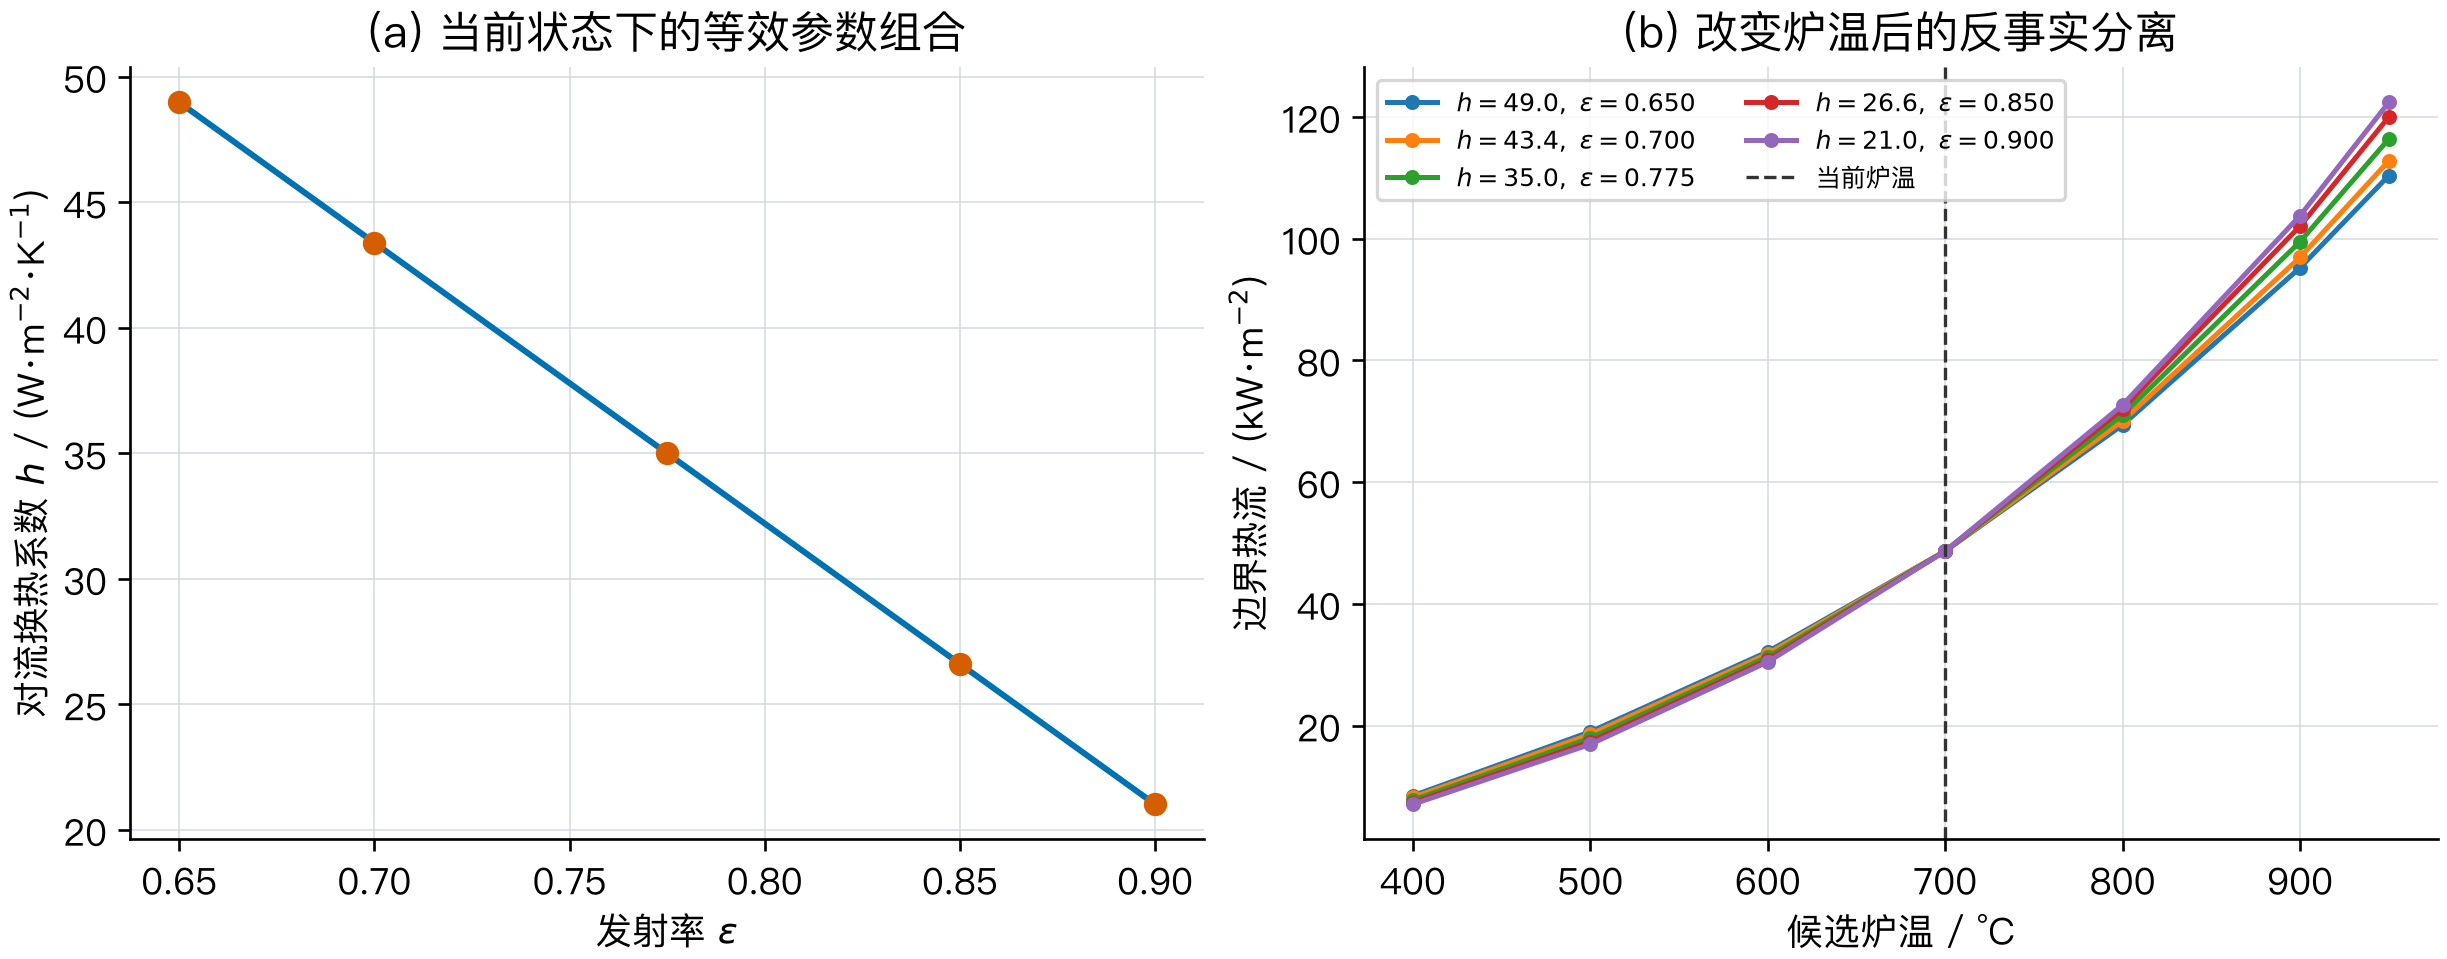
\includegraphics[width=0.98\textwidth]{counterfactual_identifiability.png}
  \caption{当前动作下的等效边界参数与候选炉温改变后的反事实热流}
  \label{fig:counterfactual_identifiability}
\end{figure}

一维等效边界世界模型写为
\begin{equation}
  \widehat{\bm{s}}_{n+1}
  =F_{\theta}^{H}(\bm{s}_n,a_n,\Heff_n,s_k,s_c,L,\Delta t).
  \label{eq:heff_model}
\end{equation}
等效边界表示将当前热流相同的参数组合归为同一输入，降低输入维数。式\eqref{eq:heff_model}省略固定密度，连续参考轨迹上的误差由留出测试评价。

训练和验证中的 $\Heff$ 由参考表面温度构造，接收该序列的完整测试推演属于参考温度条件预测。自主推演给两类模型相同的初态、动作、材料参数与真实动态 $h,\varepsilon$，等效边界模型仅从自身预测表面温度逐步重算 $\Heff$。该比较限于已知外生边界的输入表示，不能直接推定依赖因果观测与状态估计的未知边界应用。

闭环规划通过增广状态滤波器维持受历史测量约束的 $h$ 与 $\varepsilon$ 后验集合，各成员给出候选动作下的 $\Heff(a')$，保留不同参数分解在动作改变后的响应差异。

\section{评价指标与统计单位}
\label{sec:evaluation-protocol}

设测试集包含 $M$ 条轨迹，每条有 $\tau$ 次转移和 $N$ 个温度节点，完整轨迹滚动 RMSE 定义为
\begin{equation}
  \mathrm{RMSE}_{\mathrm{roll}}
  =\sqrt{\frac{1}{MN\tau}\sum_{m=1}^{M}\sum_{n=1}^{\tau}
  \left\|\widehat{\bm{s}}_{m,n}-\bm{s}_{m,n}\right\|_2^2}.
\end{equation}
该指标为全部轨迹、时刻和节点均方误差的平方根。逐轨迹 RMSE 中位数及 95\% 分位数、最大绝对误差、终态 RMSE 和离散物理残差分别描述典型轨迹、尾部、终点误差及方程一致性。最大值原理以当前全场温度与炉温的上下界为全局包络；下一状态越界则记一次违反。该指标允许邻域导热导致的合法升温或降温。

训练重复使用种子 42、7、123。表中“均值$\pm$标准差”默认表示三个训练种子的均值与样本标准差，用于描述训练重复间的变化。每次训练只用验证集选模。一维 BDF 交叉求解器参考及控制环境不用于神经模型训练；三维 BDF 轨迹则按第\ref{sec:dataset-design}节的原则划分后，分别承担训练、验证与测试用途。

方法比较以相同物理工况配对。预测实验的配对差由同一轨迹上两种方法各自的三种子指标均值之差得到，闭环实验按同一 BDF 场景执行相同处理。以轨迹或场景为重采样单位，进行 100000 次配对 bootstrap，报告平均配对差及 95\% 区间。重采样保留同一工况下方法间的对应关系，不把模型种子或轨迹中的时间点计为额外独立工况。逐轨迹 RMSE 的平均配对差与总体滚动 RMSE 的均值之差是不同统计量。

控制成功情况同时报告回合记录与场景判据。对于使用三个训练种子的学习控制器，一个回合对应一个模型在一个场景中的控制过程，场景级成功要求固定的三个模型在该场景均满足成功条件。95\% Wilson 区间以这一场景级二元结果计算，反映固定模型面板在场景抽样下的不确定性。它不等于将三个模型的回合汇总后得到的平均成功率，也不表示任意重训练模型或真实工业炉次的成功保证。温度误差、区间覆盖和控制成功分别评价，单项指标的改善不足以证明闭环整体可靠性。

\chapter{温度场预测、边界表示与计算效率}

本章评价给定炉温序列下的300步温度场预测，考察递归展开、物理损失和边界表示对误差累积的影响。测试覆盖控制曲线、材料参数及边界时间结构的外推，采用相同测试信息下的边界表示对照和跨求解器数值参考，并报告单轨迹计算代价与固定几何三维结果。炉温序列由实验设定，评价范围为开环状态递推。

\section{完整轨迹预测的模型选择}

一维 C45 温变物性数据集包含120条轨迹，其中训练、验证、ID测试和控制曲线OOD分别为70、15、15和20条。各组比较共享相同轨迹划分；归一化量由训练集确定，检查点依据验证集300步滚动RMSE选择。除单种子计时外，结果均报告种子42、7和123的均值与样本标准差。种子间标准差描述训练随机性，场景差异采用独立轨迹配对统计。

\subsection{递归展开与误差累积}

递归推演的输入温度场来自模型上一时刻的预测。展开长度比较设置 $K=1$ 与 $K=5$，两组共享70条训练轨迹、网络容量、物理权重 $10^{-3}$、批量大小、120轮训练和三个随机种子。表\ref{tab:unroll_ablation}同时列出一步误差与完整轨迹误差。

\begin{table}[H]
  \centering
  \caption{相同训练设置下的展开长度消融，均值$\pm$样本标准差}
  \label{tab:unroll_ablation}
  \small
  \begin{tabular}{ccccc}
    \toprule
    $K$ & \shortstack{验证滚动\\RMSE} & \shortstack{ID 滚动\\RMSE} & \shortstack{控制 OOD\\滚动 RMSE} & \shortstack{ID 一步\\RMSE} \\
    \midrule
    1 & $2.063\pm0.187$ & $2.196\pm0.005$ & $\mathbf{5.046\pm0.469}$ & $0.02862\pm0.00029$ \\
    5 & $\mathbf{2.035\pm0.244}$ & $\mathbf{2.103\pm0.123}$ & $5.589\pm0.789$ & $0.02848\pm0.00184$ \\
    \bottomrule
  \end{tabular}
\end{table}

两种设置的ID一步RMSE均约为 \SI{0.0285}{\degreeCelsius}，完整轨迹RMSE约为 \SI{2}{\degreeCelsius}，递归误差明显累积。$K=5$ 的验证和ID滚动RMSE均值分别比 $K=1$ 低 $1.3\%$ 和 $4.2\%$，控制OOD均值高 $10.8\%$。依据验证均值，本文选择 $K=5$；其收益限于当前验证和ID结果，控制曲线外推误差随展开长度增加而增大。

\subsection{物理约束强度与控制曲线外推}

在 $K=5$ 下，数据模型与物理约束模型仅改变损失中的物理权重，比较结果见表\ref{tab:weight_results}。控制OOD采用未见炉温曲线类型，评价留出控制过程中的响应误差；检查点仍由验证集选择。

\begin{table}[H]
  \centering
  \caption{不同物理权重的三随机种子结果，均值$\pm$样本标准差}
  \label{tab:weight_results}
  \small
  \begin{tabular}{ccccc}
    \toprule
    $\lambda_{\mathrm{phy}}$ & 验证 RMSE & ID RMSE & OOD RMSE & OOD 物理残差 \\
    \midrule
    0 & $2.282\pm0.109$ & $2.389\pm0.139$ & $5.994\pm0.430$ & $127.41\pm7.36$ \\
    $10^{-3}$ & $\mathbf{2.035\pm0.244}$ & $\mathbf{2.103\pm0.123}$ & $\mathbf{5.589\pm0.789}$ & $70.35\pm4.24$ \\
    $10^{-2}$ & $2.242\pm0.109$ & $2.739\pm0.107$ & $6.865\pm1.202$ & $\mathbf{60.29\pm10.42}$ \\
    \bottomrule
  \end{tabular}
\end{table}

$\lambda_{\mathrm{phy}}=10^{-3}$ 的验证RMSE均值最低，选为一维模型的正式权重。相对数据模型，其ID误差均值降低 $11.9\%$，控制OOD总体RMSE均值降低 $6.8\%$，OOD离散物理残差降低 $44.8\%$；其中升温后冷却轨迹的RMSE均值降低 $10.1\%$。权重增至 $10^{-2}$ 后，离散残差减小，温度场误差增加。两项指标随权重呈不同变化，模型选择以验证轨迹精度为依据。

配对统计采用每条控制OOD轨迹三个种子RMSE的平均值，差值定义为物理模型减去数据模型。20条轨迹中12条改善、8条变差，平均配对差为 \SI{-0.220}{\degreeCelsius}；以轨迹为单位进行100000次bootstrap，95\%区间为 $[-0.588,0.153]$~\si{\degreeCelsius}。区间包含零，$6.8\%$ 的总体均值降幅仅构成当前样本中的改善趋势，稳定的控制OOD精度收益缺乏统计支持。各物理权重的重复结果见图\ref{fig:weight_results}。

\begin{figure}[H]
  \centering
  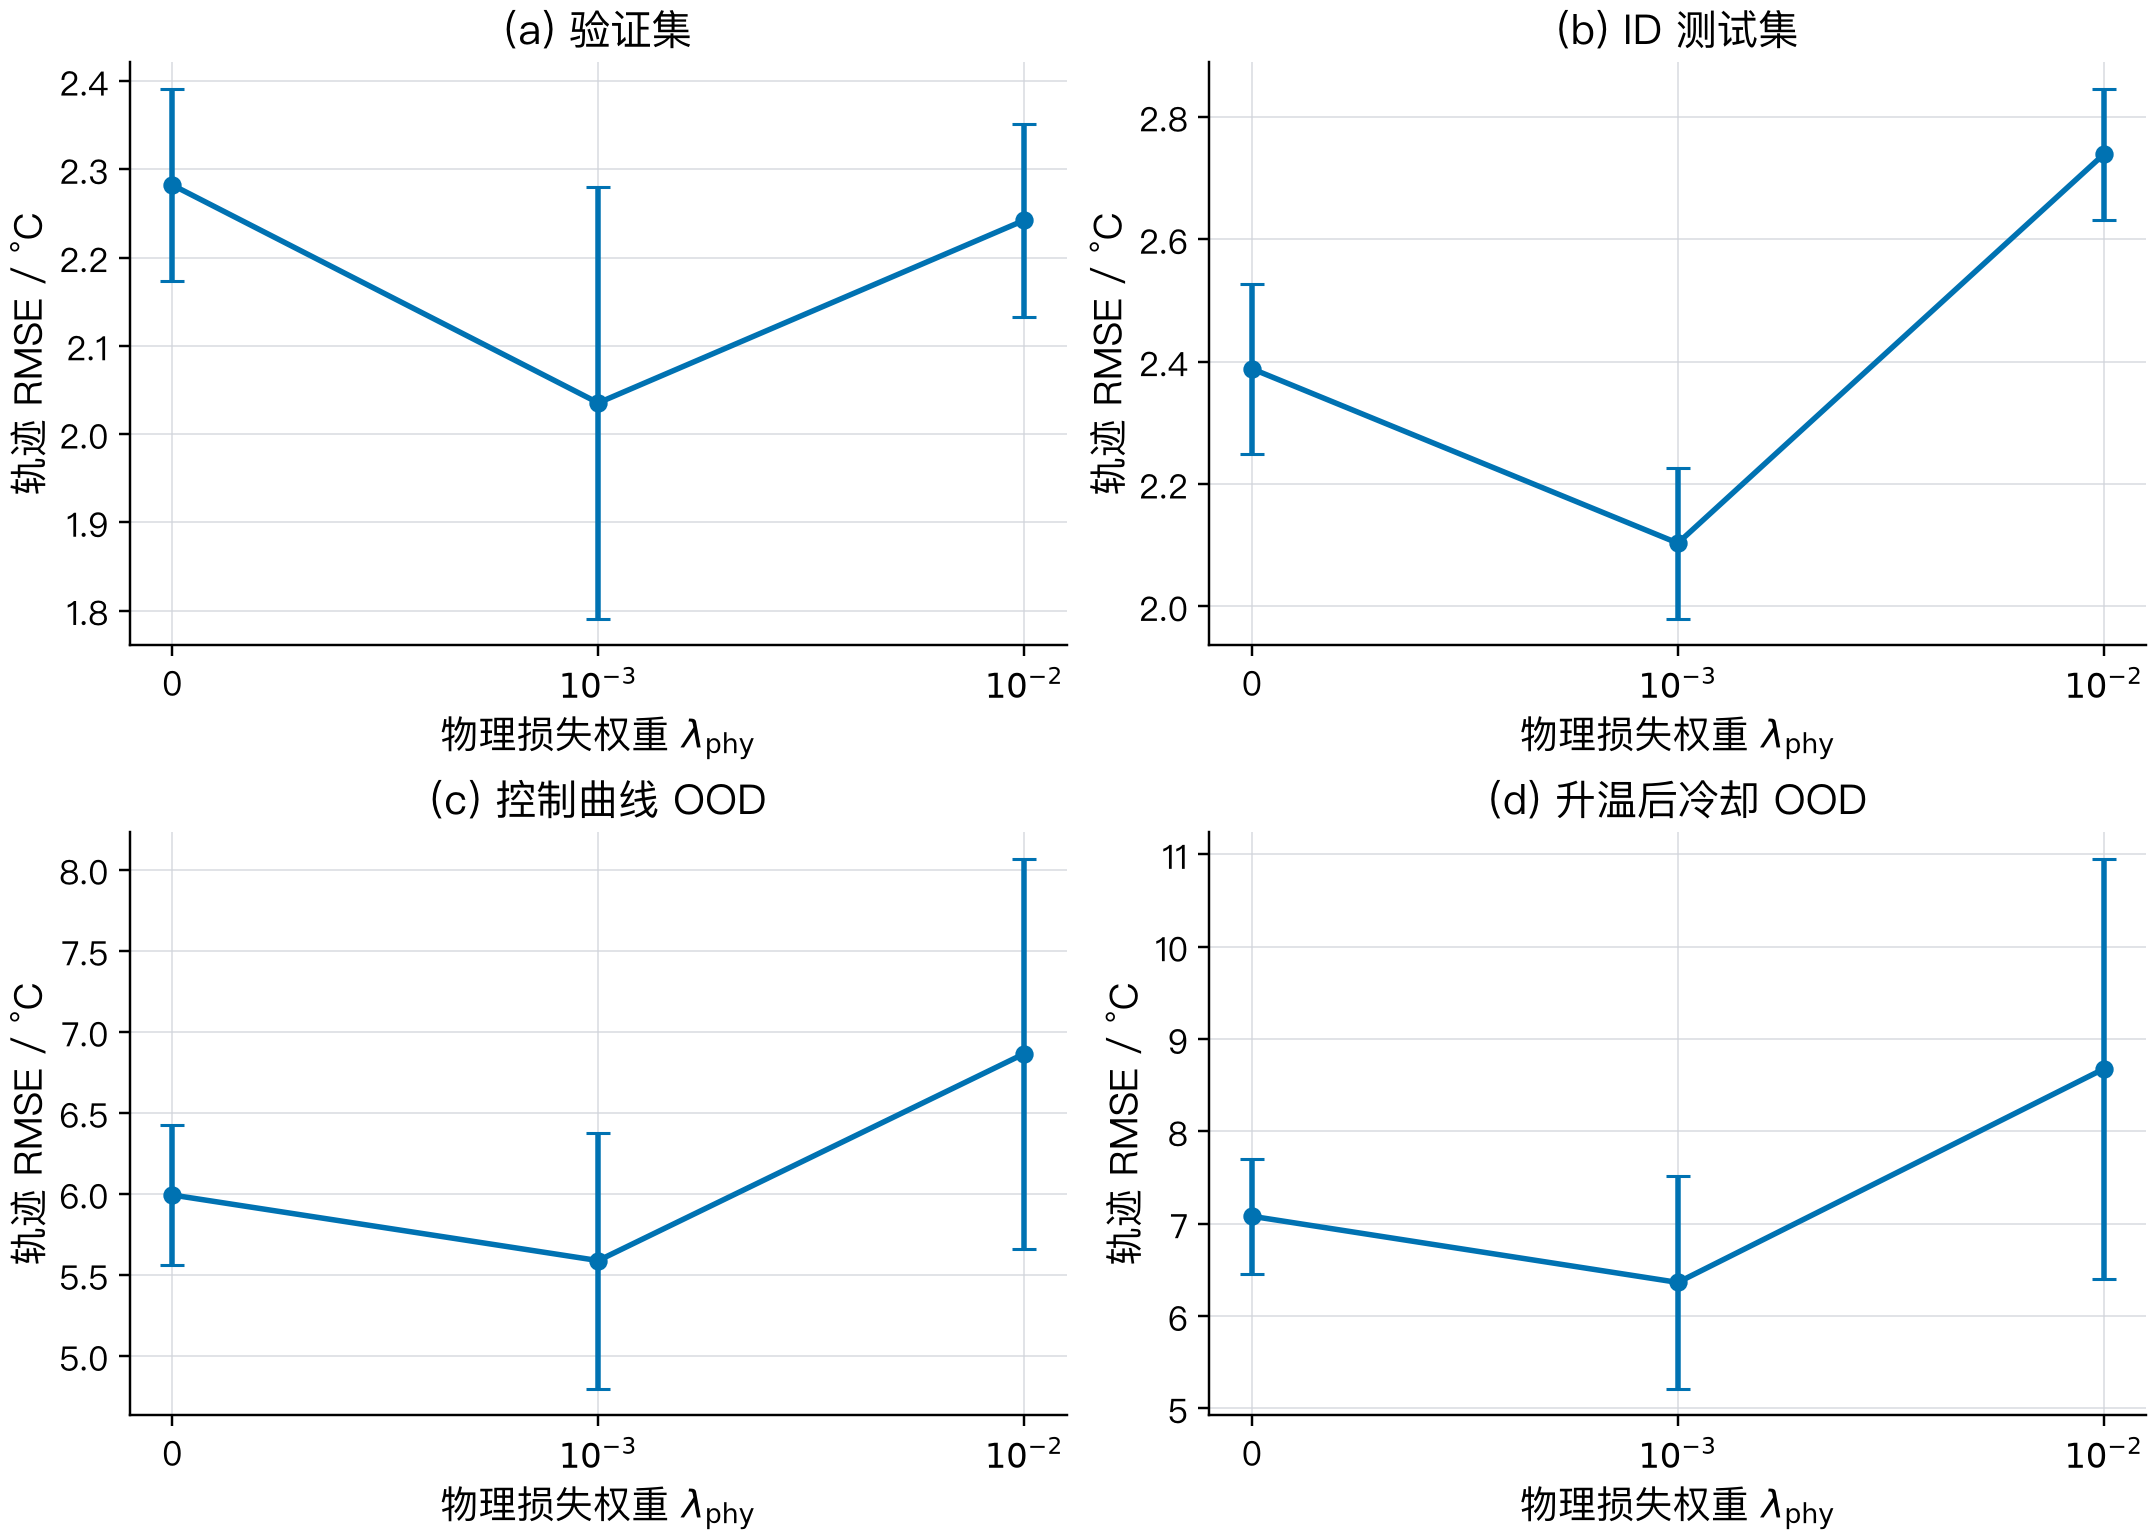
\includegraphics[width=0.96\textwidth]{physics_weight_replicates.png}
  \caption{物理权重在 ID 与控制 OOD 条件下的重复实验结果}
  \label{fig:weight_results}
\end{figure}

\section{参数外推与边界时间结构}

\subsection{材料及边界参数范围的外推}

参数OOD集的控制曲线保持为训练类型，对流换热系数、发射率、导热系数尺度和比热尺度各设置20条单因素轨迹，另设置20条四参数组合轨迹，共100条。表\ref{tab:param_ood}比较数据模型与正式物理权重下的三种子结果。

\begin{table}[H]
  \centering
  \caption{参数 OOD 的滚动 RMSE，单位：\si{\degreeCelsius}}
  \label{tab:param_ood}
  \begin{tabular}{lccc}
    \toprule
    OOD 类型 & 数据模型 & 物理模型 & 相对降低 \\
    \midrule
    对流换热系数 $h$ & $3.082\pm0.259$ & $2.693\pm0.613$ & $12.6\%$ \\
    发射率 $\varepsilon$ & $3.239\pm0.290$ & $3.046\pm0.507$ & $6.0\%$ \\
    导热系数尺度 $s_k$ & $7.369\pm0.702$ & $5.633\pm0.397$ & $23.6\%$ \\
    比热尺度 $s_c$ & $5.802\pm0.445$ & $5.672\pm0.953$ & $2.2\%$ \\
    四参数组合 & $16.991\pm2.893$ & $11.972\pm2.534$ & $29.5\%$ \\
    \bottomrule
  \end{tabular}
\end{table}

五类参数OOD的平均RMSE均有所降低，其中导热系数尺度和四参数组合在三个种子下都得到改善。四参数组合的滚动RMSE由 $16.991\pm2.893$ 降至 $11.972\pm2.534$~\si{\degreeCelsius}，降幅为 $29.5\%$；最大绝对误差由 $121.76\pm30.94$ 降至 $61.69\pm16.41$~\si{\degreeCelsius}，离散物理残差由 $614.78\pm45.47$ 降至 $233.62\pm27.30$~\si{\degreeCelsius}。多参数偏移同时改变热扩散时间尺度和表面热流，组合工况在本组参数测试中的平均误差降幅最大。这些误差降幅仅适用于所测试的参数分布。

\begin{figure}[H]
  \centering
  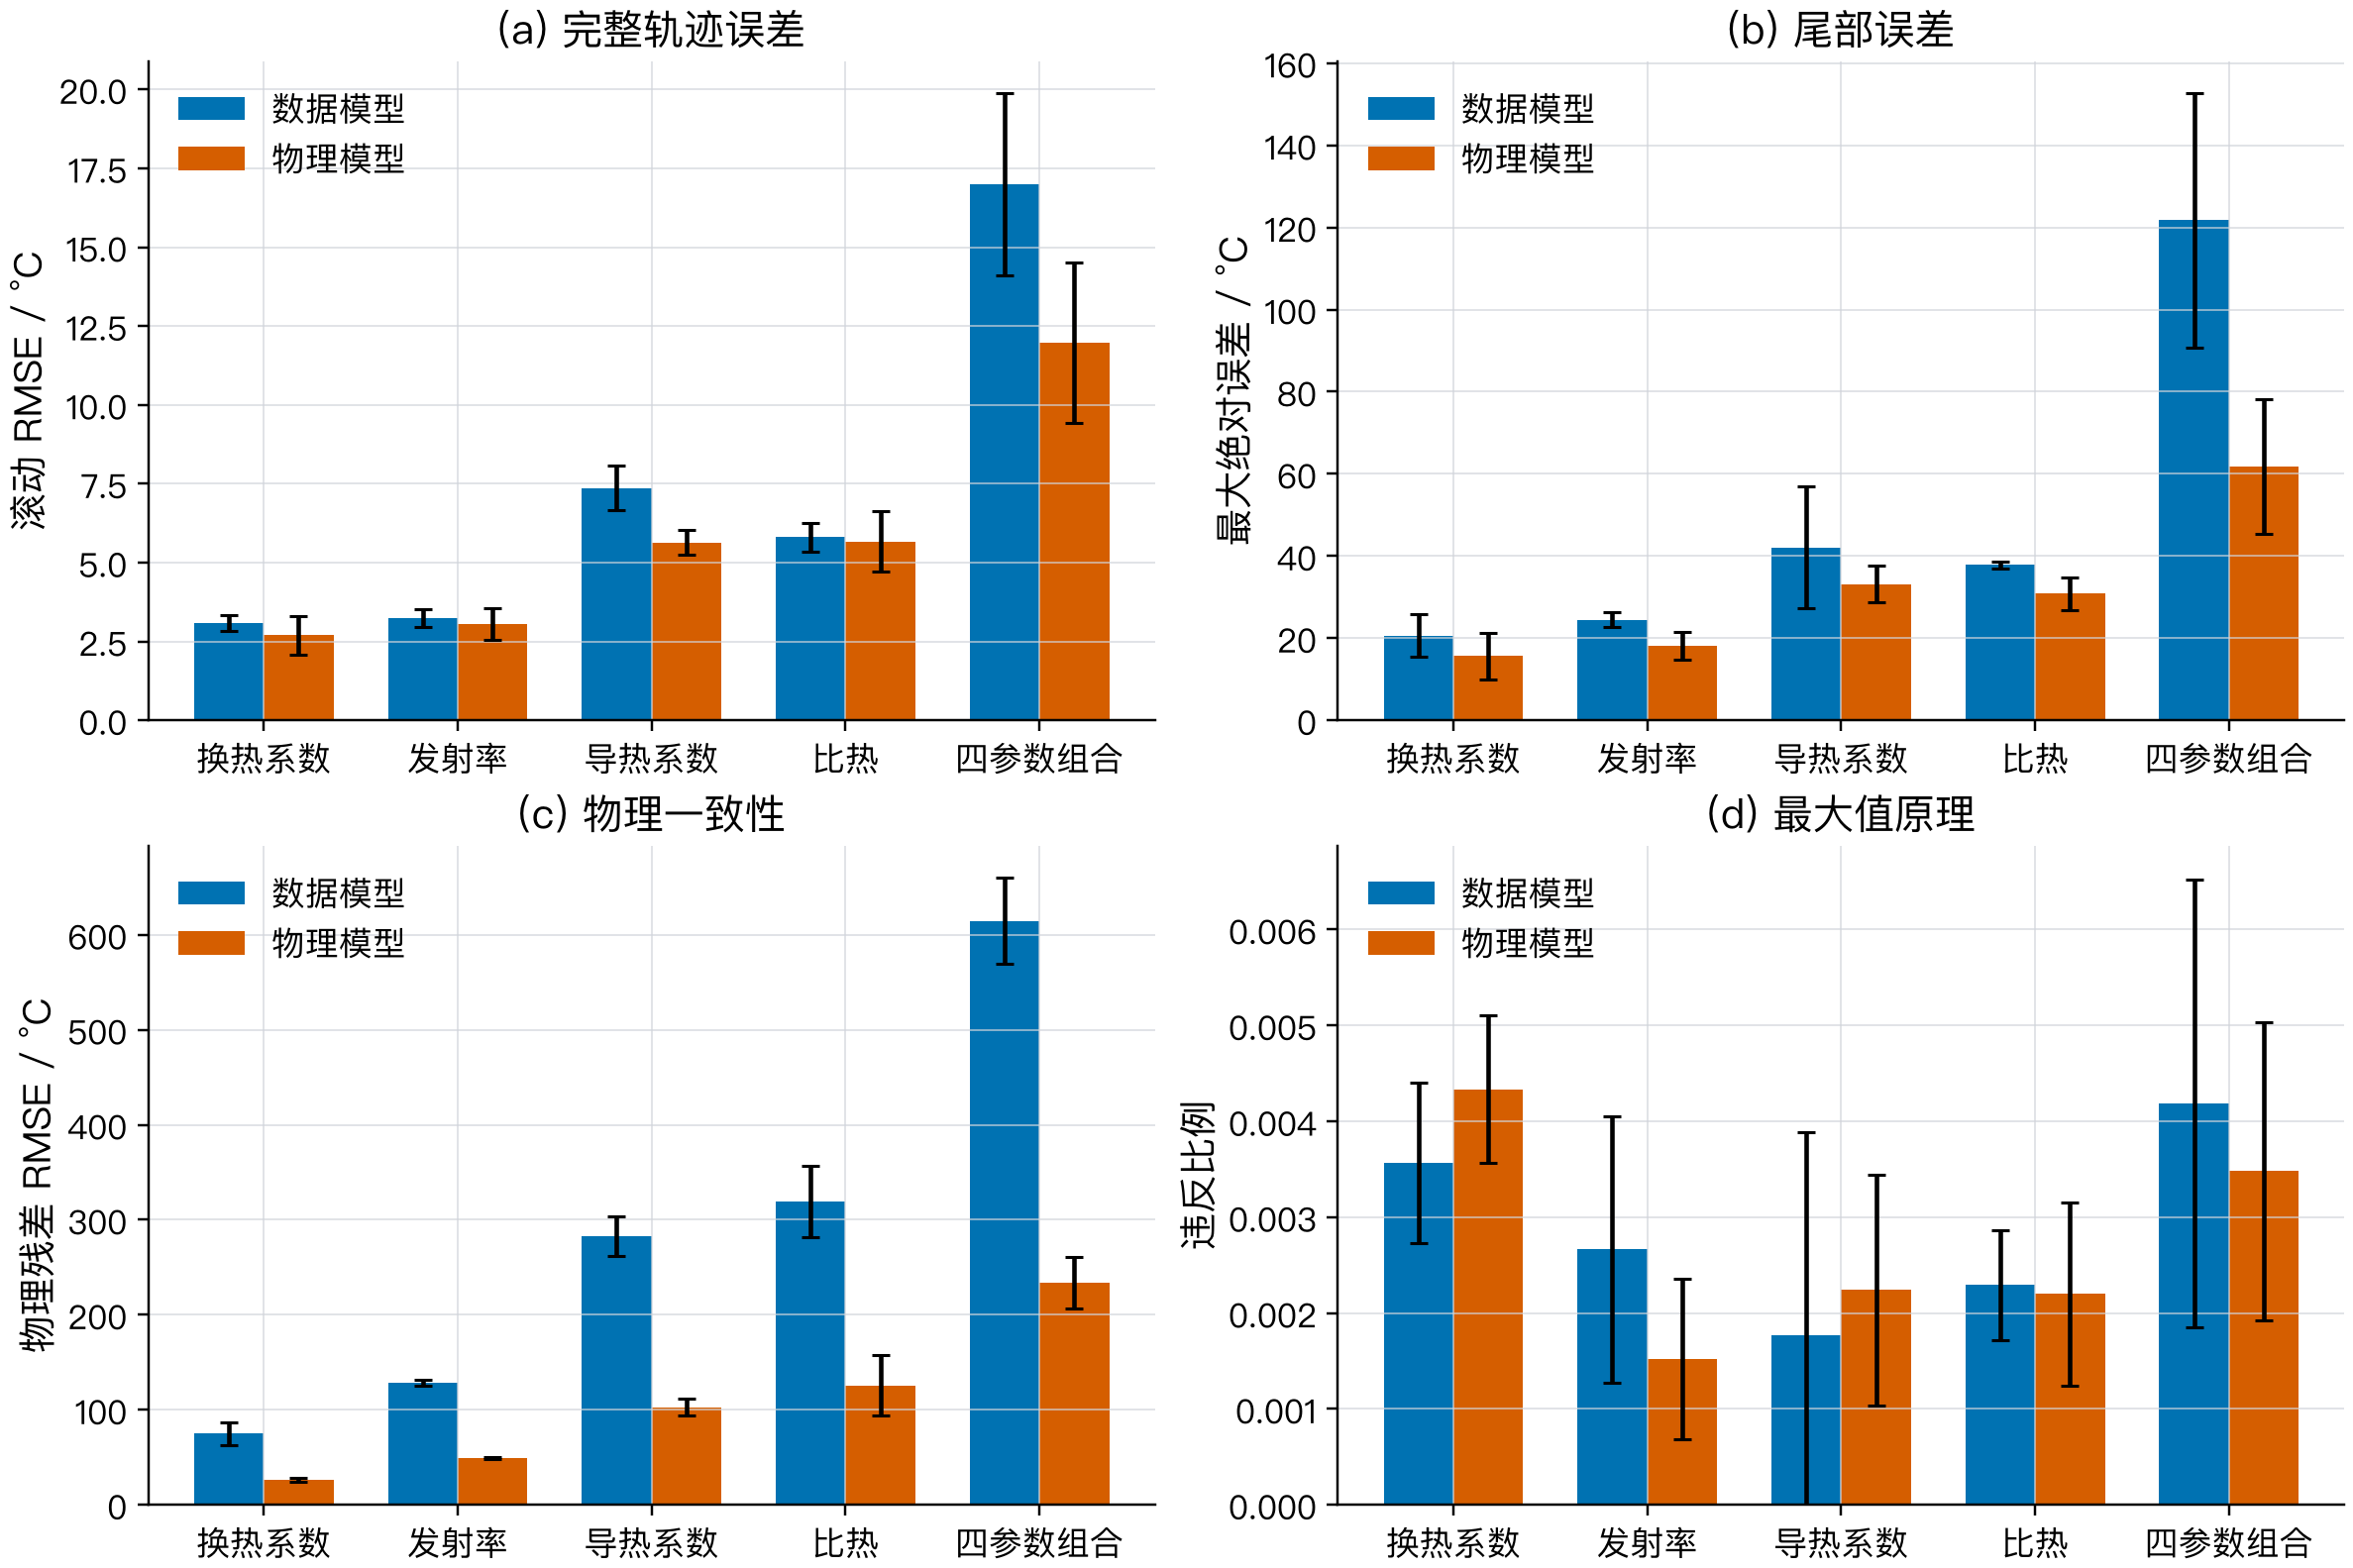
\includegraphics[width=0.96\textwidth]{parameter_ood_metrics.png}
  \caption{不同参数 OOD 类别的温度场推演误差}
  \label{fig:param_ood}
\end{figure}

\subsection{时变边界与逐步输入}

动态边界实验将参数值限制在训练范围内，只改变其时间结构。测试包含 $h$ 平滑变化、$h$ 阶跃、$\varepsilon$ 增长、$\varepsilon$ 阶跃和联合变化五类，共100条轨迹；训练轨迹中的边界参数在单条轨迹内保持常数。该设计评价训练参数范围内的时间结构外推。

逐步提供真实 $h(t)$ 和 $\varepsilon(t)$ 时，数据模型滚动RMSE为 $4.795\pm0.289$~\si{\degreeCelsius}，物理模型为 $4.089\pm0.162$~\si{\degreeCelsius}，均值降低 $14.7\%$；物理残差降低 $57.3\%$，逐轨迹RMSE的95\%分位数降低 $13.0\%$。整段推演固定使用首时刻参数时，两类模型的RMSE均约为 \SI{19.4}{\degreeCelsius}。固定边界引起的误差增幅大于两种损失设置之间的差异，两类模型均依赖逐步更新的边界信息。

图\ref{fig:dynamic_trajectory}取联合边界变化类别中的中位误差轨迹。在300~s内对流与辐射条件连续变化，模型接收逐步更新的真实边界值；物理模型在中心和表面位置均跟踪数值参考。该例评价真实时变边界已知条件下的预测，边界表示对照与未知边界估计分别在后续实验中处理。

\begin{figure}[H]
  \centering
  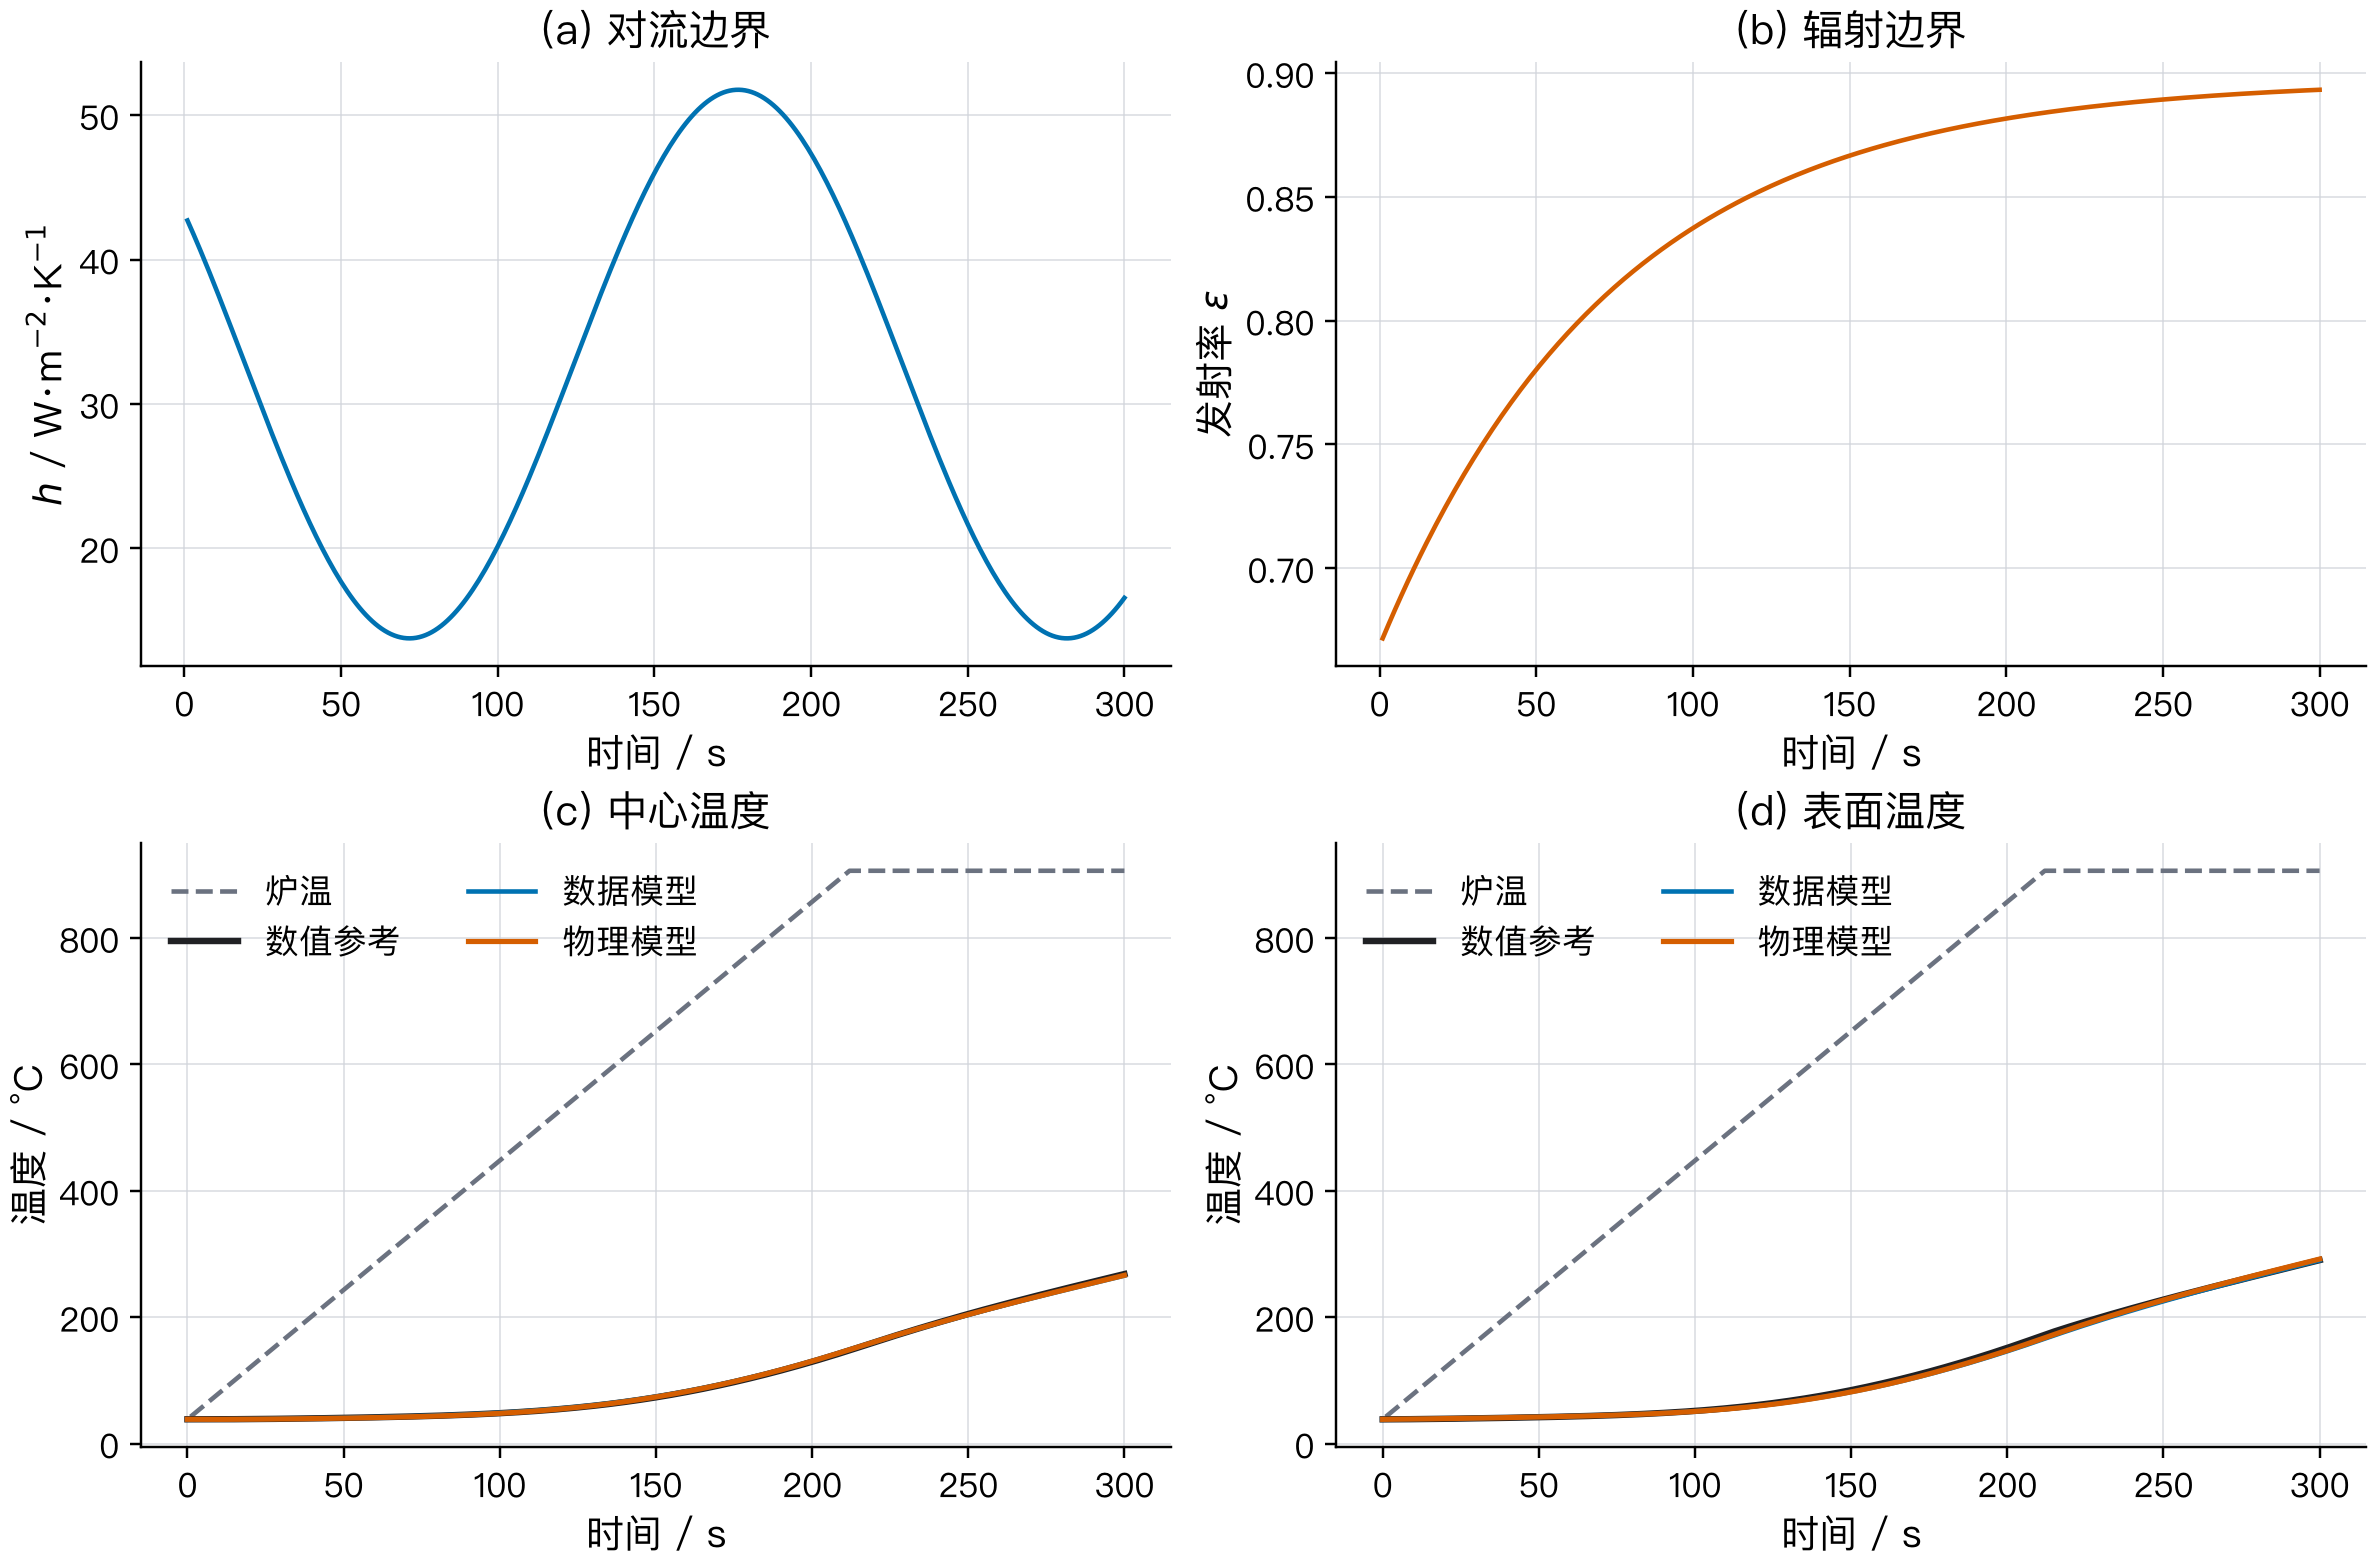
\includegraphics[width=0.96\textwidth]{dynamic_boundary_trajectory_zh.png}
  \caption{联合动态边界下的代表性温度场推演轨迹}
  \label{fig:dynamic_trajectory}
\end{figure}

\section{等效边界表示与测试信息条件}

式\eqref{eq:heff}将当前对流与辐射热流写为等效换热系数 $\Heff$ 与边界温差的乘积。边界表示实验分别评价预测状态重算和参考状态条件输入。参考状态条件输入包含额外的表面温度信息，与直接接收 $h,\varepsilon$ 的自主模型具有不同的测试信息条件。

等效边界模型使用同一组120条静态边界轨迹，将每个转移的输入转换为 $\Heff$，保持训练、验证与测试划分、网络宽度和深度、训练轮数、随机种子及物理损失权重一致。多步训练和验证检查点选择采用由参考状态构造的 $\Heff$ 序列：温度场按网络输出递归，系数始终取自参考状态。自主滚动评价固定这些模型权重和检查点，未利用测试结果重新训练或选模。“自主”限定于测试推理阶段的系数更新，训练与验证仍采用参考状态条件输入。

测试使用另一组动态边界留出轨迹，同样包含五类边界变化、每类20条，共100条，每条递推300步。它与上一节动态边界测试属于不同抽样，误差不作跨数据集的直接差值比较。两种自主模型均获得相同的初始温度场、炉温序列、真实动态 $h,\varepsilon$ 和材料几何参数。原始参数模型直接使用 $h,\varepsilon$；等效边界模型在每一步取自身两端预测表面温度的平均值，代入式\eqref{eq:heff}重算 $\Heff$，不读取后续参考温度。参考表面温度条件输入作为单独的诊断对照列出。表\ref{tab:heff_results}中的模型物理权重均为 $10^{-3}$，离散残差统一使用真实 $h,\varepsilon$ 和各自预测状态计算。

\begin{table}[H]
  \centering
  \caption{动态边界留出集上的边界表示比较：三种子均值$\pm$样本标准差}
  \label{tab:heff_results}
  \begin{tabular}{lcc}
    \toprule
    边界输入与测试方式 & 滚动 RMSE/\si{\degreeCelsius} & 物理残差/\si{\degreeCelsius} \\
    \midrule
    $h,\varepsilon$，真实动态值 & $2.285\pm0.108$ & $17.79\pm1.59$ \\
    $\Heff$，由预测表面温度重算 & $1.494\pm0.082$ & $17.37\pm2.79$ \\
    $\Heff$，参考表面温度条件输入 & $1.409\pm0.068$ & $17.38\pm2.81$ \\
    \bottomrule
  \end{tabular}
\end{table}

相同测试信息下，滚动RMSE由 $2.285\pm0.108$ 降至 $1.494\pm0.082$~\si{\degreeCelsius}，均值降低 $34.6\%$。配对统计使用各轨迹三个种子RMSE的平均值，对100条轨迹进行100000次bootstrap，等效边界模型减去原始参数模型的配对差均值为 \SI{-0.459}{\degreeCelsius}，95\%区间为 $[-0.638,-0.305]$~\si{\degreeCelsius}，82/100条轨迹改善。该配对差基于逐轨迹RMSE的均值，与表中全场总体RMSE均值之差具有不同的汇总次序。

参考状态条件输入的误差为 $1.409\pm0.068$~\si{\degreeCelsius}，相对原始参数模型降低 $38.3\%$，其中包含额外状态信息的影响。自主预测对应的同信息降幅为 $34.6\%$。这组比较支持已知动态参数序列下、采用参考状态系数训练和验证的等效边界模型；完全自主系数训练与未知边界辨识均未在该对照中检验。未知边界的因果观测与状态估计见下一章。

\section{跨求解器验证与计算代价}

\subsection{改变参考离散后的预测误差}

一维模型的训练数据与物理损失采用同一固定时间步长离散系统。跨求解器测试对边界表示留出集的相同100条物理工况，采用81节点空间离散和 SciPy 自适应BDF时间积分求解，并将参考场投影到模型网格。BDF轨迹仅用于评价，不参与网络训练与检查点选择。表\ref{tab:cross_solver}同时列出两种边界表示的数据模型与物理模型结果。

\begin{table}[H]
  \centering
  \caption{BDF 参考轨迹上的跨求解器数值验证}
  \label{tab:cross_solver}
  \begin{tabular}{lcc}
    \toprule
    模型 & 滚动 RMSE/\si{\degreeCelsius} & 最大绝对误差/\si{\degreeCelsius} \\
    \midrule
    $h,\varepsilon$ 数据模型 & $2.539\pm0.018$ & $25.56\pm0.43$ \\
    $h,\varepsilon$ 物理模型 & $2.316\pm0.092$ & $21.87\pm2.71$ \\
    $\Heff$ 数据模型，自主重算 & $1.551\pm0.050$ & $14.33\pm4.46$ \\
    $\Heff$ 物理模型，自主重算 & $1.560\pm0.092$ & $11.78\pm0.74$ \\
    $\Heff$ 数据模型，参考状态条件输入 & $1.491\pm0.065$ & $14.27\pm4.05$ \\
    $\Heff$ 物理模型，参考状态条件输入 & $1.460\pm0.078$ & $9.75\pm0.20$ \\
    \bottomrule
  \end{tabular}
\end{table}

在相同测试信息下，自主 $\Heff$ 物理模型相对 $h,\varepsilon$ 物理模型的总体RMSE均值降低 $32.6\%$，最大绝对误差均值降低 $46.1\%$。采用与前节相同的轨迹配对和100000次bootstrap方法，RMSE配对差均值为 \SI{-0.415}{\degreeCelsius}，95\%区间为 $[-0.598,-0.260]$~\si{\degreeCelsius}，80/100条轨迹改善。图\ref{fig:cross_solver_summary}将两套数值参考上的结果并列，等效边界模型的预测改善在BDF参考上仍然存在。

同一种自主 $\Heff$ 表示下，物理模型的总体RMSE为 \SI{1.560}{\degreeCelsius}，高于数据模型的 \SI{1.551}{\degreeCelsius}，最大绝对误差则较低。参考状态条件结果包含额外温度信息；所有 $\Heff$ 模型的训练与验证条件均保持前节设置。两套参考共用100条物理工况，按200个独立场景合并统计会重复计数。跨求解器结果评价数值实现变化下的预测表现，真实炉体验证仍待开展。

\begin{figure}[H]
  \centering
  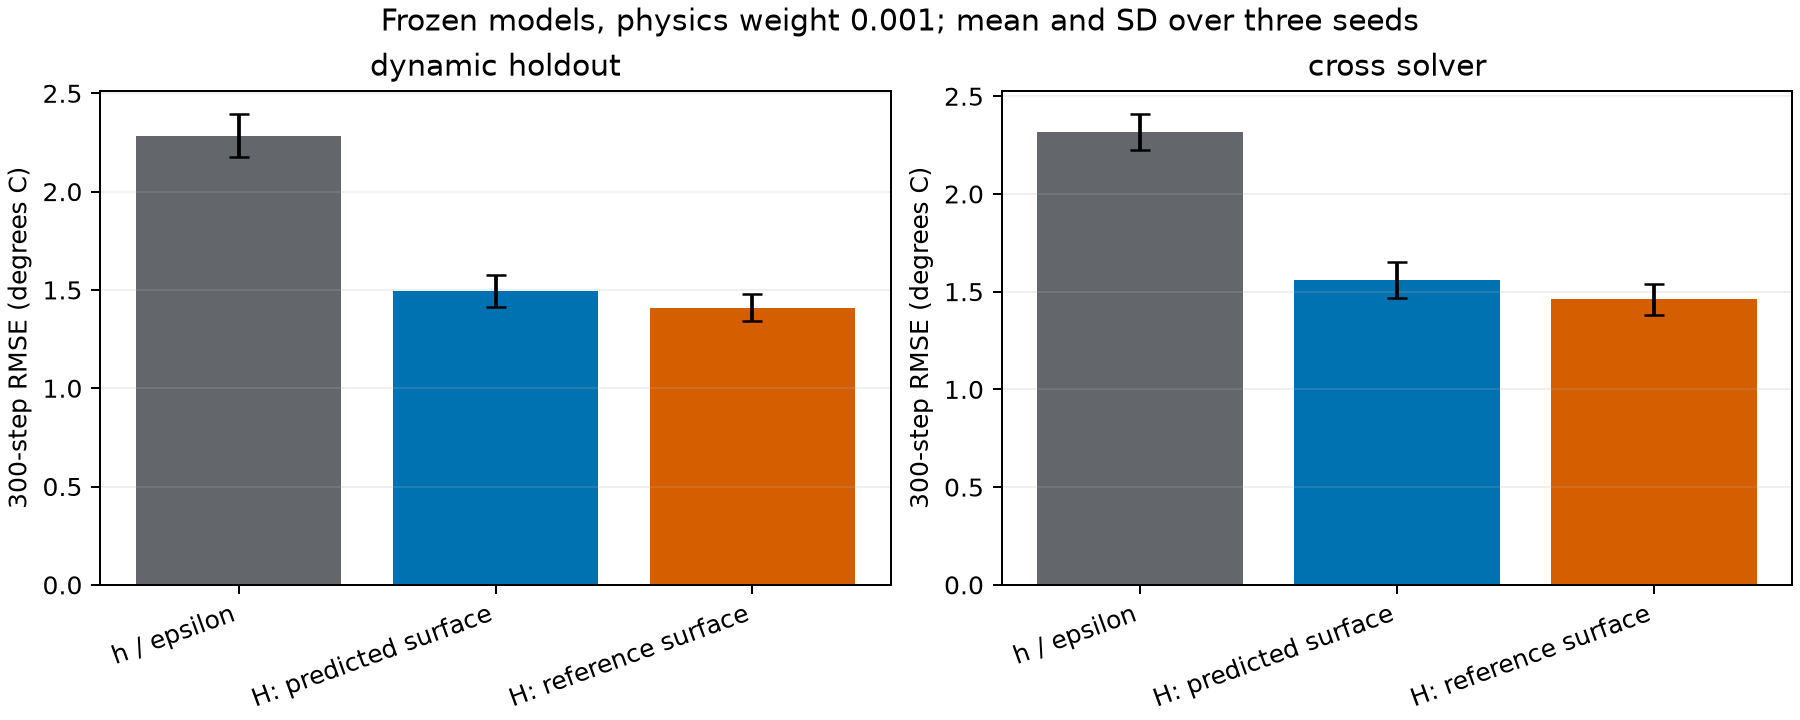
\includegraphics[width=0.98\textwidth]{fair_boundary_comparison.png}
  \caption{同信息自主滚动与参考表面温度条件输入的比较，误差棒表示三个训练种子的样本标准差}
  \label{fig:cross_solver_summary}
\end{figure}

图\ref{fig:cross_solver_trajectory}采用联合边界类别中、两种数值求解器差异最接近类别中位数的轨迹。固定步长数值解与BDF解在该例中接近。图内 $\Heff$ 曲线使用参考状态构造系数，展示条件输入下的时间响应；自主重算精度由表\ref{tab:cross_solver}单独报告。

\begin{figure}[H]
  \centering
  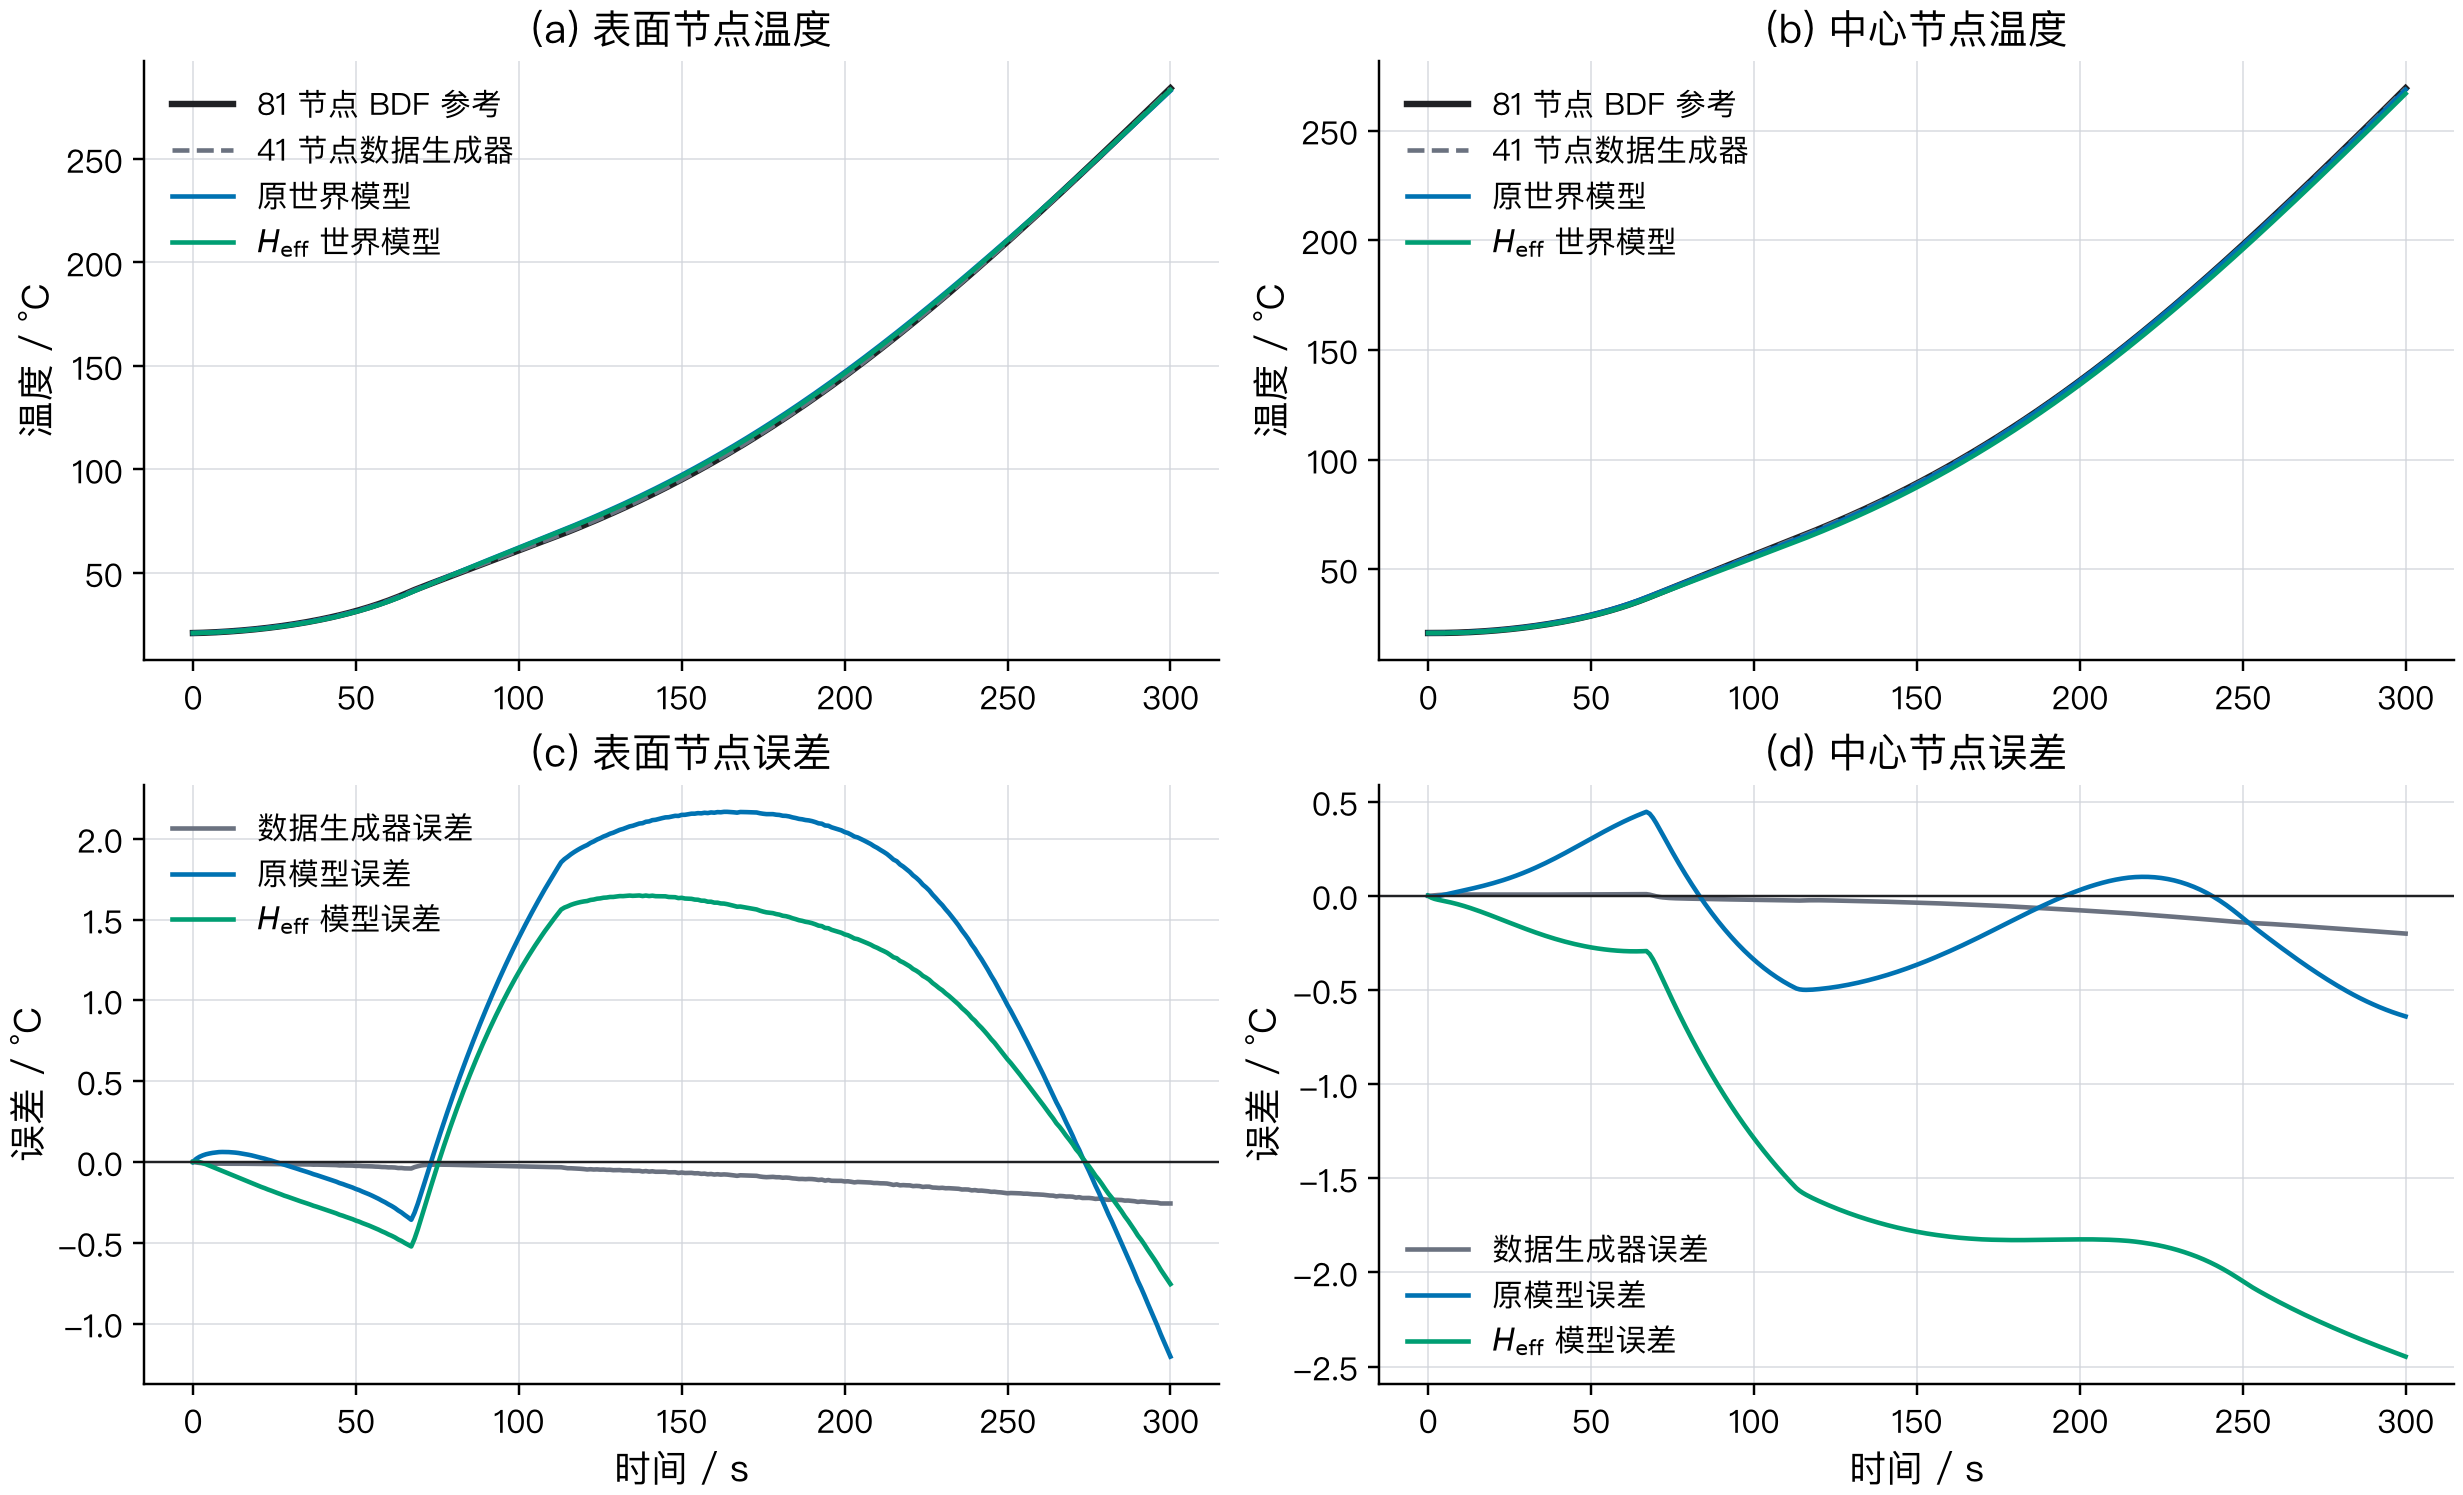
\includegraphics[width=0.96\textwidth]{cross_solver_trajectory_zh.png}
  \caption{代表性动态边界轨迹的跨求解器温度曲线（有效边界采用参考状态条件输入）}
  \label{fig:cross_solver_trajectory}
\end{figure}

\subsection{相同工作量下的单轨迹计算代价}

计时比较在 Apple M5 CPU 上以单线程运行，使用上述相同100条输入轨迹，每条包含300步转移。神经模型固定为种子42、物理权重0.001，比较原始 $h,\varepsilon$ 网络、自主 $\Heff$ 网络、41节点固定步长数值模型和81节点BDF。BDF相对与绝对容差分别为 $10^{-6}$ 和 $10^{-7}$，最大步长为 \SI{0.25}{\second}。

四种方法均预热一整轮，正式计时三整轮，每条场景内随机排列方法顺序；每种方法的300次计时来自100条不同工况。计时包含输入转换、自主 $\Heff$ 更新、输出数组形成及BDF投影，模型载入与求解器构造均不计入，运行期间暂停其他实验计算。表\ref{tab:fair_timing}同时给出耗时和相对缓存BDF参考解的误差，精度指标对应单个种子，与三种子结果分别报告。

\begin{table}[H]
  \centering
  \caption{相同 100 条场景完整推演的耗时与精度（每种方法 300 次计时）}
  \label{tab:fair_timing}
  \begin{tabular}{lrrr}
    \toprule
    方法 & 中位耗时/ms & 95 分位/ms & RMSE/\si{\degreeCelsius} \\
    \midrule
    原始 $h,\varepsilon$ 网络 & 8.116 & 8.607 & 2.345 \\
    自主 $\Heff$ 网络 & 10.284 & 10.962 & 1.474 \\
    41 节点固定步长数值模型 & 10.873 & 11.351 & 0.166 \\
    81 节点 BDF & 452.847 & 562.346 & $4.1\times10^{-6}$ \\
    \bottomrule
  \end{tabular}
\end{table}

81节点BDF的中位耗时是自主 $\Heff$ 网络的44.0倍；41节点固定步长数值模型的中位耗时为该网络的1.06倍，RMSE更低。比较固定了实现和离散配置，未匹配数值方法与网络的预测精度。网络相对于BDF复核器具有计算余量，相对于简单数值模型的一维单轨迹精度与效率综合优势尚未确立。

下一章的63.4倍规划耗时比对应完整状态及未来边界已知条件下的候选动作搜索，本节的44.0倍对应一次完整轨迹预测，两者的工作量与信息条件不同。候选动作批量推演的同精度数值基准、优化降阶模型对照及三维闭环计时仍未完成，速度结论限于所报告的任务和基准。

\section{三维温度场的递推与误差结构}

\subsection{固定几何下的训练与评价协议}

三维实验评价固定几何下较多温度状态的受控递推。三维热模型可用于表达氧化层、支承遮蔽和各表面非均匀受热的影响\cite{yang2022reheating3d}；本节采用均匀六面边界，不包含这些复杂表面条件。C45试块尺寸为 \SI{60}{\milli\metre}$\times$\SI{40}{\milli\metre}$\times$\SI{20}{\milli\metre}，材料物性和对流--辐射边界与一维模型一致。

基础网格为 $9\times7\times5$，含315个温度状态；加密网格为 $17\times13\times9$，含1989个状态。两套网格均用方法线与BDF生成参考轨迹，每条包含300个 \SI{1}{\second} 转移。96条工况的初态、炉温指令、材料参数和划分在两网格间一致，训练、验证、ID测试和控制OOD分别为56、12、12和16条。两套网格合计192条参考轨迹，共享上述物理工况。

参考求解器、网络和离散残差采用相同的分段常值动作定义：$T_\infty(t)=a_n$，$t_n\le t<t_{n+1}$。BDF在动作改变处重新启动积分，避免跨越不连续点。网络输入包含当前温度场、炉温动作、$h$、$\varepsilon$、导热系数尺度、比热尺度以及三个空间坐标通道。卷积状态转移器含3个残差块、16个隐藏通道，共45489个参数，训练采用三步递归展开、AdamW优化器和 $8\times10^{-4}$ 的初始学习率。

种子42、7和123下的数据模型与物理模型共享工况、网络容量和初始化规则。基础网格两类模型均训练40轮，批量大小256，每5轮进行300步验证推演，并在第1轮额外验证。加密网格均训练12轮，批量大小64，每2轮验证一次，并在第1轮额外验证；每个模型分别从对应种子、对应类型的基础模型迁移16个形状相容的卷积参数张量。加密网格的坐标和归一化量重新计算，归一化及损失尺度只使用训练集。

物理损失采用六面控制体的半隐式能量平衡残差，权重预先固定为 $10^{-1}$，不与一维实验的 $10^{-3}$ 直接比较。学习率调整和检查点选择依据验证集300步滚动RMSE，测试集只在选模后评价，权重和训练预算不按测试表现调整。网格加密同时改变参考离散，并引入迁移训练阶段，因而两组学习误差的变化不能用来推断连续解的网格收敛性。

\subsection{完整轨迹误差与离散残差}

表\ref{tab:three-dimensional-zoh-base}和表\ref{tab:three-dimensional-zoh-refined}报告三种子均值与样本标准差。滚动RMSE为完整温度轨迹总体均方误差的平方根；终态平均RMSE为各轨迹末时刻空间RMSE的算术平均。离散残差评价预测与所用半隐式方程的一致性，独立温度误差另行报告，连续能量守恒尚缺少独立检验。

\begin{table}[H]
\centering
\small
\setlength{\tabcolsep}{4pt}
\caption{三维基础网格 $9\times7\times5$：三种子均值$\pm$样本标准差，单位为 $^\circ\mathrm{C}$。}
\label{tab:three-dimensional-zoh-base}
\begin{tabular}{llccc}
\toprule
划分 & 模型 & 滚动 RMSE & 终态平均 RMSE & 离散残差 RMSE \\
\midrule
验证集 & 数据模型 & $4.963\pm0.484$ & $7.566\pm1.177$ & $2.318\pm0.357$ \\
验证集 & 物理约束模型 & $4.707\pm0.541$ & $6.515\pm0.835$ & $1.776\pm0.076$ \\
ID 测试 & 数据模型 & $4.423\pm0.604$ & $6.571\pm1.414$ & $2.216\pm0.427$ \\
ID 测试 & 物理约束模型 & $4.465\pm0.556$ & $5.889\pm0.453$ & $1.758\pm0.148$ \\
控制 OOD & 数据模型 & $14.792\pm1.895$ & $23.476\pm3.790$ & $3.677\pm0.366$ \\
控制 OOD & 物理约束模型 & $16.368\pm4.713$ & $25.309\pm8.356$ & $3.218\pm0.249$ \\
\bottomrule
\end{tabular}
\end{table}

\begin{table}[H]
\centering
\small
\setlength{\tabcolsep}{4pt}
\caption{三维加密网格 $17\times13\times9$：三种子均值$\pm$样本标准差，单位为 $^\circ\mathrm{C}$。}
\label{tab:three-dimensional-zoh-refined}
\begin{tabular}{llccc}
\toprule
划分 & 模型 & 滚动 RMSE & 终态平均 RMSE & 离散残差 RMSE \\
\midrule
验证集 & 数据模型 & $4.466\pm0.349$ & $6.474\pm0.379$ & $5.042\pm0.246$ \\
验证集 & 物理约束模型 & $4.012\pm0.473$ & $5.586\pm0.660$ & $3.240\pm0.165$ \\
ID 测试 & 数据模型 & $3.923\pm0.395$ & $5.858\pm0.795$ & $4.889\pm0.210$ \\
ID 测试 & 物理约束模型 & $3.859\pm0.219$ & $5.562\pm1.107$ & $3.091\pm0.309$ \\
控制 OOD & 数据模型 & $16.115\pm2.299$ & $25.269\pm4.610$ & $7.416\pm0.350$ \\
控制 OOD & 物理约束模型 & $15.972\pm2.912$ & $25.116\pm6.392$ & $5.518\pm0.170$ \\
\bottomrule
\end{tabular}
\end{table}

基础网格控制OOD的离散残差由 $3.677\pm0.366$ 降至 $3.218\pm0.249$~\si{\degreeCelsius}，均值降低 $12.5\%$，滚动RMSE从 $14.792\pm1.895$ 增至 $16.368\pm4.713$~\si{\degreeCelsius}。配对统计采用各轨迹三个种子RMSE的平均值，以16条轨迹为单位进行100000次bootstrap，物理模型减去数据模型的配对差为 \SI{0.798}{\degreeCelsius}，95\%区间为 $[-0.315,1.891]$~\si{\degreeCelsius}，仅6/16条轨迹改善。

加密网格在验证、ID与控制OOD上的离散残差均值分别降低 $35.7\%$、$36.8\%$ 和 $25.6\%$。控制OOD滚动RMSE从 $16.115\pm2.299$ 变为 $15.972\pm2.912$~\si{\degreeCelsius}，均值仅降低 $0.9\%$；同一配对统计方法得到 \SI{-0.103}{\degreeCelsius} 的差值，95\%区间为 $[-0.411,0.204]$~\si{\degreeCelsius}，8/16条改善、8/16条变差。配对差基于逐轨迹RMSE，表中总体RMSE采用不同的平均次序，两项总体RMSE直接相减不等于该配对差。

图\ref{fig:three_dimensional_replicates}列出三个种子的结果。两种网格的离散残差在所测试种子下均减小，控制OOD配对区间均包含零。固定几何下的三维状态递推获得了较低的离散残差，稳定的OOD温度精度优势缺乏统计支持。

\begin{figure}[H]
  \centering
  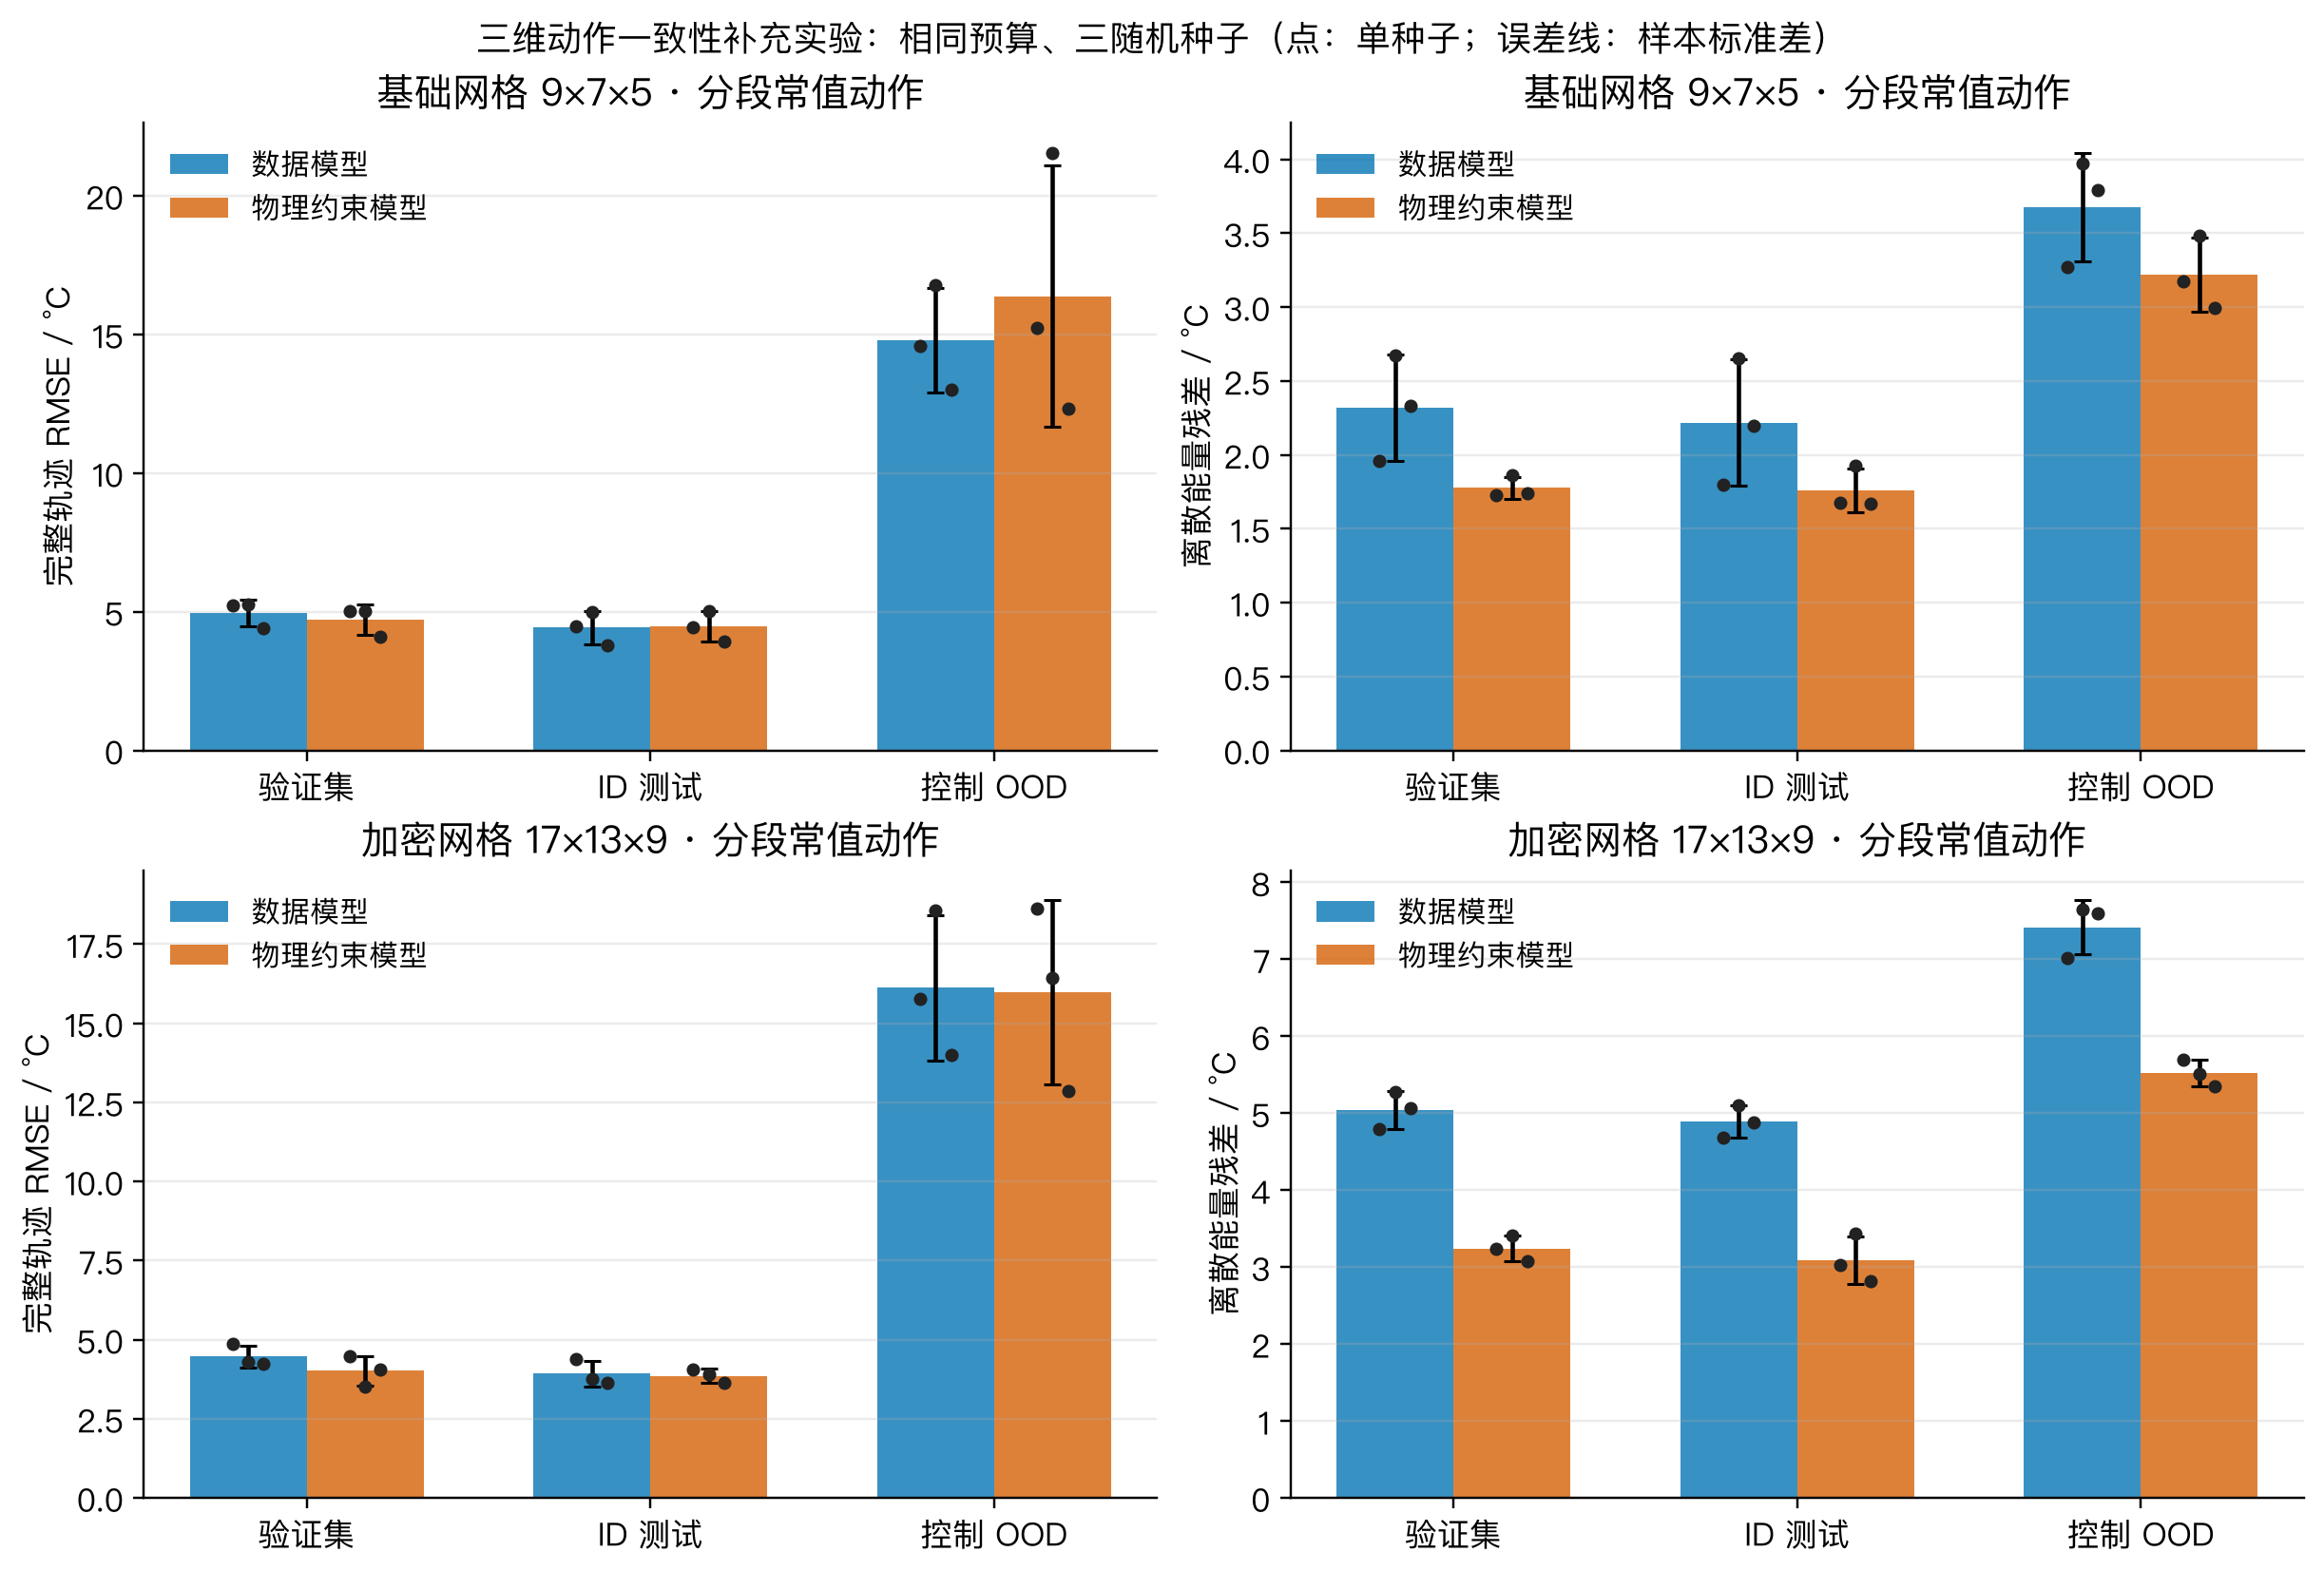
\includegraphics[width=0.98\textwidth]{three_dimensional_zoh_comparison.png}
  \caption{分段常值动作下，两种三维网格的滚动误差与离散能量残差；点表示单种子结果，误差线为样本标准差}
  \label{fig:three_dimensional_replicates}
\end{figure}

\subsection{固定工况的空间温度分布}

图\ref{fig:three_dimensional_cutaway}展示固定ID工况74、$t=\SI{192}{\second}$ 和模型种子42的空间温度分布，以 $25\times19\times13$ 网格的分段常值动作BDF解作为细参考场。每个面板切去朝向观察者的一个八分体，使三个中心切面与外表面同时可见；四面板使用统一色标，学习模型在 $17\times13\times9$ 原生网格上显示，不作显示插值。工况与时刻的选取依据见附录。

将细网格BDF场投影到模型网格后，该时刻显式欧拉、数据模型和物理约束模型的场RMSE分别为 $0.27$、$6.40$ 和 \SI{3.23}{\degreeCelsius}。物理约束模型误差小于数据模型、大于数值基线。该图限于固定案例的空间误差，总体预测性能由全部轨迹统计评价，跨几何泛化仍未检验。相关端淬数字孪生研究关注三维温度场重建，本文评价给定炉温动作下的未来状态递推\cite{midaoui2026jominy}。

\begin{figure}[H]
  \centering
  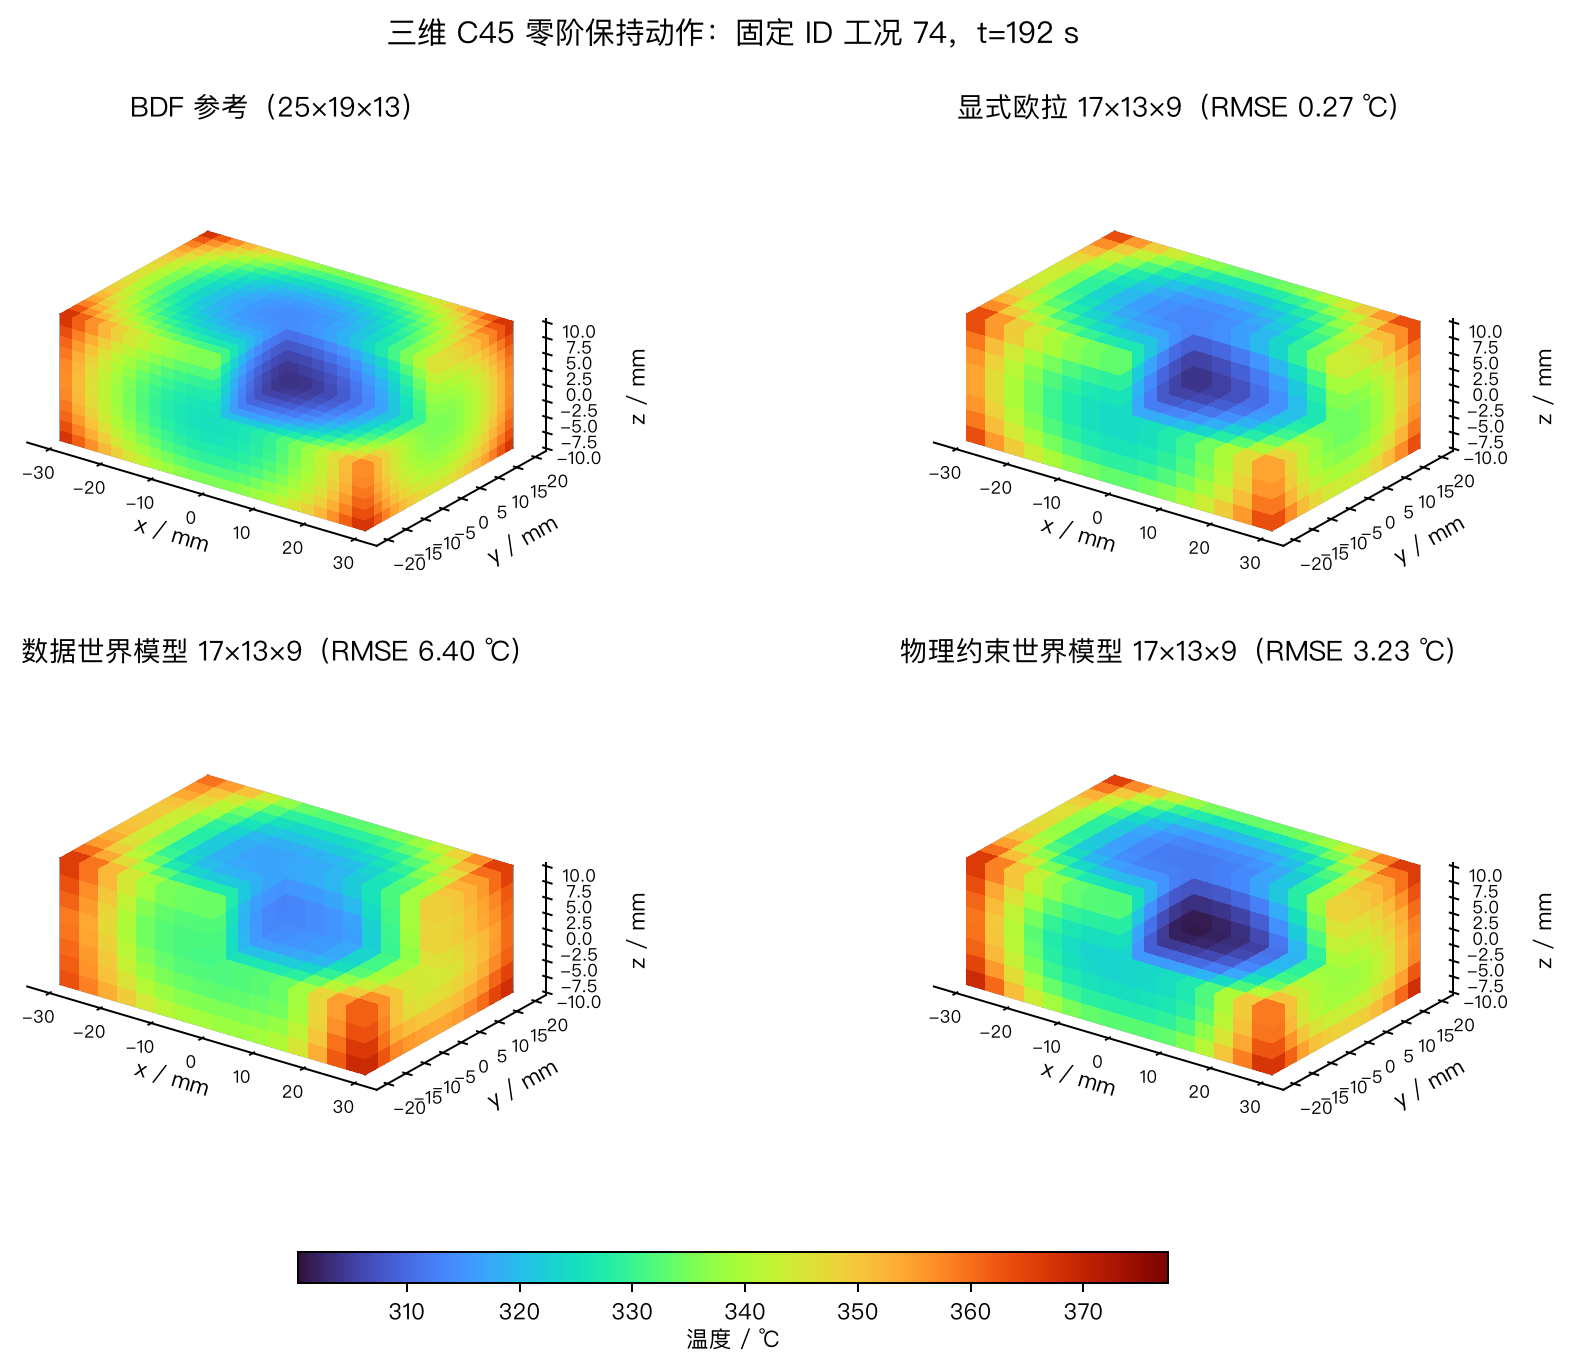
\includegraphics[width=0.95\textwidth]{three_dimensional_temperature_cutaway_zoh.png}
  \caption{分段常值炉温动作下，固定三维C45试块工况的八分体剖视温度场}
  \label{fig:three_dimensional_cutaway}
\end{figure}

物理约束改善了部分参数外推表现与离散一致性，控制曲线及三维 OOD 的稳定精度优势缺乏统计支持。自主 $\Heff$ 的预测收益限于已知动态边界及参考状态训练、验证条件；计时未建立相对低成本数值模型的综合优势。下一章评价有限测温条件下的状态与边界估计及其闭环控制表现。

\chapter{边界辨识、状态估计与闭环控制}

本章研究有限测温、动态边界未知条件下的一维平板炉温控制。世界模型提供温度场预报，因果边界观测器估计等效换热系数，增广状态滤波器联合校正温度场与边界参数。闭环实验评价状态估计精度、测点布局及后验不确定性对炉温决策的影响。

\section{观测条件与评价安排}

本章沿用一维均匀对称受热平板。炉温动作、材料物性尺度、密度、厚度、时间步长和初始均匀温度均已知；在线需要估计的是温度场以及随时间变化的 $h,\varepsilon$。材料与几何参数不和边界参数同时辨识。测量取自表面、近表面及可选的中心位置，两种布局分别为
\begin{equation}
  \mathcal{S}_4=\{0,0.025,0.975,1\},\qquad
  \mathcal{S}_5=\mathcal{S}_4\cup\{0.5\},
  \label{eq:sensor_layouts}
\end{equation}
其中集合元素为归一化位置 $x/L$。四点布局不测中心温度；五点布局含中心热电偶，适用于仪器化试样或内部测温可用的条件。除专门改变测量条件的实验外，观测噪声均为标准差 \SI{0.5}{\degreeCelsius} 的独立高斯噪声。

开环估计使用预先给定的炉温序列，测量用于更新状态和边界，估计结果不改变炉温。闭环控制根据当前估计重新选择动作，后续温度与测量受到控制策略影响。开环重建精度反映给定动作下的估计能力，闭环效果由反馈轨迹上的误差和控制指标评价。

边界反演采用固定步长数值模型生成的 100 条动态轨迹检查反演误差、确定观测窗口；另行生成的 100 条动态留出轨迹用于评价窗口固定后、由观测器驱动的温度递推。集合滤波使用 BDF 轨迹：10 条用于选择滤波参数，另 90 条用于正式开环估计。边界反演与集合滤波数据的生成器和用途不同，分别统计。

闭环评价包含 10 条未用于滤波校准的 ID 场景，以及参数 OOD 的 10 条探索场景和 40 条独立确认场景；后两组互不重叠，承担不同的研究设计角色。涉及世界模型的比较使用种子 42、7、123 对应的三个已训练模型，在各自评价轨迹上不重新选模或调参。三个种子构成固定模型面板，同一物理场景下的重复运行不作为三个独立工况。直接热平衡反演不依赖网络，其参数误差不按三个模型种子重复计数。

控制器和布局的配对比较以每个场景内三个模型的指标均值为统计量，按场景进行 100000 次 bootstrap。回合成功比例描述执行记录；场景全成功要求三个模型在同一场景下均成功，其 Wilson 区间按独立场景数计算。统计结论以当前模型面板和场景抽样假设为条件，不表示对任意重训练模型或工业炉次的保证。

\section{由历史测温估计等效边界}

在单一表面温度或一维对称两侧温度下，式\eqref{eq:heff}将当前瞬时热流写为 $\Heff$ 与边界温差的乘积。净边界热流的估计可用于恢复这一组合。对表面半控制体应用式\eqref{eq:surface_discrete_balance}，利用相邻时刻的表面和近表面温度，有

\begin{equation}
  \widehat{\Heff}_{n-1}
  =\frac{\widehat{q}_{s,n-1}}{\Tinfty_{n-1}-T_{s,n}}.
  \label{eq:heff_observer}
\end{equation}

$\widehat q_{s,n-1}$ 由半隐式离散热平衡反演，分母使用新时刻表面温度 $T_{s,n}$，与表面离散式一致。状态 $n$ 的测量到达后，观测器得到上一转移的边界估计，并将其用于下一次转移；初始转移采用训练范围中点先验。该时序只需要当前及历史测量。

温度差分容易放大测量噪声，因此对边界平衡式采用后向滑动窗口最小二乘。在生成种子为 20260904 的 100 条动态边界轨迹上扫描窗口后，\SI{0.5}{\degreeCelsius} 噪声条件采用30~s窗口；后续留出评价保持该窗口不变。令窗口分母为 $D_n=\sum_j x_j^2$，其中 $x_j$ 与离散边界温差成正比。当 $D_n\leq10^{-12}$ 时，观测器停用比值更新，返回可行区间中点；其余估计截断至训练边界对应的 $\Heff$ 区间。所报告的反演与留出评价中均未触发低激励回退。

在这组窗口选择轨迹上，无噪声单步反演的 $\Heff$ RMSE 为 \SI{0.002}{\watt\per\square\metre\per\kelvin}；加入 \SI{0.5}{\degreeCelsius} 噪声后，采用 30~s 窗口的误差为 \SI{18.45}{\watt\per\square\metre\per\kelvin}。这两个数值描述反演与窗口选择阶段的表现，不作为独立留出误差。窗口平滑减轻差分噪声，同时引入对边界变化的跟踪滞后，与逆热传导问题的噪声敏感性一致\cite{frankel2007loads,chen2019online}。

生成种子为 20260907 的另100条动态边界留出轨迹用于观测器驱动的温度预测：窗口保持固定，因果观测结果作为世界模型的边界输入，温度场通过模型逐步递推，结果见表\ref{tab:causal_heff_observer}。这组轨迹与上一章表\ref{tab:heff_results}的动态留出集相同，表中均值与样本标准差来自三个模型种子。无噪声时的轨迹误差为 \SI{1.608}{\degreeCelsius}，带噪时增至 \SI{10.018}{\degreeCelsius}。热平衡反演在理想测量下能够支持温度递推，差分噪声则随边界输入传入长期预测。表中残差以各自估计的 $\Heff$ 计算，带噪分支残差较低只表示预测与估计边界较为自洽，不能据此认为其温度预测或真实物理一致性更好。

\begin{table}[H]
  \centering
  \caption{因果边界观测驱动的温度递推，均值$\pm$样本标准差}
  \label{tab:causal_heff_observer}
  \begin{tabular}{lcc}
    \toprule
    测量条件 & 滚动 RMSE/\si{\degreeCelsius} & 估计边界下的残差/\si{\degreeCelsius} \\
    \midrule
    无噪声因果观测 & $1.608\pm0.103$ & $17.37\pm2.78$ \\
    \SI{0.5}{\degreeCelsius} 噪声因果观测 & $10.018\pm0.112$ & $16.40\pm2.76$ \\
    \bottomrule
  \end{tabular}
\end{table}

图\ref{fig:heff_deployment}将因果观测与参考边界输入并列展示。图中的真实 $\Heff$ 由参考表面温度构造，包含额外状态信息，不能用来单独识别参数表示的收益；同信息的自主边界表示比较见表\ref{tab:heff_results}。图\ref{fig:heff_trajectory}取模型种子 42，在联合边界类别内按参考状态条件 $\Heff$ 模型的 RMSE 最接近类别中位数选取轨迹，用于显示边界跟踪和温度误差的对应关系。

\begin{figure}[H]
  \centering
  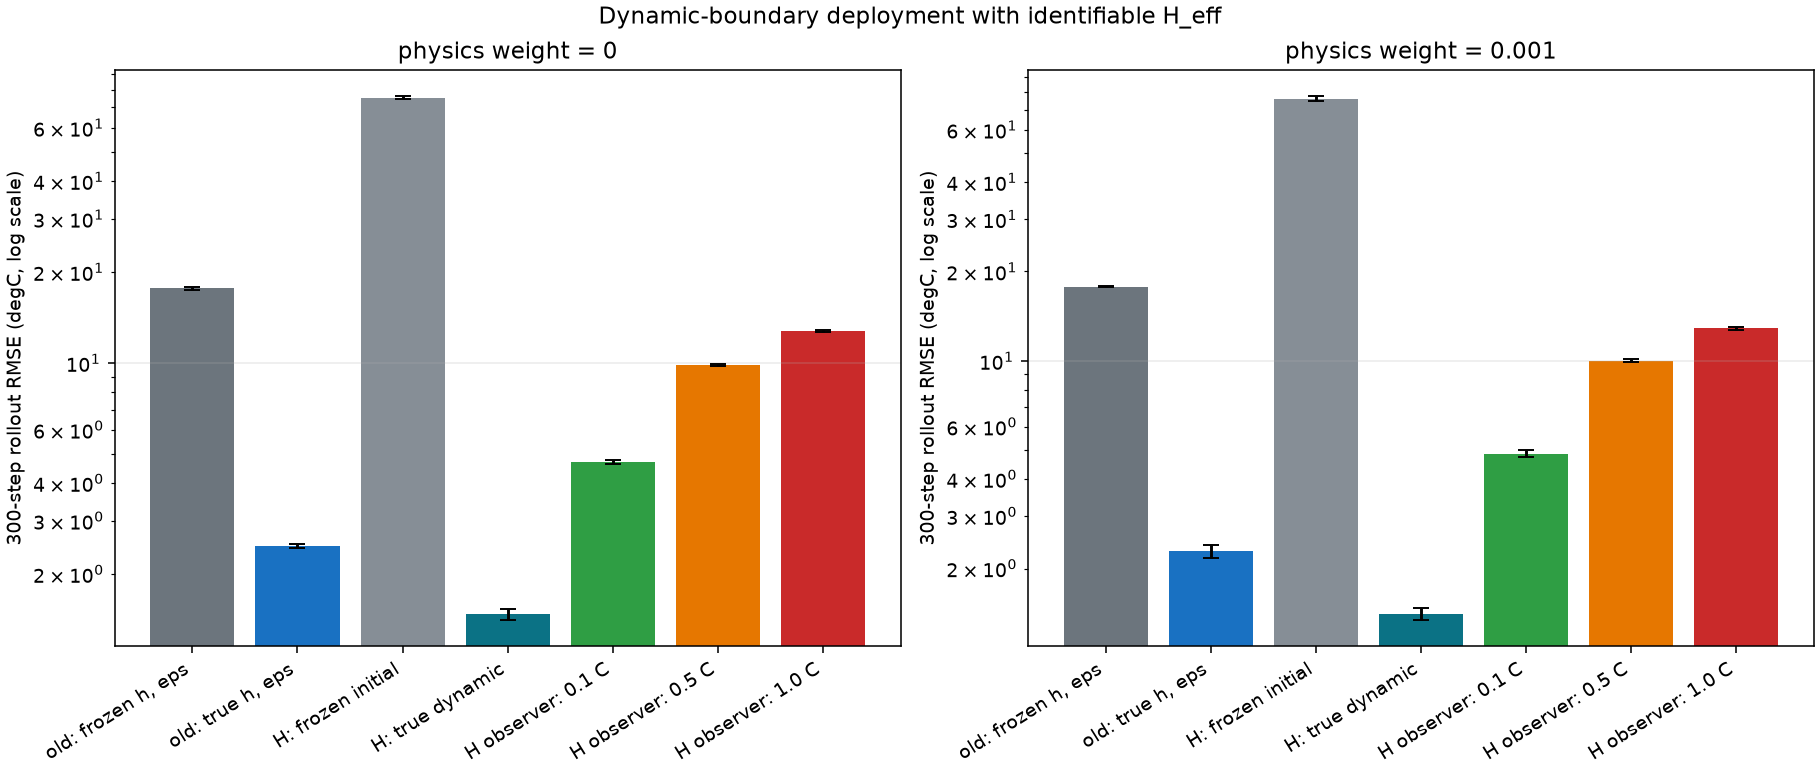
\includegraphics[width=0.96\textwidth]{deployment_comparison.png}
  \caption{参考状态条件边界输入与因果观测方式的比较；同信息自主滚动结果见表\ref{tab:heff_results}}
  \label{fig:heff_deployment}
\end{figure}

\begin{figure}[H]
  \centering
  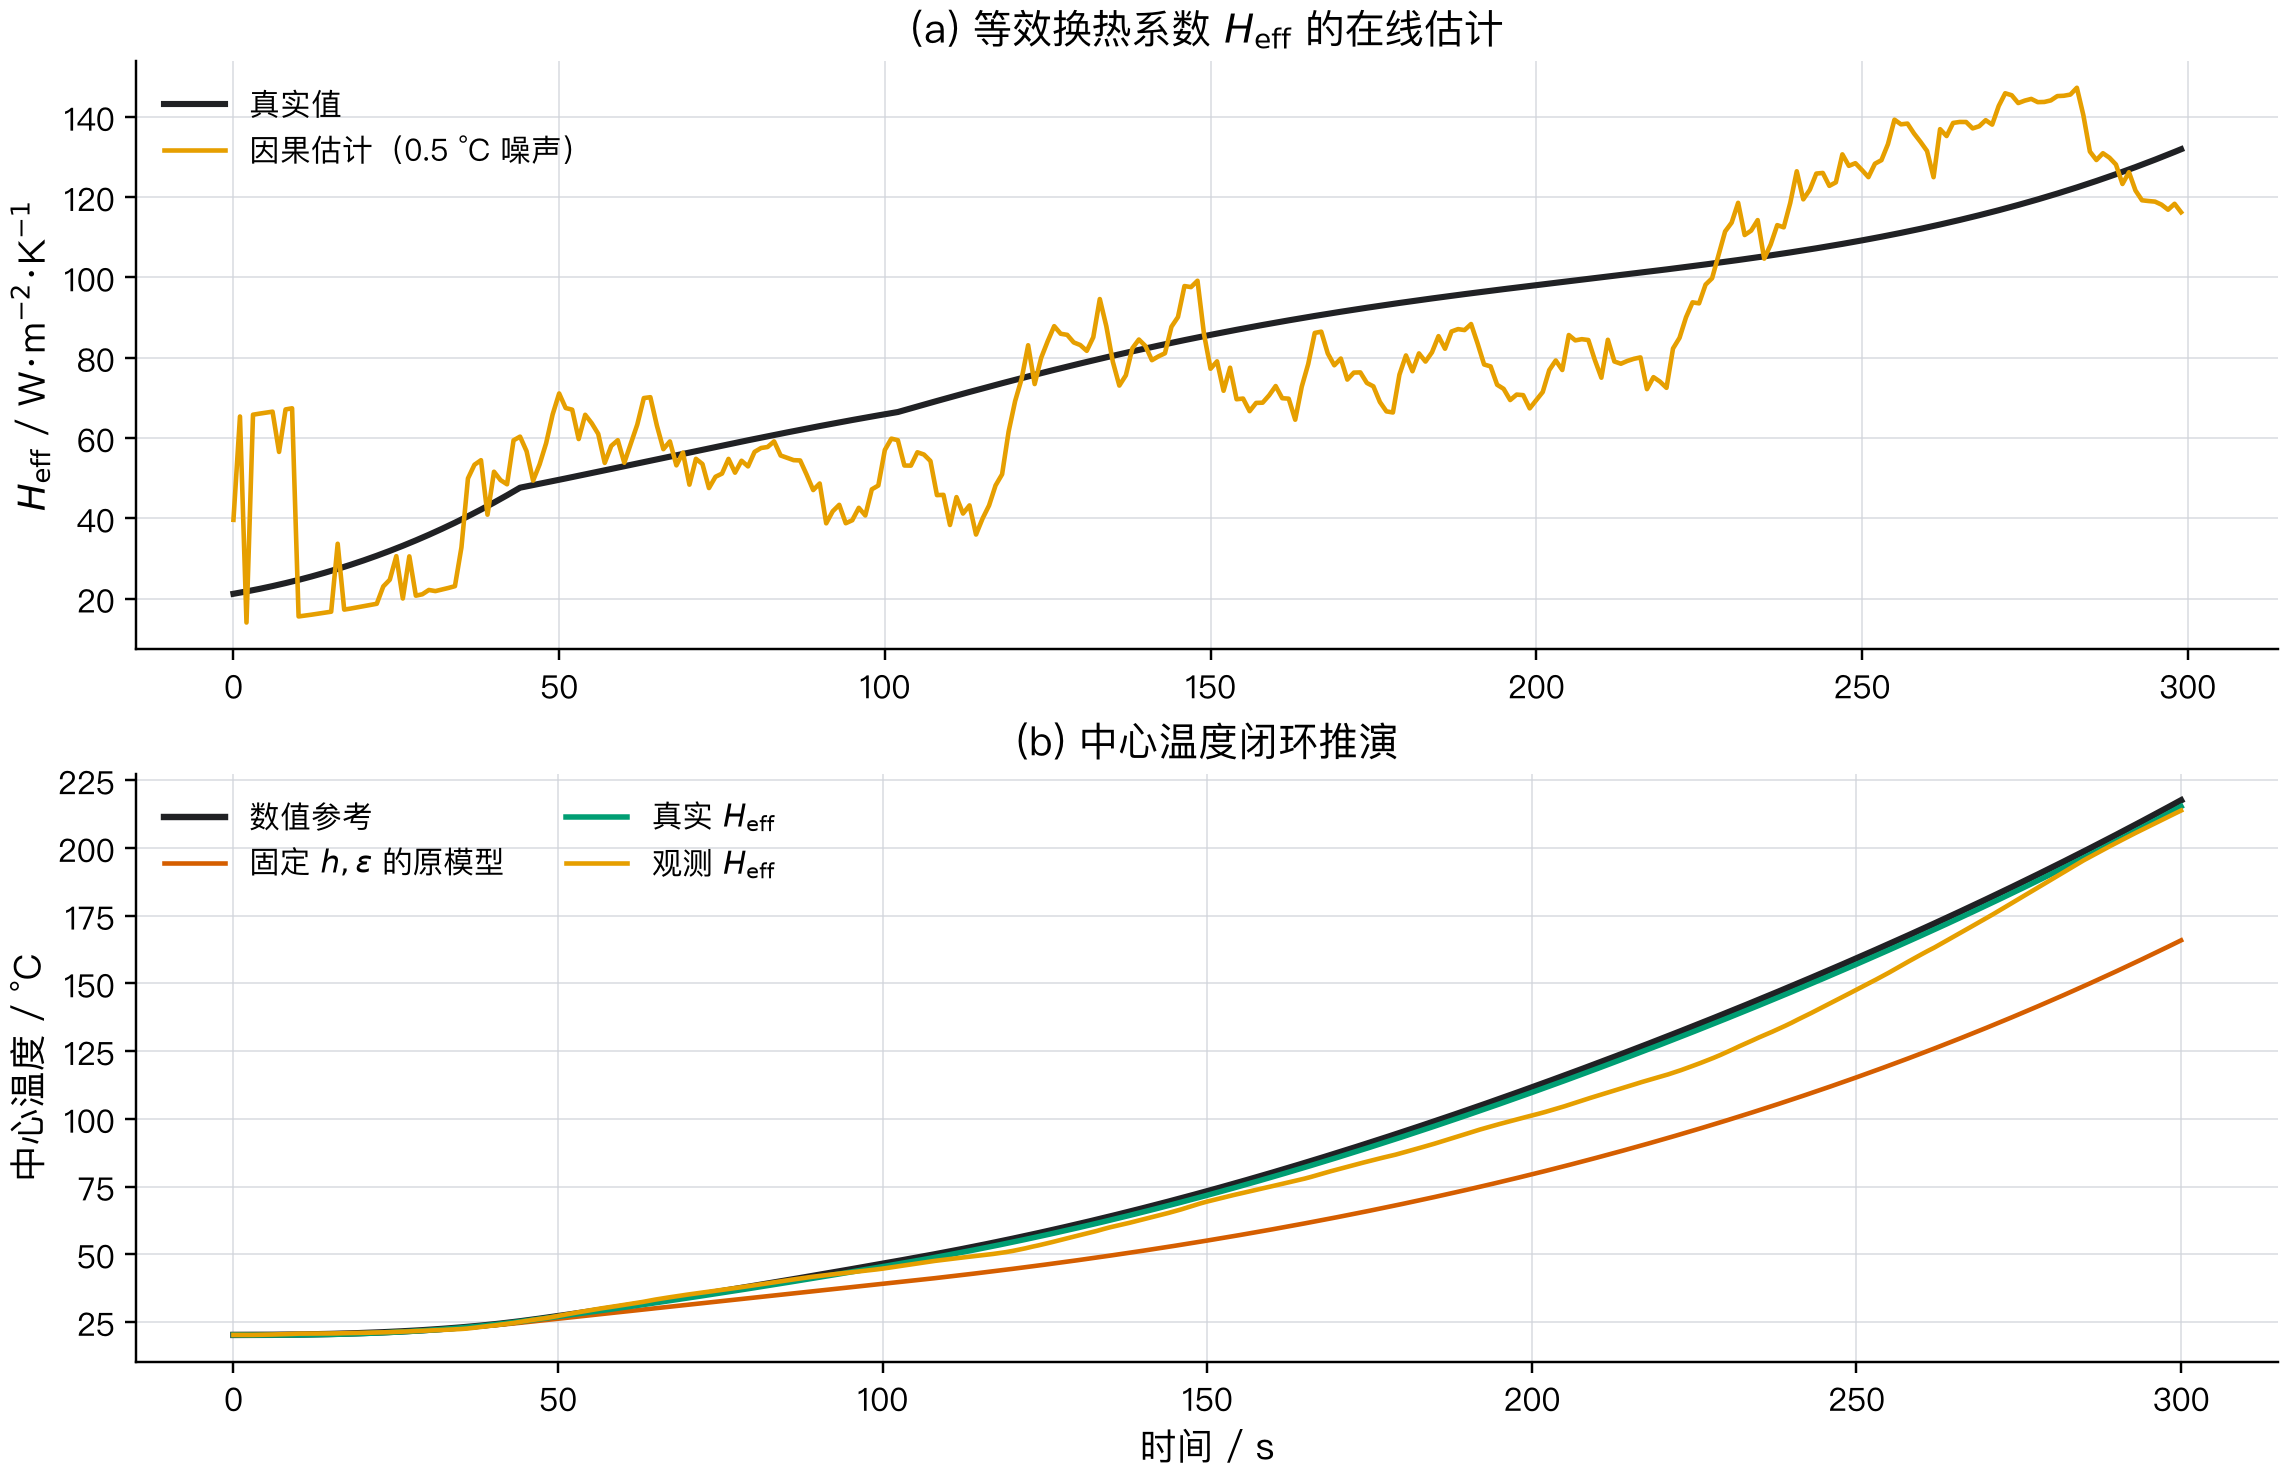
\includegraphics[width=0.96\textwidth]{effective_boundary_trajectory_zh.png}
  \caption{等效换热系数因果观测及给定炉温序列下的递推（真实有效边界采用参考状态条件输入）}
  \label{fig:heff_trajectory}
\end{figure}

图中“闭环推演”指给定炉温序列下的状态递推，不含炉温反馈决策。因果观测能够跟踪边界的主要变化，带噪结果表明仅更新边界输入不足以保持全场精度。集合滤波将稀疏温度测量同时用于温度场和边界参数的校正。

\section{稀疏测温下的温度场重建}

\subsection{增广状态滤波与测点布局}

本文采用 DEnKF，即确定性集合卡尔曼滤波（deterministic ensemble Kalman filter）\cite{evensen2009enkf,oka2020enkf}。温度节点与边界参数组成增广状态
\begin{equation}
  \bm{z}_n=[T_1^n,\ldots,T_{41}^n,h_n,\varepsilon_n]^{\mathsf T}.
\end{equation}
64 个集合成员分别经过世界模型预报，并通过式\eqref{eq:heff}生成各自的有效边界输入。测量更新利用温度状态、边界参数与测点温度之间的样本交叉协方差进行联合校正；温度场同时保持本研究的中心面对称条件。配置见表\ref{tab:enkf_config}。这里对 $h,\varepsilon$ 的分解受到动态先验、参数支持域和历史观测共同约束，不表示从单次瞬时热流就能唯一识别两者。

\begin{table}[H]
  \centering
  \caption{增广状态集合滤波配置}
  \label{tab:enkf_config}
  \begin{tabular}{lc@{\qquad}lc}
    \toprule
    参数 & 数值 & 参数 & 数值 \\
    \midrule
    集合规模 & 64 & 测温噪声标准差 & \SI{0.5}{\degreeCelsius} \\
    初始温度场标准差 & \SI{0.25}{\degreeCelsius} & 温度状态过程噪声 & \SI{0.03}{\degreeCelsius} \\
    $h$ 初始先验 & $35\pm12$~\si{\watt\per\square\metre\per\kelvin} & $h$ 过程噪声 & \SI{1.0}{\watt\per\square\metre\per\kelvin} \\
    $\varepsilon$ 初始先验 & $0.775\pm0.070$ & $\varepsilon$ 过程噪声 & 0.004 \\
    集合膨胀系数 & 1.01 & 局部化半径 & 8 个节点 \\
    \bottomrule
  \end{tabular}
\end{table}

区间由集合成员的 5\% 和 95\% 分位数构成。未测节点覆盖率统计除初始状态外、参考温度落入该区间的节点--时刻比例；$h,\varepsilon$ 的覆盖率按全部参数时刻统计。90 条开环评价轨迹与三个模型共形成 270 条模型--场景记录，测点布局比较见表\ref{tab:sensor_layout}。

\begin{table}[H]
  \centering
  \caption{稀疏测点布局的温度场重建结果，RMSE 单位：\si{\degreeCelsius}}
  \label{tab:sensor_layout}
  \small
  \resizebox{\textwidth}{!}{%
  \begin{tabular}{lcccc}
    \toprule
    传感器布局 & \shortstack{全场\\RMSE} & \shortstack{未测节点\\RMSE} & \shortstack{中心\\RMSE} & \shortstack{未测节点\\90\% 覆盖率} \\
    \midrule
    无中心测点的近表面 4 点 & 2.022 & 2.128 & 2.854 & $81.5\%$ \\
    含中心热电偶的理想 5 点 & 1.008 & 1.073 & 0.231 & $90.8\%$ \\
    \bottomrule
  \end{tabular}}
\end{table}

四点布局的未测节点 RMSE 为 \SI{2.128}{\degreeCelsius}，中心 RMSE 为 \SI{2.854}{\degreeCelsius}。五点布局的相应误差更低，但 \SI{0.231}{\degreeCelsius} 的中心 RMSE 包含直接中心测量的校正效果，不能解释为仅由表面温度推断心部的精度。两种布局各自未测节点集合也不同。有限测点下的重建能力必须连同测点位置解释，这与已有温度场重建研究的结论一致\cite{liu2022reconstruction}。图\ref{fig:assimilation}给出五点条件下的温度场与边界同化结果。

\begin{figure}[H]
  \centering
  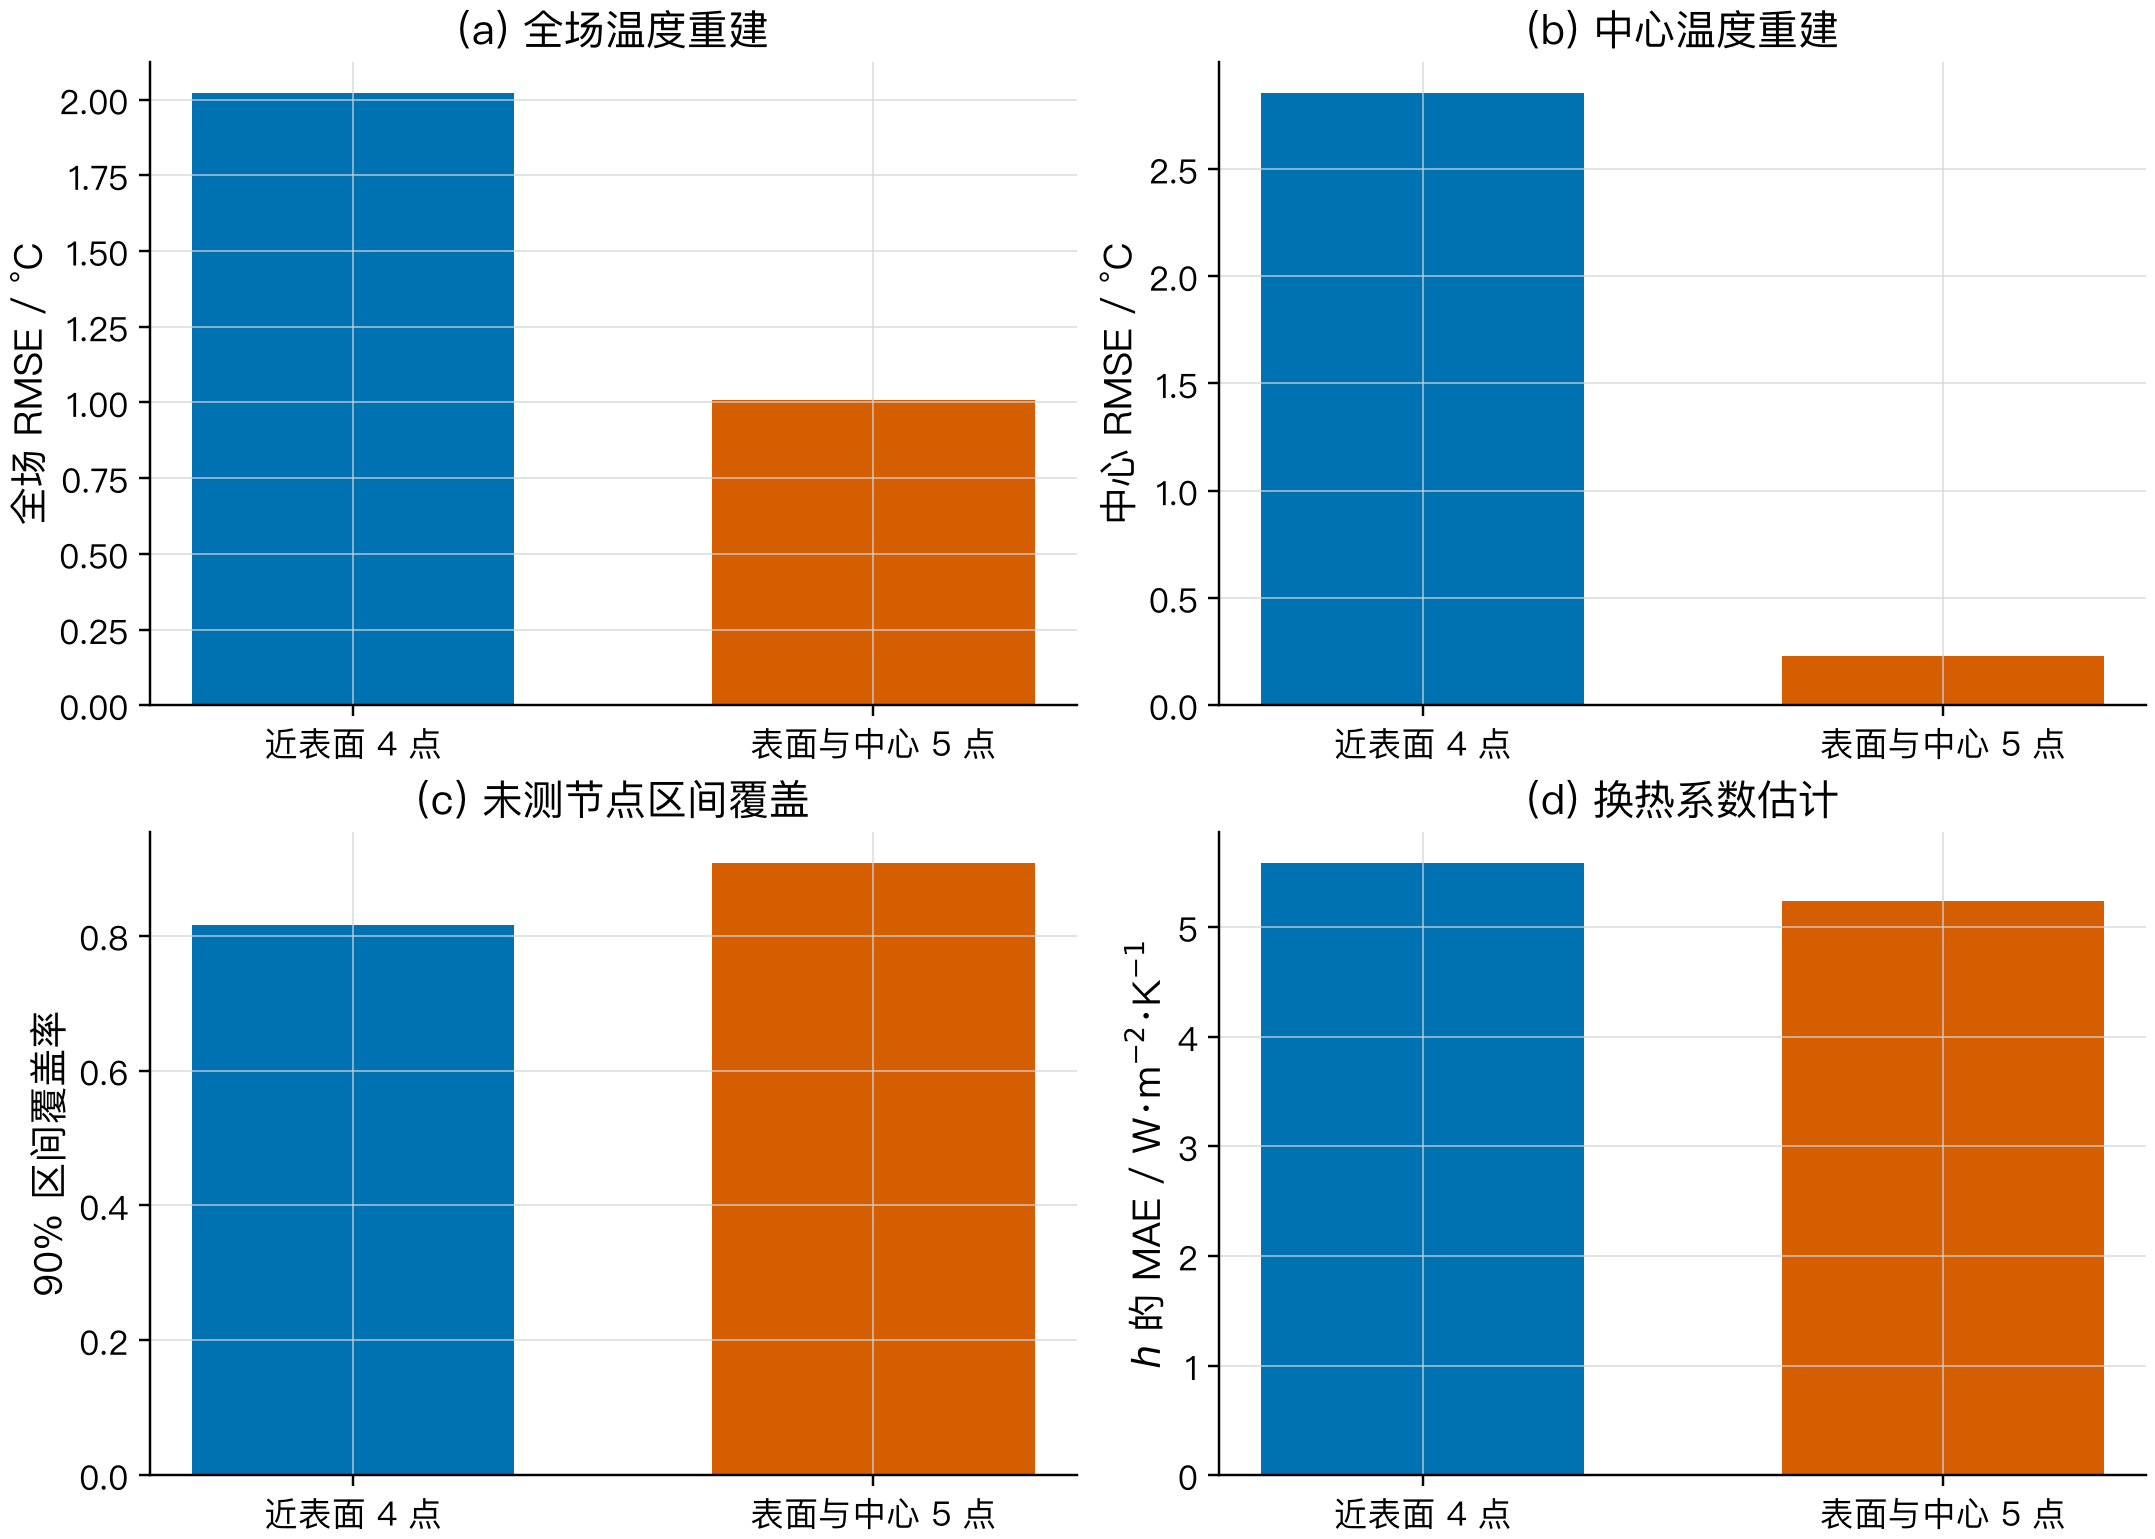
\includegraphics[width=0.96\textwidth]{open_loop_assimilation.png}
  \caption{五点测温条件下的温度场与边界参数同化结果}
  \label{fig:assimilation}
\end{figure}

参数支持域同样影响估计。在五点参数 OOD 评价中，沿用训练范围截断后验时，全场 RMSE 为 \SI{5.247}{\degreeCelsius}。将支持域扩展为 $h\in[5,80]$~\si{\watt\per\square\metre\per\kelvin}、$\varepsilon\in[0.45,0.98]$，同时把初始先验标准差从 12、0.070 分别增至 15、0.100 后，全场 RMSE 降至 \SI{2.813}{\degreeCelsius}，中心 RMSE 为 \SI{0.290}{\degreeCelsius}，两种参数的 90\% 区间覆盖率分别为 $79.9\%$ 和 $76.5\%$。该比较支持扩大支持域与先验不确定性的整体配置，未单独识别其中某一项的贡献。

\subsection{测量噪声与传感器响应}

测量噪声与响应迟滞在四点布局下分别评价：改变噪声标准差，并用一阶响应生成滞后测温。每个条件包含 90 条 BDF 轨迹和三个模型，滤波器统一按瞬时测量处理。结果见表\ref{tab:sensor_robustness}与图\ref{fig:sensor_robustness}。

\begin{table}[H]
  \centering
  \caption{近表面四点测温的噪声与响应滞后结果}
  \label{tab:sensor_robustness}
  \resizebox{\textwidth}{!}{%
  \begin{tabular}{lccc}
    \toprule
    测量条件 & 未测节点 RMSE/\si{\degreeCelsius} & 中心 RMSE/\si{\degreeCelsius} & 90\% 覆盖率 \\
    \midrule
    噪声 \SI{0.2}{\degreeCelsius} & 2.297 & 2.985 & $73.9\%$ \\
    噪声 \SI{0.5}{\degreeCelsius} & 2.128 & 2.854 & $81.5\%$ \\
    噪声 \SI{1.0}{\degreeCelsius} & 2.100 & 2.853 & $86.0\%$ \\
    \SI{2}{\second} 响应时间常数，噪声 \SI{0.5}{\degreeCelsius} & 2.691 & 3.433 & $65.2\%$ \\
    \SI{5}{\second} 响应时间常数，噪声 \SI{0.5}{\degreeCelsius} & 4.894 & 5.501 & $34.4\%$ \\
    \bottomrule
  \end{tabular}}
\end{table}

噪声标准差从 \SI{0.2}{\degreeCelsius} 增至 \SI{1.0}{\degreeCelsius} 时，RMSE 没有明显恶化，区间覆盖率随之上升。观测协方差按实际噪声同步设置，噪声增大也降低了滤波器对局部测量的权重，结果不能解释为增加噪声具有一般收益。忽略响应迟滞时，时间常数为 \SI{5}{\second} 的未测节点 RMSE 增至 \SI{4.894}{\degreeCelsius}，覆盖率降至 $34.4\%$。误差增加与覆盖率下降对应观测方程和测量动态的不匹配。

\begin{figure}[H]
  \centering
  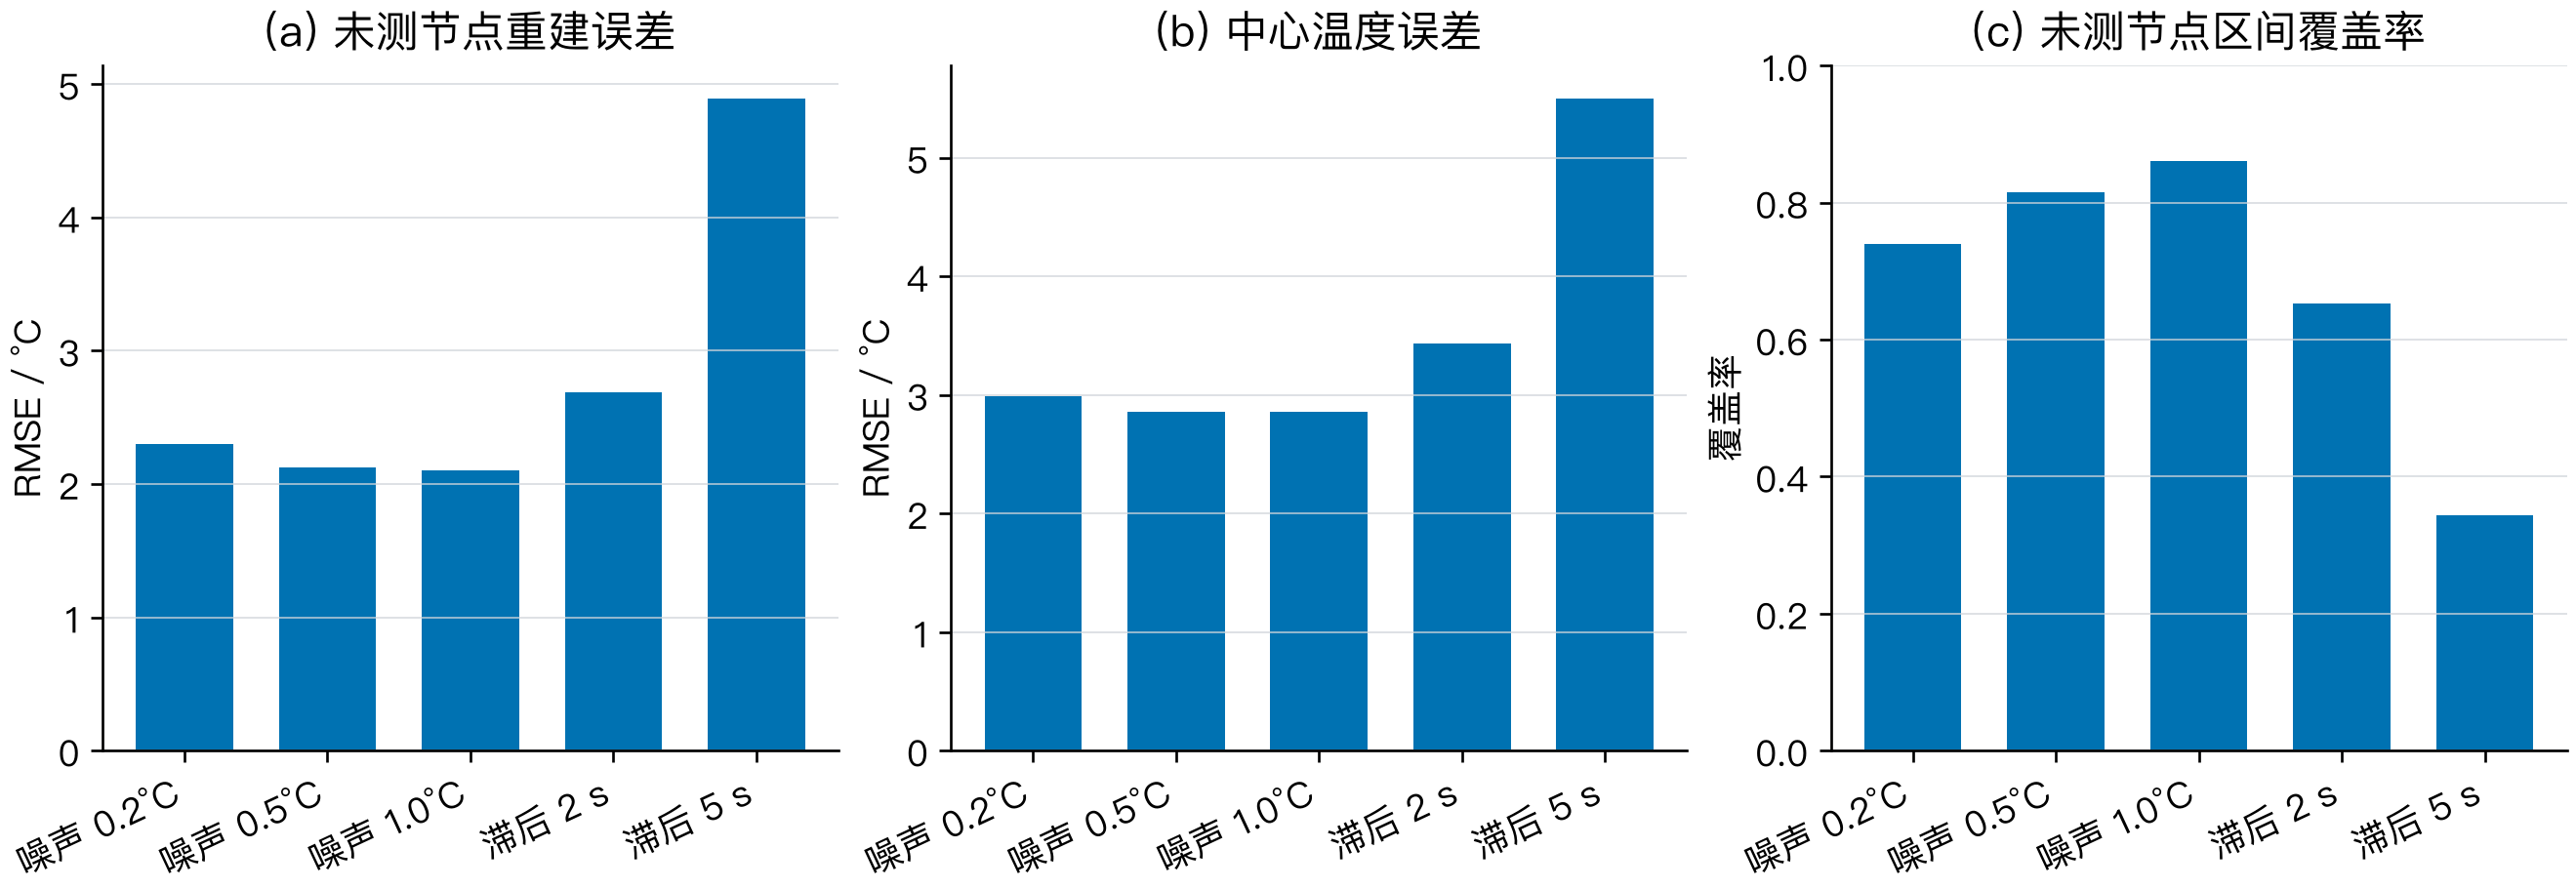
\includegraphics[width=0.96\textwidth]{sensor_robustness.png}
  \caption{近表面稀疏测温对随机噪声与传感器响应滞后的鲁棒性}
  \label{fig:sensor_robustness}
\end{figure}

为匹配观测动态，在增广状态中增加四个传感器响应状态 $r_{j,n}$：

\begin{equation}
  r_{j,n+1}=\alpha r_{j,n}+(1-\alpha)T_{i_j,n+1},\qquad
  y_{j,n+1}=r_{j,n+1}+v_{j,n+1},\qquad
  \alpha=\exp(-\Delta t/\tau_s).
  \label{eq:sensor_response}
\end{equation}

其中 $i_j$ 为测点节点，$\tau_s$ 为响应时间常数，$v_{j,n}$ 的标准差为 \SI{0.5}{\degreeCelsius}。递推采用采样区间内温度取右端值的分段常数近似，初始传感器温度与工件平衡，与迟滞试验的生成方式一致。预报阶段以推演得到的工件温度更新响应状态；同化阶段以响应状态预测测量，并通过交叉协方差校正温度场与边界。该过程只使用已经到达的测量。

真实时间常数预先固定为 2 s 和 5 s。校准使用集合滤波的10条独立校准轨迹及已知测点真温度，在 0--8 s、间隔 0.1 s 的候选网格上最小化响应预测与带噪测量的平方误差，分别选中 2.0 s 和 5.0 s 后固定。该仪器化标定以独立温度参照为前提，未检验从未知工件温度同时识别传感器和边界的能力。

瞬时观测与响应状态两种滤波器共用模型、测量序列、初始随机数及过程噪声；集合规模、局部化、膨胀和边界先验保持一致。两种响应条件、两种滤波器、90 条评价轨迹与三个模型共形成 1080 条记录，其中瞬时观测分支的 540 条记录与前述迟滞试验逐项一致。表\ref{tab:sensor_response}给出留出结果。

\begin{table}[H]
  \centering
  \caption{响应状态补偿的留出轨迹结果，每行 90 条轨迹、三个模型种子}
  \label{tab:sensor_response}
  \small
  \begin{tabular}{clrrrr}
    \toprule
    $\tau_s$/s & 观测模型 & \shortstack{未测节点\\RMSE/°C} & \shortstack{中心\\RMSE/°C} & \shortstack{90\% 区间\\覆盖率} & \shortstack{区间平均\\宽度/°C} \\
    \midrule
    2 & 瞬时观测 & 2.691 & 3.433 & $65.2\%$ & 5.382 \\
    2 & 响应状态 & 2.147 & 2.881 & $82.5\%$ & 5.567 \\
    5 & 瞬时观测 & 4.894 & 5.501 & $34.4\%$ & 5.384 \\
    5 & 响应状态 & 2.178 & 2.932 & $84.2\%$ & 5.931 \\
    \bottomrule
  \end{tabular}
\end{table}

轨迹配对结果显示，2 s 条件的未测节点 RMSE 差为 \SI{-0.544}{\degreeCelsius}，95\% 区间为 $[-0.692,-0.394]$~\si{\degreeCelsius}。5 s 条件的配对差为 \SI{-2.716}{\degreeCelsius}，区间为 $[-3.095,-2.342]$~\si{\degreeCelsius}。5 s 条件的误差降低 $55.5\%$，覆盖率提高约 49.8 个百分点，区间平均宽度增加 \SI{0.546}{\degreeCelsius}。响应状态补偿同时降低点估计误差、提高区间覆盖率，支持其减轻迟滞偏差的作用。

\begin{figure}[H]
  \centering
  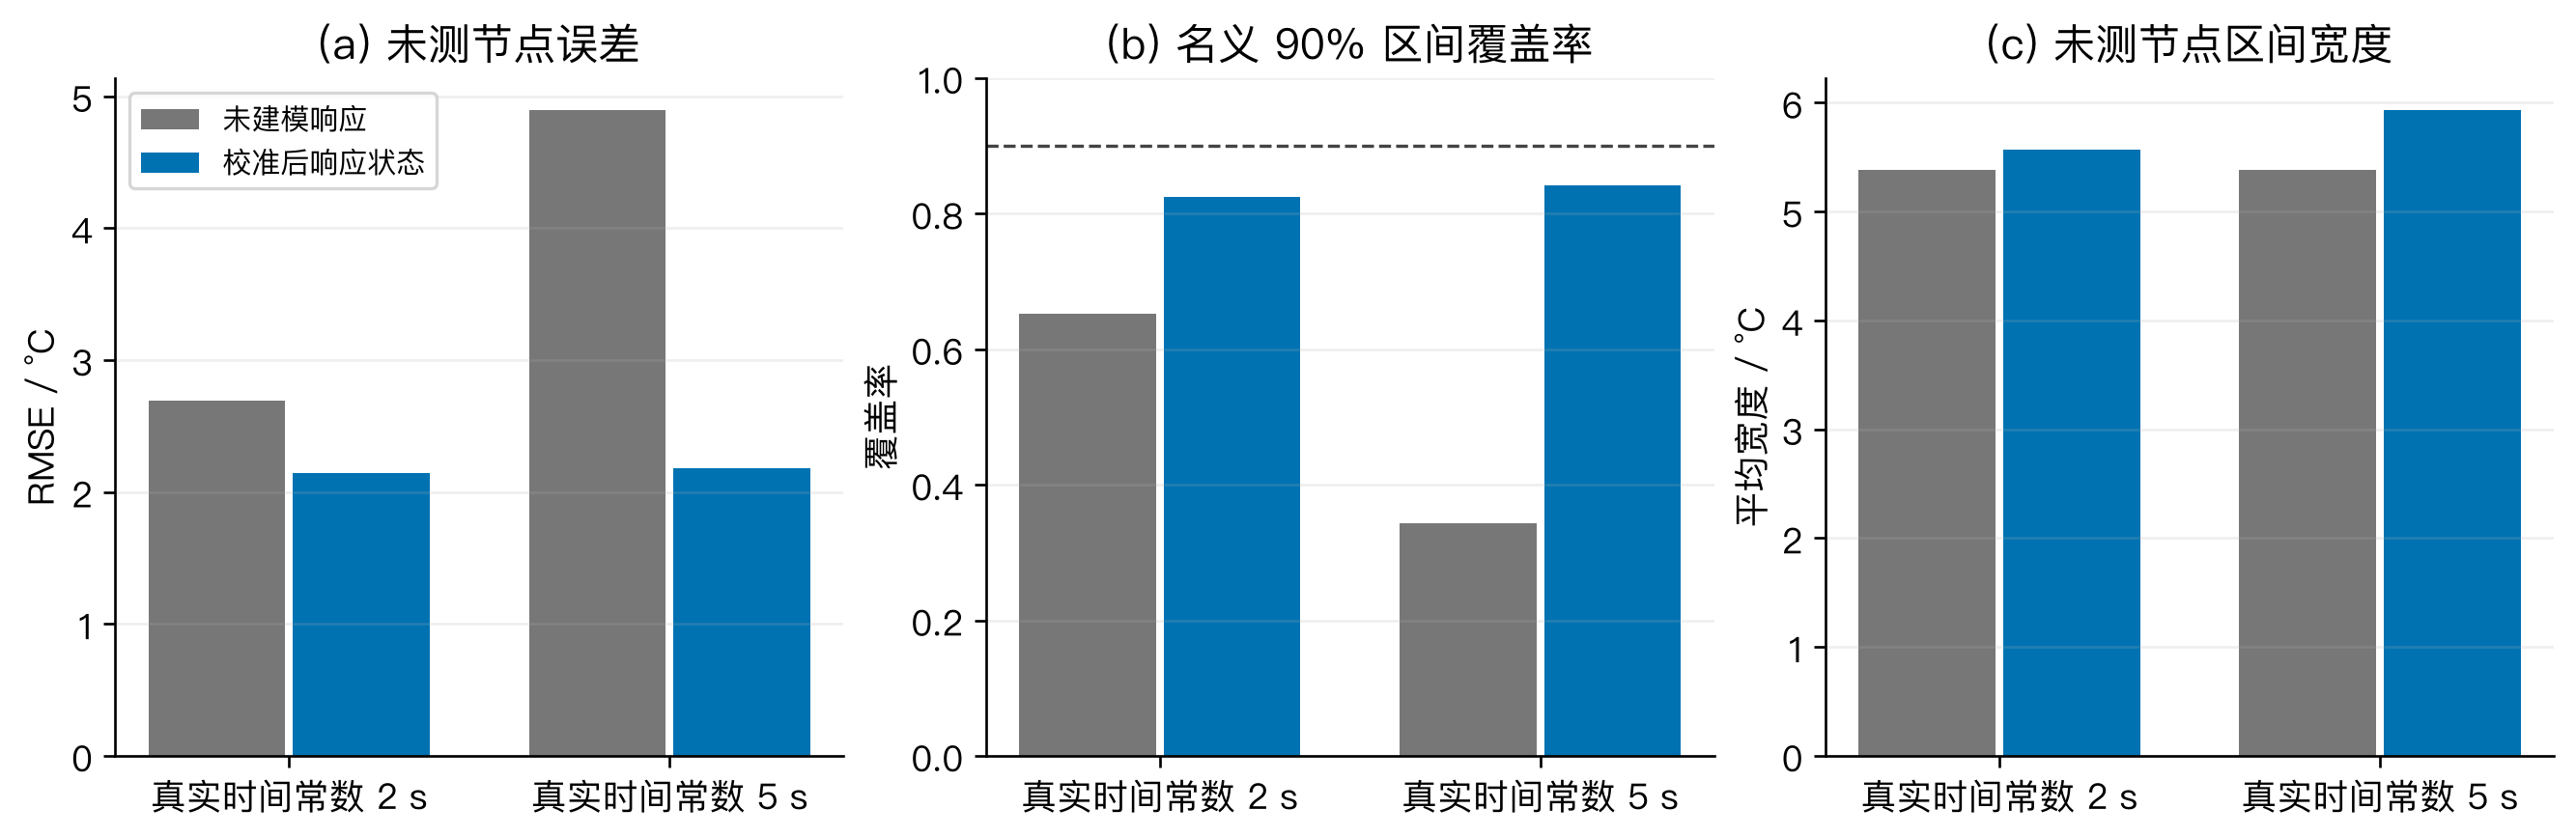
\includegraphics[width=0.98\textwidth]{sensor_response.png}
  \caption{独立校准的传感器响应状态对误差及区间质量的影响}
  \label{fig:sensor_response}
\end{figure}

补偿后的未测节点误差接近无滞后基准，但 $82.5\%$--$84.2\%$ 的覆盖率仍低于名义 $90\%$。证据限于合成一阶传感器及独立响应标定可用的开环估计，未覆盖时间常数漂移、测点响应差异或真实校准误差。后续闭环实验使用无响应滞后的合成测量，不能把本节的补偿收益直接归入闭环控制结果。

\section{共同闭环策略与信息对照}

控制器每 20~s 根据当前状态选择一次炉温，在总长 300~s 的任务内跟踪 \SI{350}{\degreeCelsius} 的中心目标。候选炉温为 $\{300,400,500,600,700,800,900,950\}$~\si{\degreeCelsius}。每个候选值在剩余预测时域内保持常数，选定后只执行首个 20~s 区间，再利用新的观测更新状态。该控制器采用常值尾部的单移动阻塞 MPC，搜索变量仅为当前炉温值。目标温度和约束用于检验控制链路，不构成完整的 C45 工业热处理制度。

所有对照使用相同的候选动作目标函数：

\begin{equation}
  J=|T_c^{\mathrm{end}}-T^*|
  +0.25\Delta T^{\mathrm{end}}
  +5\max(0,T_s^{\max}-T_{\mathrm{lim}})
  +5E+0.01V,
  \label{eq:control_objective}
\end{equation}

其中 $\Delta T^{\mathrm{end}}=\max_i T_i^{\mathrm{end}}-\min_i T_i^{\mathrm{end}}$，$T_s^{\max}$ 为预测时域内两侧表面的最高温度，$E=(a-20)/(950-20)$ 为归一化炉温项，$V=|a-a_{\mathrm{prev}}|$ 为本次动作变化。表面温度上限 $T_{\mathrm{lim}}$ 在 ID 任务中为 \SI{550}{\degreeCelsius}，在参数 OOD 压力测试中收紧至 \SI{360}{\degreeCelsius}。超温通过代价惩罚处理，并非优化器强制满足的硬约束；归一化炉温项也不等同于实测能耗。

执行完回合后，以实际温度和动作轨迹计算综合目标

\begin{equation}
  J_{\mathrm{ep}}=|T_c^{\mathrm{end}}-T^*|
  +0.25\Delta T^{\mathrm{end}}+5O+5\overline{E}+0.01V_{\mathrm{ep}},
  \label{eq:episode_control_objective}
\end{equation}

其中 $O=\max(0,\max_{n,s}T_{s,n}-T_{\mathrm{lim}})$，$\overline E$ 为 300 个执行时刻的归一化炉温均值，$V_{\mathrm{ep}}=|a_1-300|+\sum_{k=2}^{N_{\mathrm{dec}}}|a_k-a_{k-1}|$ 为决策序列总变差，$N_{\mathrm{dec}}$ 为决策次数。表中的“中心误差”指终点中心绝对误差，“平均超温”指各回合峰值超温量 $O$ 的平均。终点中心误差不超过 \SI{10}{\degreeCelsius} 且 $O=0$ 时，记为成功回合\cite{rawlings2017mpc}。

四种控制器使用不同的状态与边界信息。完整状态与真实边界控制器获得完整真实温度场和剩余时域的真实 $h,\varepsilon$ 序列；稀疏状态与真实边界控制器使用滤波温度场估计，未来边界仍已知。两者构成区分状态误差和边界不确定性影响的理想信息对照。后验均值控制由当前测量驱动，使用滤波均值，并将当前 $h,\varepsilon$ 估计保持至预测末端；风险分位控制使用 16 个后验成员，按候选代价的 90\% 分位选择动作\cite{moehle2021risk}。

这两种后验控制在规划中都不读取未来真实边界，也不传播未来边界过程噪声。风险分位数因此描述当前后验、固定参数预测假设下的代价差异，不能解释为表面超温概率保证。候选炉温改变时，辐射基函数也随之改变，必须用每个成员的 $h,\varepsilon$ 和预测表面温度重新计算 $\Heff$。单一的当前 $\Heff$ 只约束既定状态与动作的瞬时热流；其离散转移充分性限于第三章所述冻结旧状态系数的格式，不能替代候选动作下的参数后验。

\section{ID 跟踪与测点布局的闭环影响}

\subsection{理想信息基准与五点测温}

世界模型与 BDF 的动作搜索在 10 条动态边界场景上比较。两者使用相同的代价、候选动作与预测时域，每次决策均获得各自网格上的完整真实状态和全部未来真实边界，仅更换预测动力学及对应网格。世界模型的三个种子共运行 30 个回合，终点中心误差为 \SI{2.096}{\degreeCelsius}，30/30 个回合成功，对应 10/10 个场景全成功及 $[72.2\%,100\%]$ 的95\% Wilson 区间。BDF 搜索在 10/10 个场景成功，终点误差为 \SI{2.120}{\degreeCelsius}。

这一理想条件下，每回合候选规划时间分别为 \SI{0.099}{\second} 与 \SI{6.258}{\second}，比值为 63.4。该计时只对应完整真实状态和未来边界已知的候选动作搜索，任务与表\ref{tab:fair_timing}的完整轨迹推演不同，不能合并为统一速度结论。若仅将边界输入改为 \SI{0.5}{\degreeCelsius} 噪声下的因果观测、仍保留完整真实状态，终点误差为 \SI{3.906}{\degreeCelsius}，成功回合为28/30，场景全成功为9/10，95\%区间为 $[59.6\%,98.2\%]$。这一对照尚未包含由稀疏测温恢复全场的误差。

\begin{figure}[H]
  \centering
  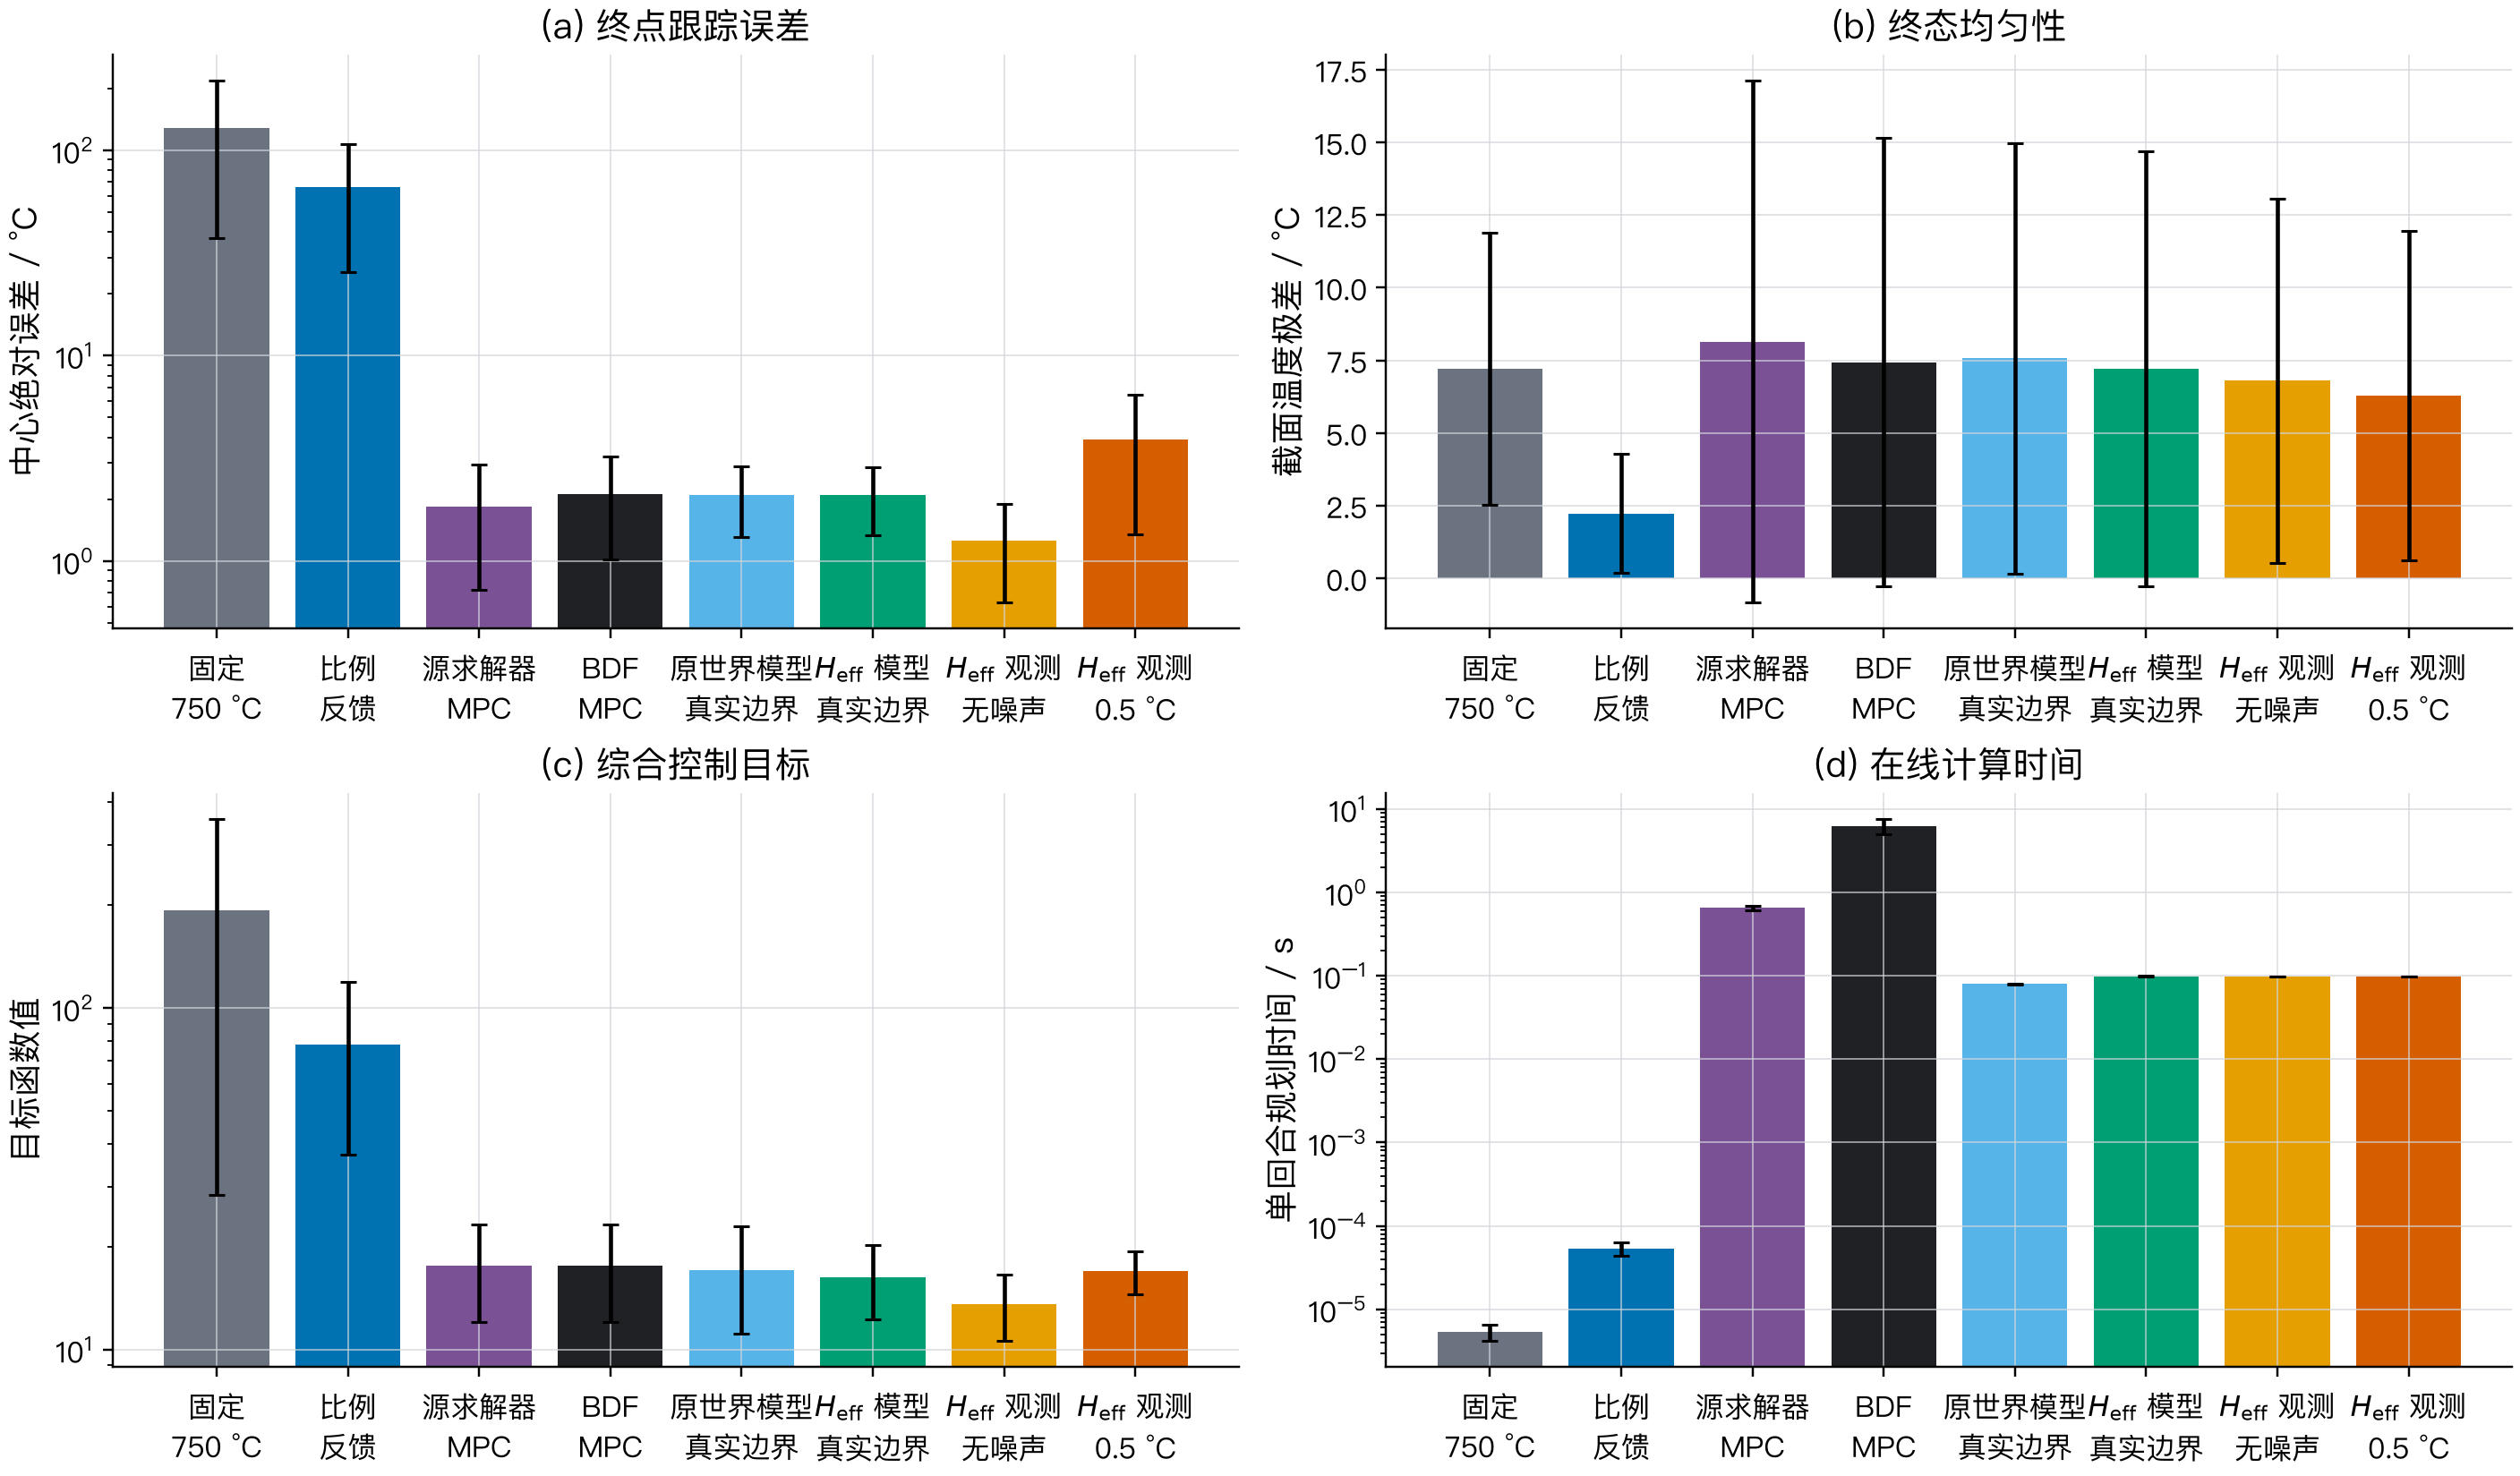
\includegraphics[width=0.96\textwidth]{closed_loop_control_summary.png}
  \caption{完整状态输入下的动态边界滚动动作搜索；真实边界分支获得全部未来边界}
  \label{fig:closed_loop}
\end{figure}

图\ref{fig:closed_loop_trajectory}取模型种子 42 和联合边界轨迹 12。固定炉温产生目标过冲，比例反馈在后段升温不足，BDF 与世界模型动作搜索的终点温度均接近目标。这一代表性轨迹用于说明动作选择的作用，整体判断以场景统计为准。

\begin{figure}[H]
  \centering
  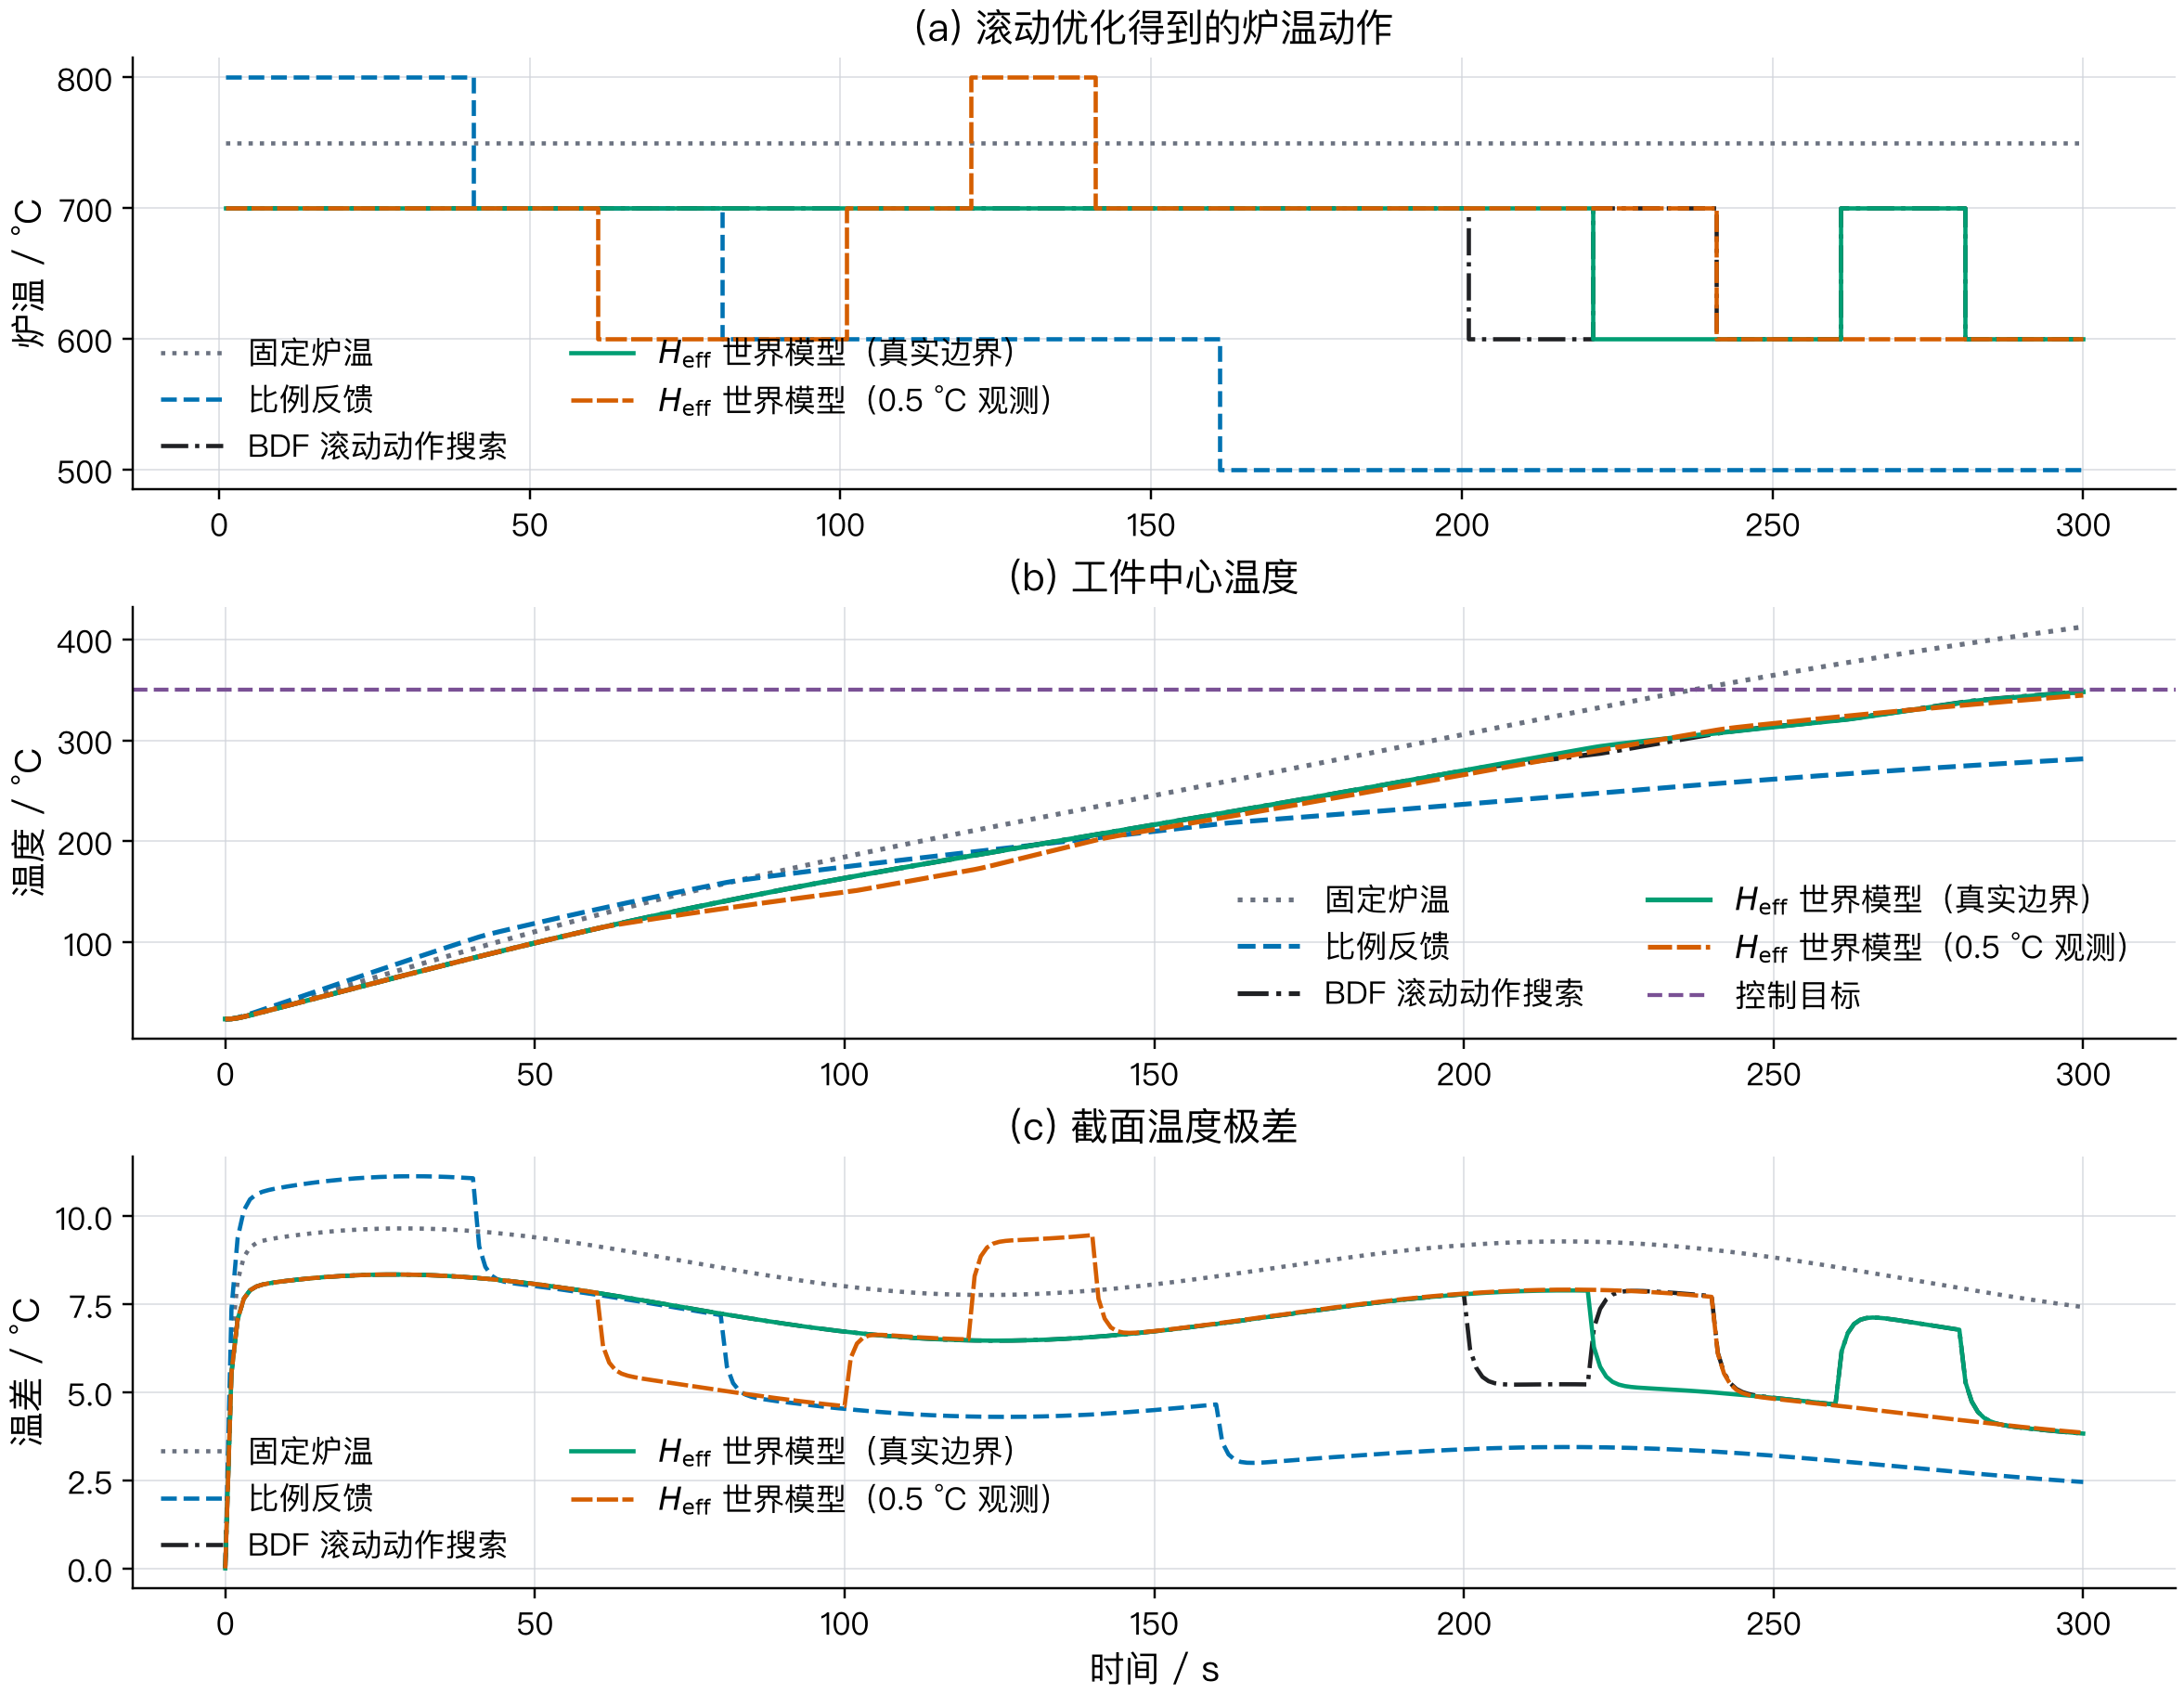
\includegraphics[width=0.96\textwidth]{closed_loop_trajectory_zh.png}
  \caption{动态边界 BDF 环境中的代表性滚动控制轨迹}
  \label{fig:closed_loop_trajectory}
\end{figure}

在相同的 10 条 ID 场景中引入五点测温，并比较四种信息条件，三个模型共形成 120 个 BDF 回合。后验均值控制的终点误差为 \SI{1.284}{\degreeCelsius}，综合目标为 16.227；风险分位控制的对应值为 \SI{1.244}{\degreeCelsius} 和 16.124。两者均为30/30个成功回合、10/10个场景全成功，95\% Wilson 区间均为 $[72.2\%,100\%]$。在这一较宽松的表面温度限制下，两种方法多次选择相同动作，尚未显示风险分位排序的明显收益。

图\ref{fig:sparse_trajectory}取模型种子 42 和联合边界轨迹 19，展示五点测量、集合状态估计和动作选择共同作用的过程。中心温度接近目标的同时，滤波器持续更新全场状态；其中的中心热电偶也持续提供对控制目标的直接测量。

\begin{figure}[H]
  \centering
  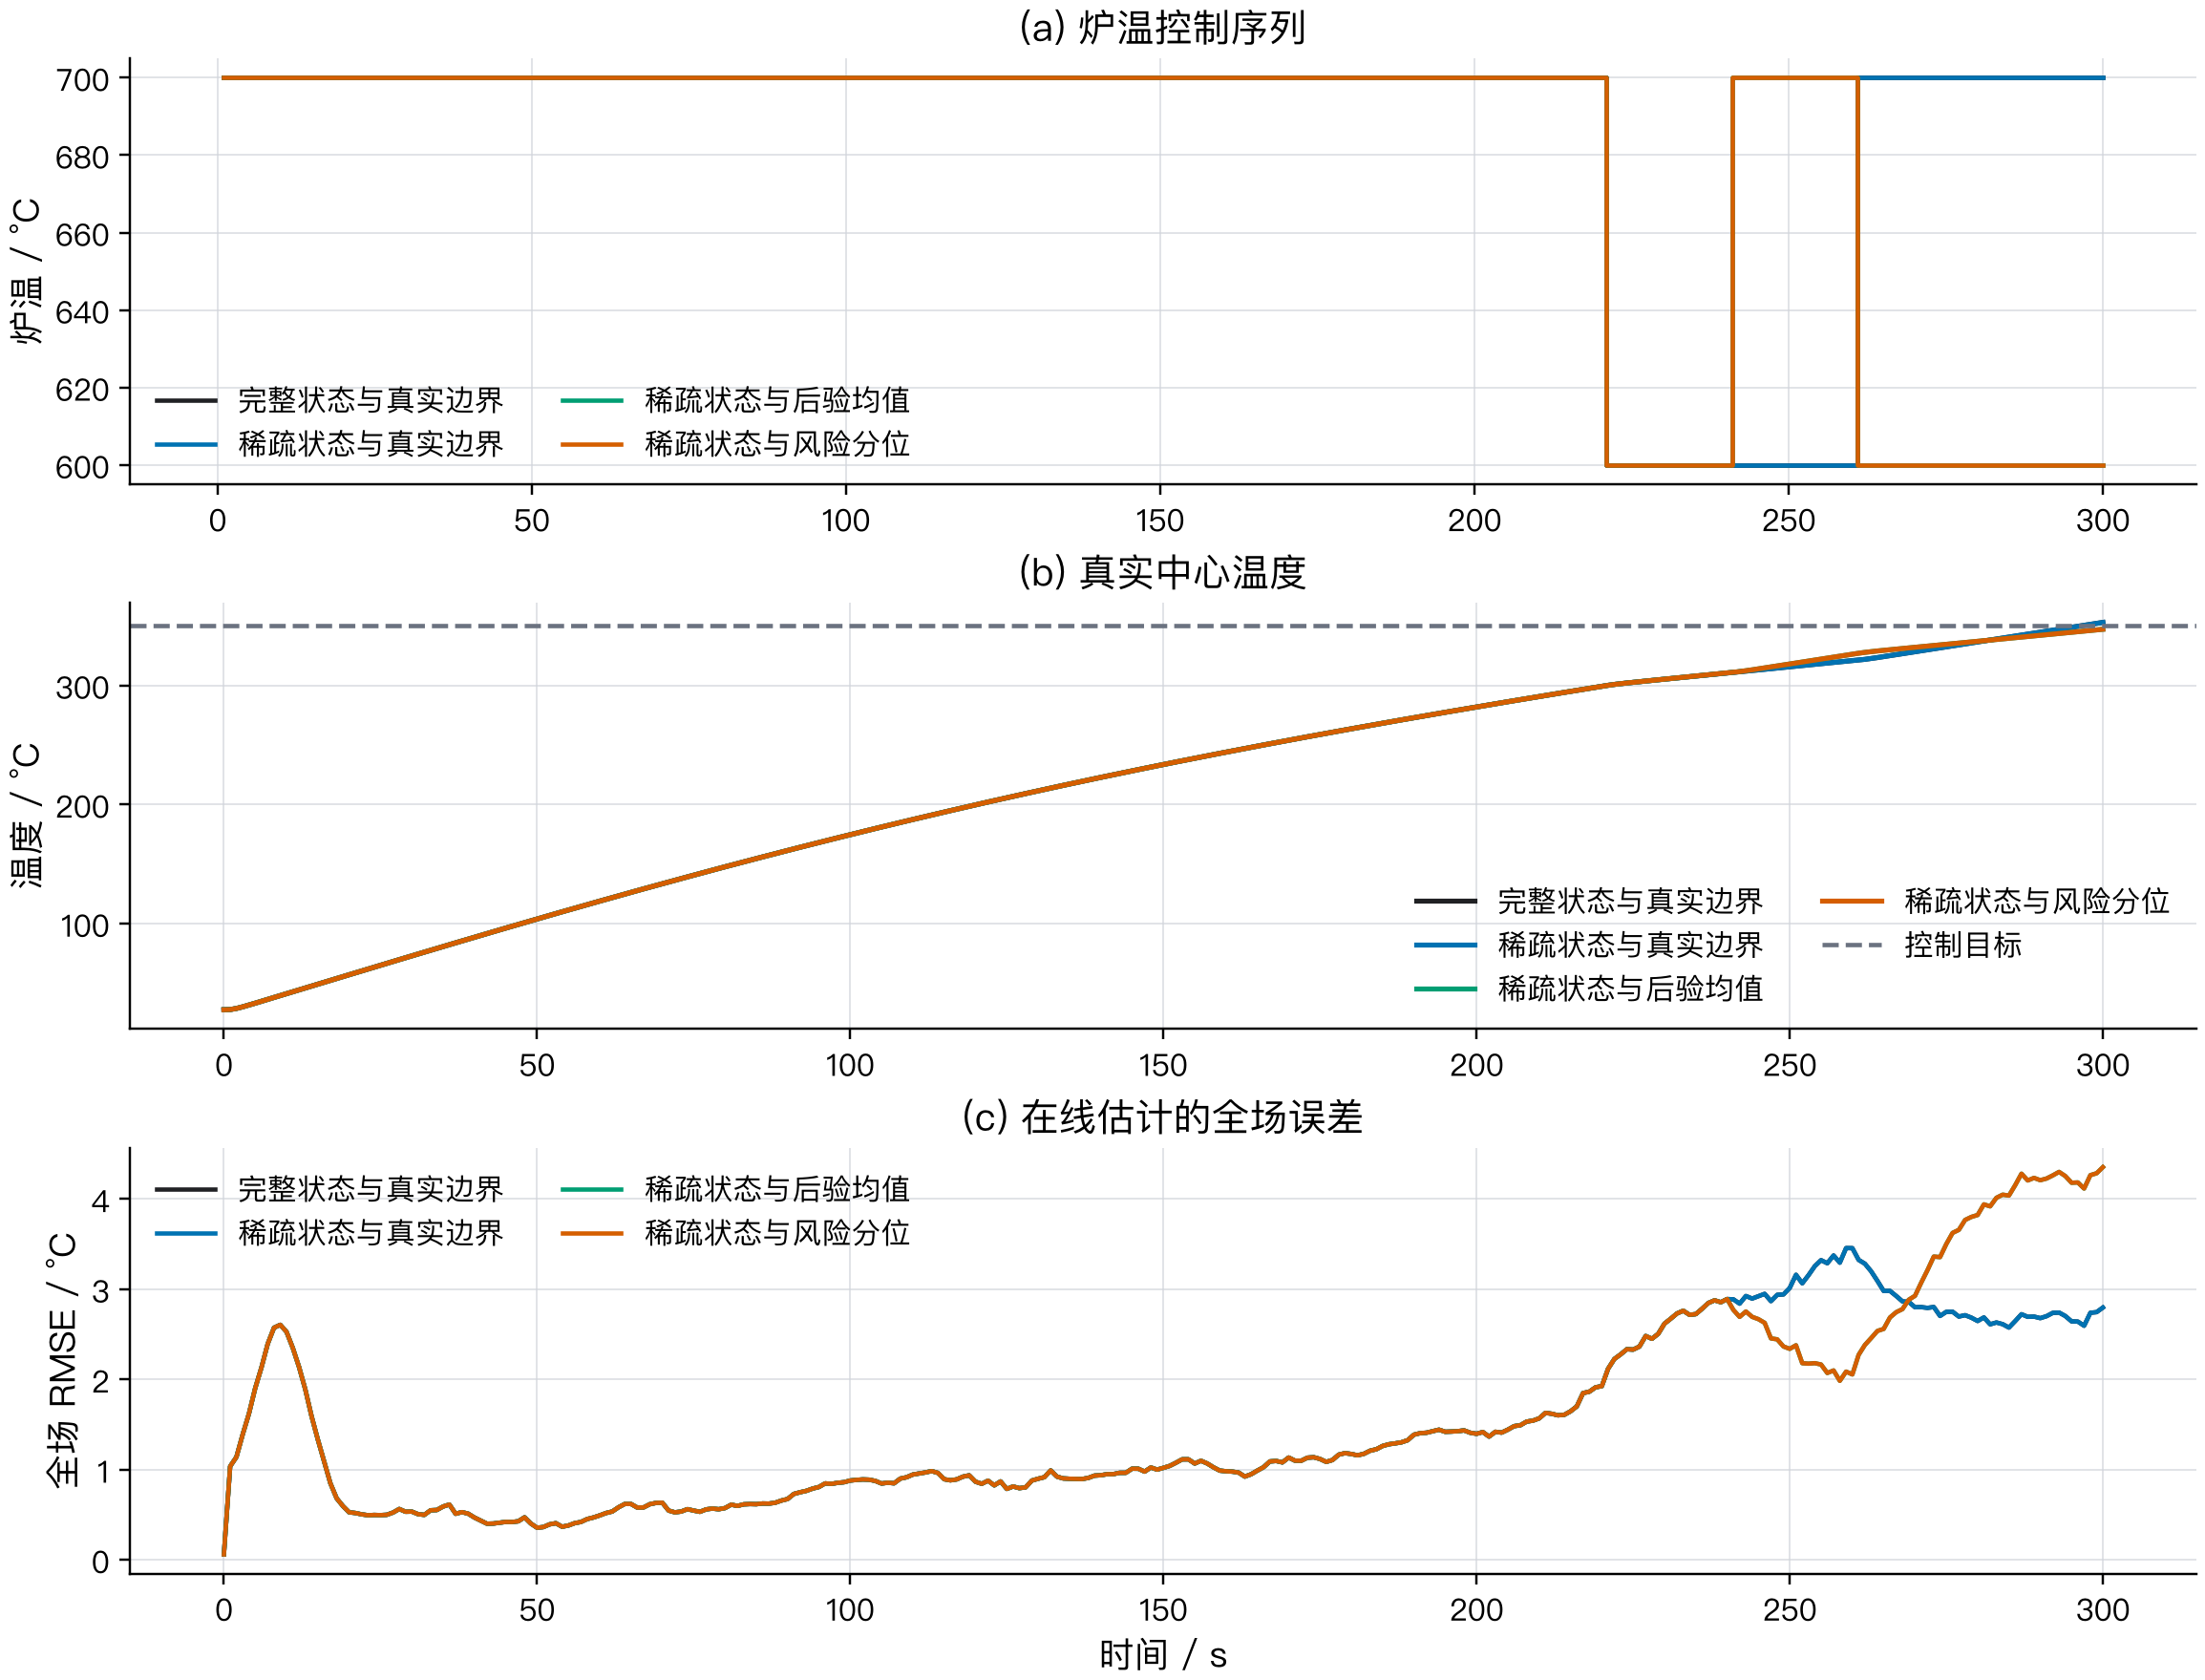
\includegraphics[width=0.96\textwidth]{sparse_observation_trajectory_zh.png}
  \caption{五点测温条件下的代表性闭环状态估计轨迹}
  \label{fig:sparse_trajectory}
\end{figure}

\subsection{删除中心测点后的配对结果}

中心测量的作用通过10条ID场景和40条独立确认参数OOD场景上的四点、五点配对实验评价，模型、滤波与控制参数保持固定。每个时刻生成五测点噪声，四点布局删除中心测量列；共同测点噪声以及滤波初始、过程噪声均相同。两种控制器、两种布局和三个模型共运行600个回合。五点分支的300个回合与对应基准的动作序列和全部非计时控制指标一致，布局比较见表\ref{tab:four_sensor_control_audit}。

\begin{table}[H]
  \centering
  \caption{四点与五点布局的闭环比较，温度指标单位：\si{\degreeCelsius}}
  \label{tab:four_sensor_control_audit}
  \small
  \resizebox{\textwidth}{!}{%
  \begin{tabular}{lcrrrcc}
    \toprule
    场景与控制器 & 测点 & 中心误差 & 平均超温 & 综合目标 & 回合成功 & 场景全成功 \\
    \midrule
    ID，后验均值 & 5 & 1.284 & 0.000 & 16.227 & 30/30 & 10/10 \\
    ID，后验均值 & 4 & 7.445 & 0.000 & 22.778 & 22/30 & 7/10 \\
    ID，风险分位 & 5 & 1.244 & 0.000 & 16.124 & 30/30 & 10/10 \\
    ID，风险分位 & 4 & 8.331 & 0.000 & 23.605 & 21/30 & 4/10 \\
    参数 OOD，后验均值 & 5 & 6.616 & 0.641 & 26.019 & 75/120 & 20/40 \\
    参数 OOD，后验均值 & 4 & 7.335 & 1.346 & 31.516 & 57/120 & 11/40 \\
    参数 OOD，风险分位 & 5 & 7.162 & 0.585 & 25.531 & 72/120 & 19/40 \\
    参数 OOD，风险分位 & 4 & 7.715 & 1.061 & 29.769 & 64/120 & 16/40 \\
    \bottomrule
  \end{tabular}}
\end{table}

在 ID 场景中，删除中心测点使后验均值控制的中心误差增加 \SI{6.161}{\degreeCelsius}，95\%配对区间为 $[4.355,8.087]$~\si{\degreeCelsius}；综合目标增加6.551，区间为 $[4.846,8.777]$。两种四点控制均未超温，主要退化表现为心部到温偏差。风险分位控制也未恢复五点条件下的跟踪精度，其场景全成功为4/10，低于后验均值控制的7/10。

在参数 OOD 确认场景中，四点后验均值控制相对五点的综合目标增加5.497，95\%区间为 $[1.483,10.368]$；回合成功比例的场景配对差为 $-15.0$ 个百分点，区间为 $[-25.8,-4.2]$ 个百分点。两种控制器的平均超温均增加，但后验均值与风险分位控制的超温配对区间分别为 $[-0.038,1.646]$ 和 $[-0.029,1.032]$~\si{\degreeCelsius}，均跨越零，不能由均值上升推定超温在总体上稳定恶化。图\ref{fig:sparse_control_audit}汇总了各工况下跟踪、超温、综合目标与成功比例的配对差。

\begin{figure}[H]
  \centering
  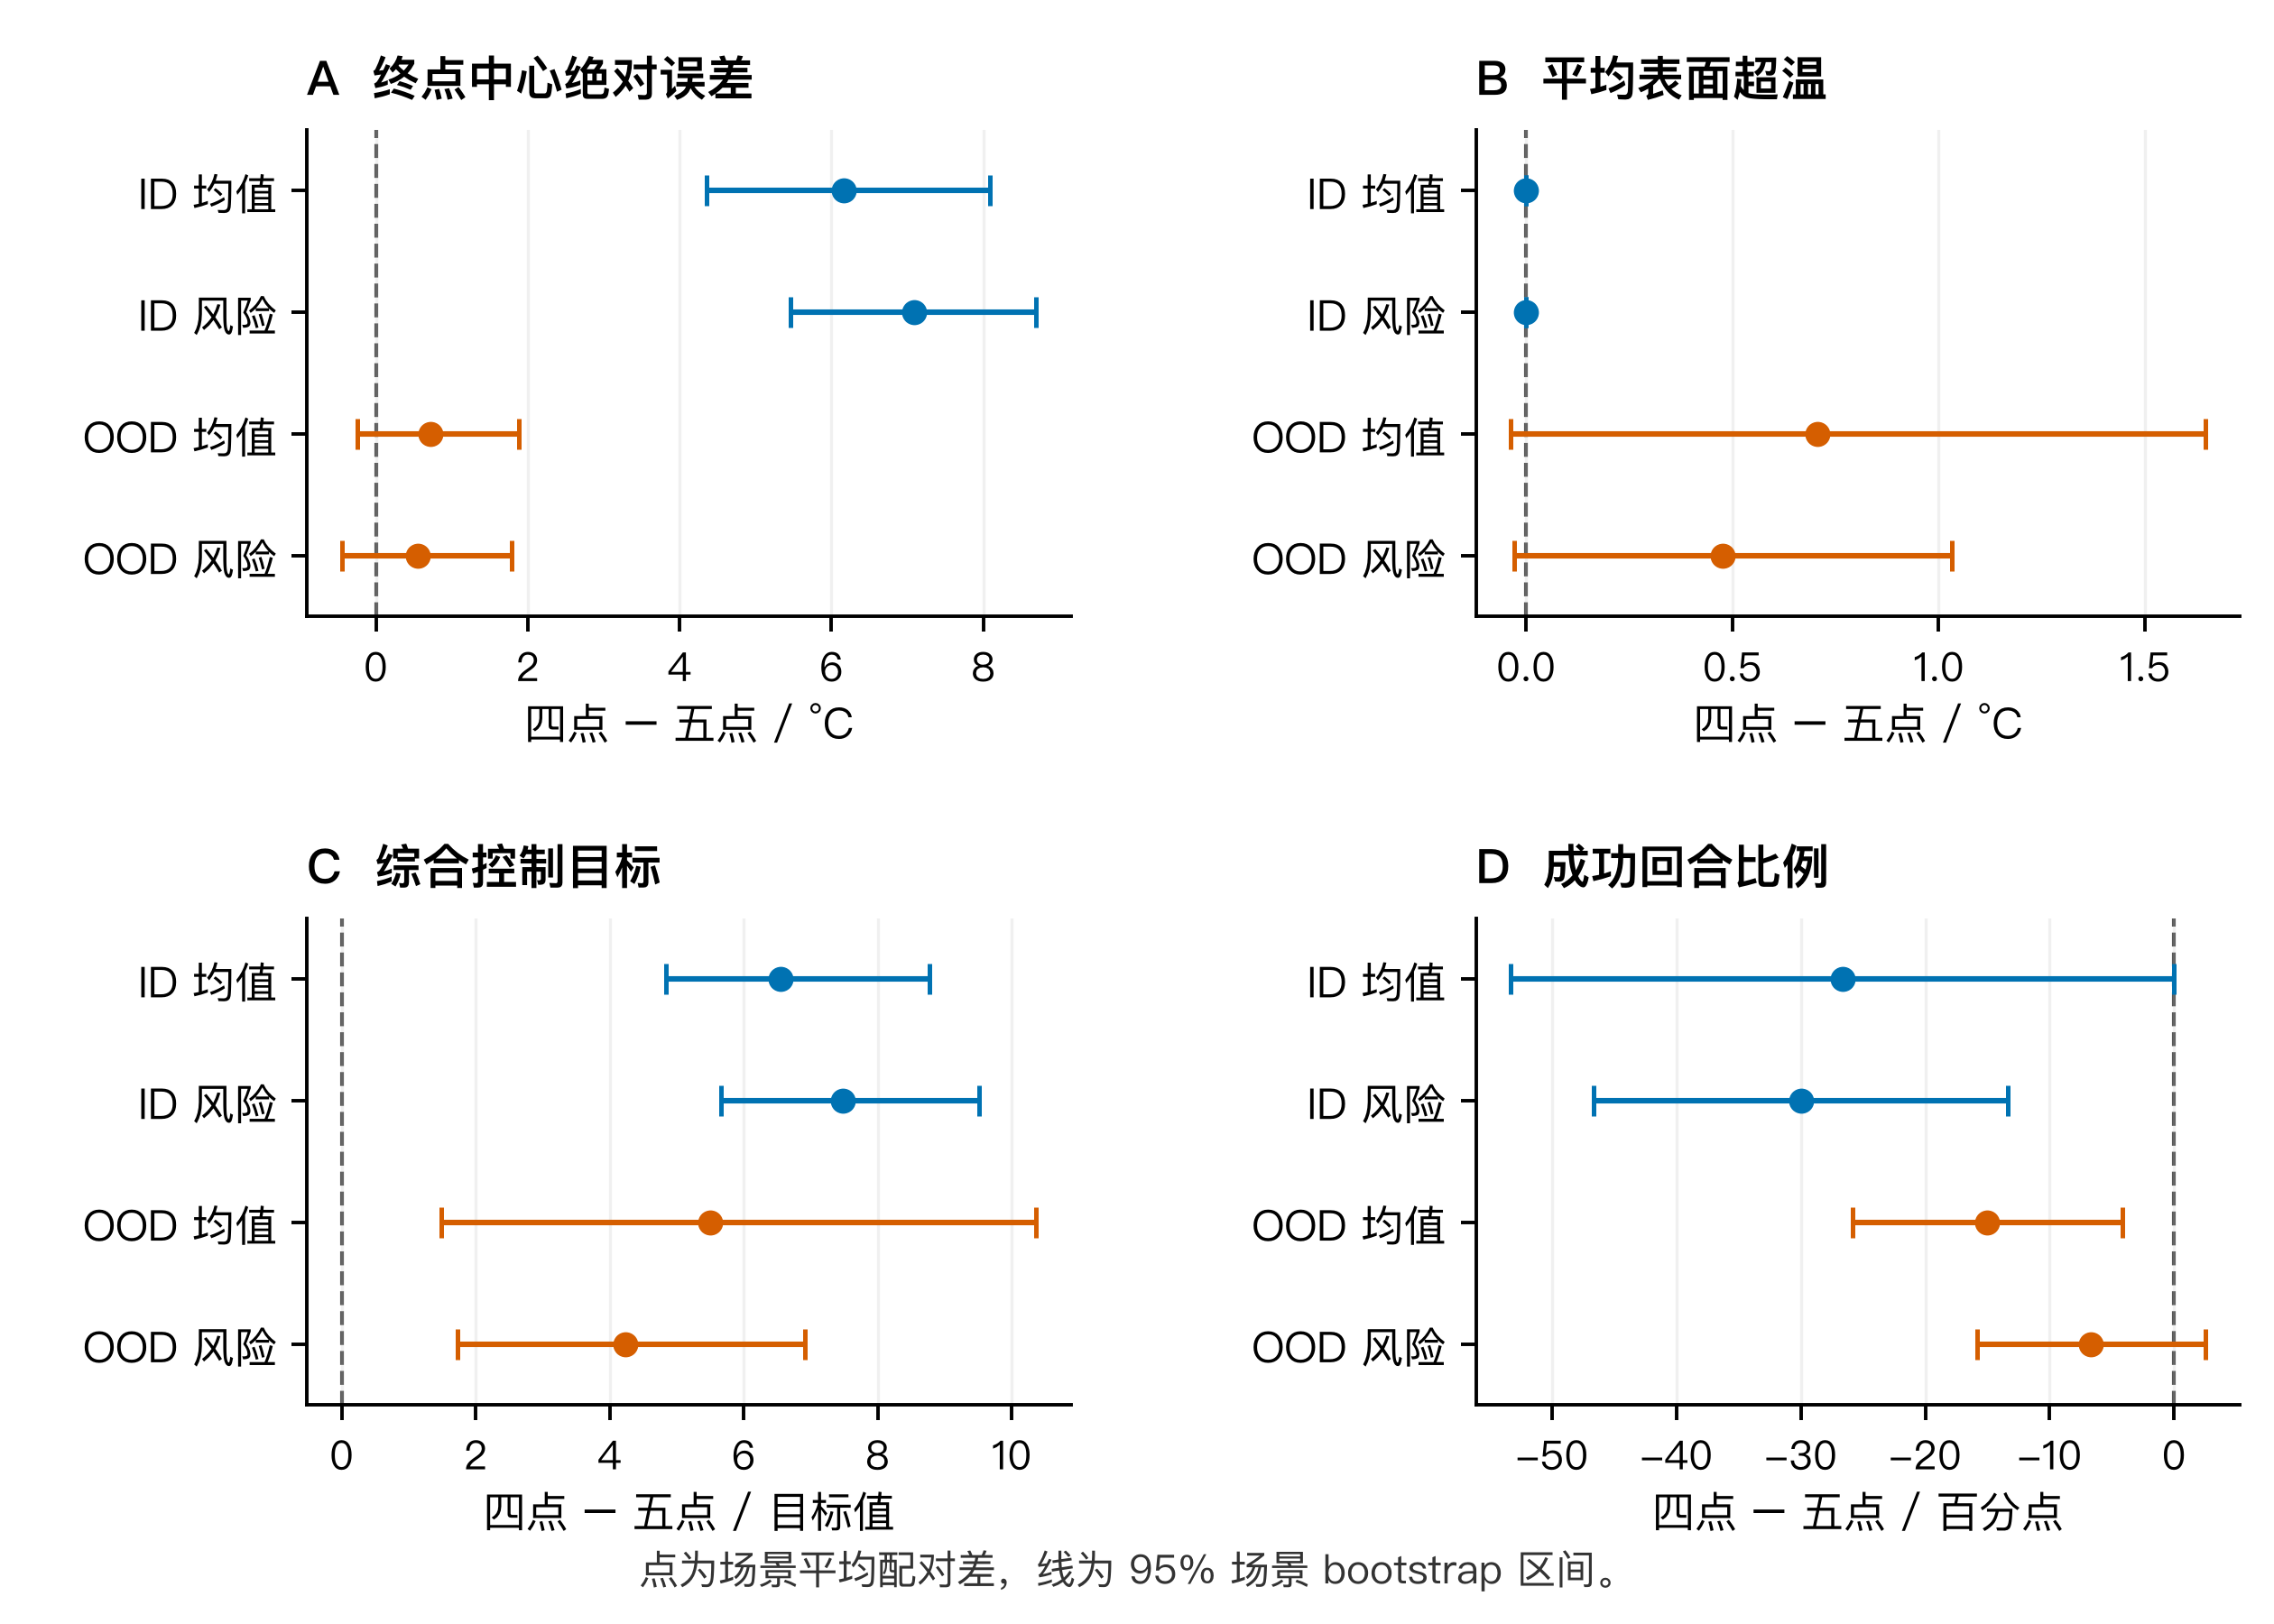
\includegraphics[width=0.98\textwidth]{sparse_control_audit.png}
  \caption{删除中心热电偶后的闭环性能变化；布局比较使用相同场景与共同随机噪声}
  \label{fig:sparse_control_audit}
\end{figure}

两种布局的闭环重建误差均在共同未观测的36个节点上计算。后验均值控制的四点、五点 RMSE 在 ID 下分别为 \SI{5.180}{\degreeCelsius}、\SI{2.216}{\degreeCelsius}，在 OOD 下分别为 \SI{7.513}{\degreeCelsius}、\SI{4.530}{\degreeCelsius}；名义90\%区间覆盖率在 ID 下为31.9\%、59.6\%，在 OOD 下为31.0\%、45.9\%。两种布局均明显欠覆盖，五点较高的控制成功比例不能作为后验区间可靠性的依据。

四点开环未测节点 RMSE 为 \SI{2.128}{\degreeCelsius} 的结果，不能直接推定相同的闭环跟踪能力或区间质量。当前方法的高 ID 成功率依赖含中心热电偶的合成观测条件；删除中心测点的退化限于本研究固定的模型、滤波和控制配置，不构成所有无中心测点方法均不可行的结论。该闭环实验使用无响应迟滞的测量，传感器响应补偿的效果仅在开环估计中得到评价。

\section{参数 OOD 下风险分位控制的证据}

风险分位控制在固定五点布局下评价，比较后验不确定性参与动作排序后的控制结果。参数 OOD 测试采用扩展边界先验，并将表面温度上限收紧为 \SI{360}{\degreeCelsius}。10条场景用于探索，互不重叠的40条场景用于独立确认探索结果；两阶段均保持后验均值与风险分位控制的配置不变。

探索集上四种控制器的结果见表\ref{tab:ood_control}。真实边界两行仍获得未来参数序列，后验两行则只使用当前估计。

\begin{table}[H]
  \centering
  \caption{10 条参数 OOD 探索场景的闭环结果，每种控制器 30 个回合}
  \label{tab:ood_control}
  \begin{tabular}{lcccc}
    \toprule
    控制器 & 中心误差/\si{\degreeCelsius} & 平均超温/\si{\degreeCelsius} & 综合目标 & 成功率 \\
    \midrule
    完整状态与真实边界 & 5.228 & 0.522 & 19.731 & $80\%$ \\
    稀疏状态与真实边界 & 5.119 & 0.750 & 20.665 & $80\%$ \\
    稀疏状态与后验均值 & 5.966 & 0.302 & 21.376 & $70\%$ \\
    稀疏状态与风险分位 & 5.822 & 0.181 & 19.638 & $70\%$ \\
    \bottomrule
  \end{tabular}
\end{table}

表中的80\%和70\%分别为24/30和21/30个成功回合，仅是执行记录比例。按场景全成功判据，四行依次为7/10、8/10、7/10、7/10；7/10与8/10的95\% Wilson区间分别为 $[39.7\%,89.2\%]$ 和 $[49.0\%,94.3\%]$。风险分位相对后验均值控制的场景配对差见表\ref{tab:risk_paired}。

\begin{table}[H]
  \centering
  \caption{10 条探索场景中风险分位减后验均值的配对统计}
  \label{tab:risk_paired}
  \begin{tabular}{lcccc}
    \toprule
    指标 & 后验均值控制 & 风险分位控制 & 平均配对差 & 95\% bootstrap 区间 \\
    \midrule
    综合目标 & 21.376 & 19.638 & $-1.737$ & $[-3.291,-0.226]$ \\
    平均超温/\si{\degreeCelsius} & 0.302 & 0.181 & $-0.121$ & $[-0.363,0.000]$ \\
    中心误差/\si{\degreeCelsius} & 5.966 & 5.822 & $-0.143$ & $[-0.720,0.454]$ \\
    \bottomrule
  \end{tabular}
\end{table}

综合目标在10个场景中有7个改善、1个不变、2个增加，平均配对差的区间低于零。平均超温降低40.0\%，但差异集中于一个高表面热负荷场景，其余9个场景均未超温；中心误差区间跨越零。每回合规划时间由 \SI{0.098}{\second} 增至 \SI{0.240}{\second}。探索集的综合目标下降伴随规划时间增加，且超温收益集中于少数场景；有限样本尚不足以支持风险分位控制的稳定优势。

\begin{figure}[H]
  \centering
  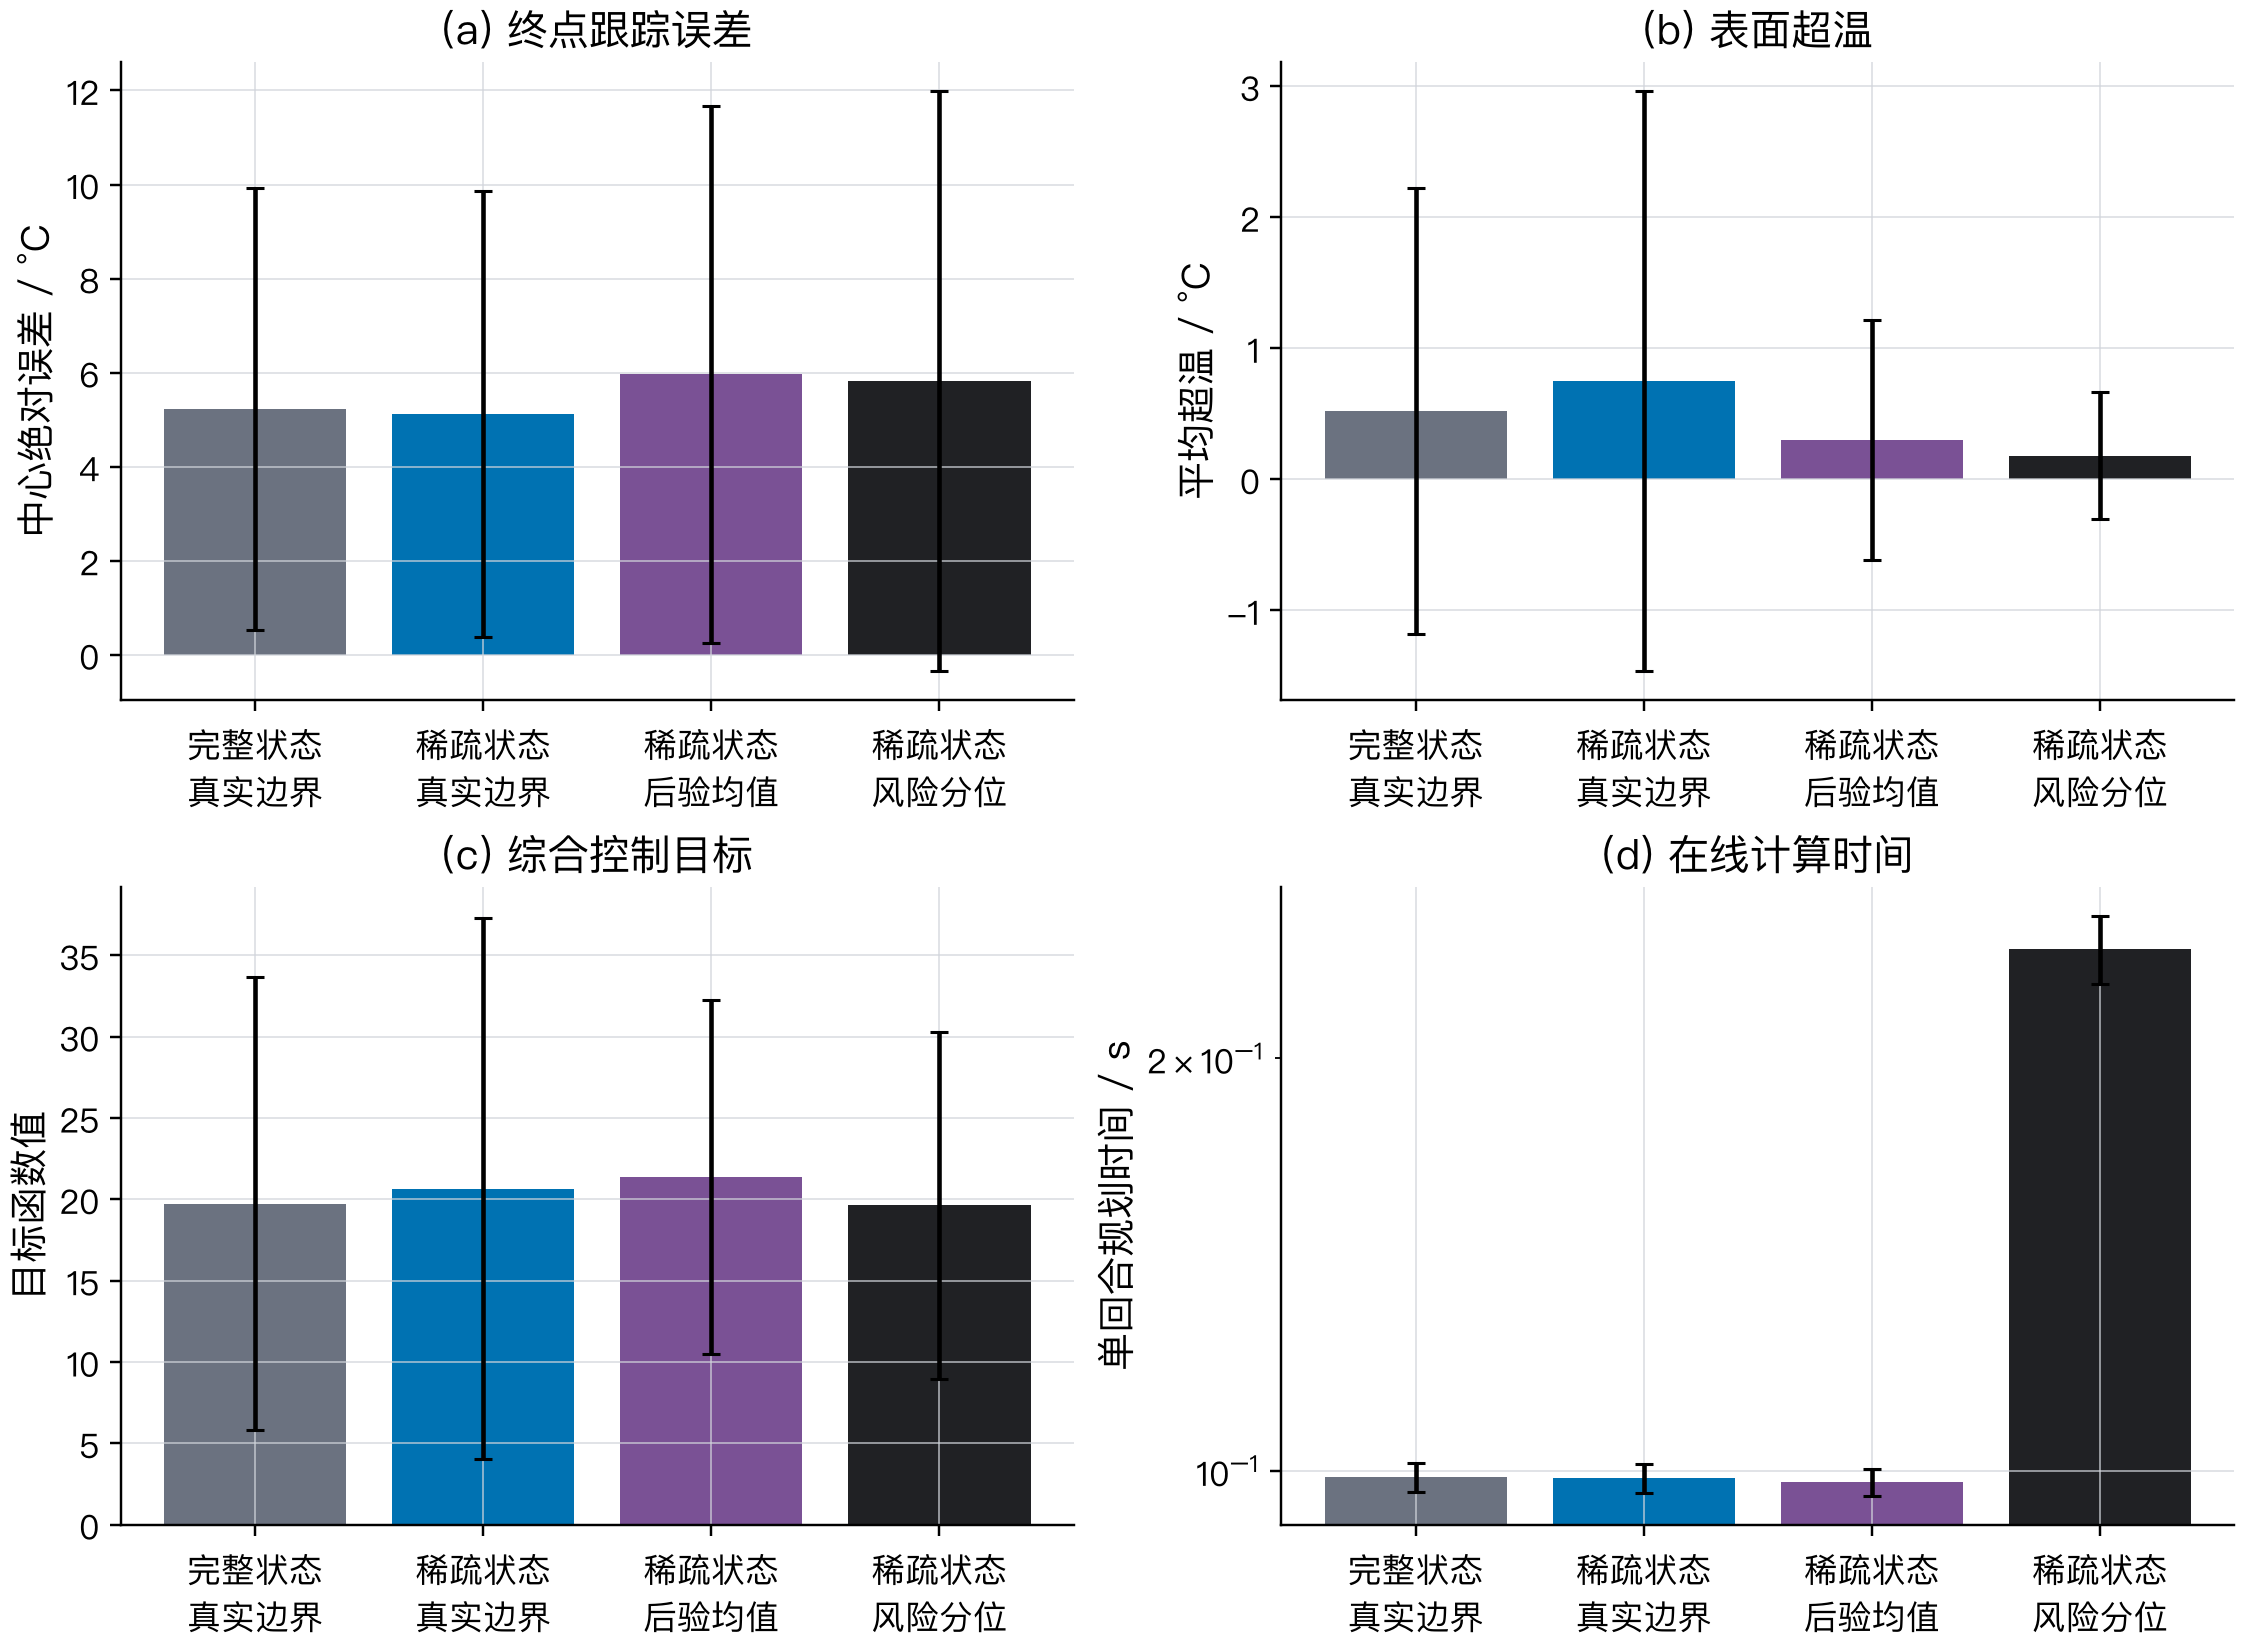
\includegraphics[width=0.96\textwidth]{ood_closed_loop_control.png}
  \caption{10 条探索场景在收紧表面温度约束后的闭环结果}
  \label{fig:ood_control}
\end{figure}

确认集从同一参数 OOD 数据池中另取40条场景，每个类别8条，排除全部探索场景。两种后验控制器各执行120个回合，以相同的场景配对口径计算结果，见表\ref{tab:risk_confirmatory}。确认集与探索集的独立性限于场景不重叠，三个训练模型仍为同一固定面板。

\begin{table}[H]
  \centering
  \caption{40 条独立确认场景中风险分位减后验均值的配对统计}
  \label{tab:risk_confirmatory}
  \resizebox{\textwidth}{!}{%
  \begin{tabular}{lcccc}
    \toprule
    指标 & 后验均值控制 & 风险分位控制 & 平均配对差 & 95\% bootstrap 区间 \\
    \midrule
    综合目标 & 26.019 & 25.531 & $-0.488$ & $[-2.802,1.950]$ \\
    平均超温/\si{\degreeCelsius} & 0.641 & 0.585 & $-0.056$ & $[-0.527,0.418]$ \\
    中心误差/\si{\degreeCelsius} & 6.616 & 7.162 & 0.546 & $[0.070,1.029]$ \\
    成功率 & $62.5\%$ & $60.0\%$ & $-2.5$ 个百分点 & $[-8.3,2.5]$ 个百分点 \\
    \bottomrule
  \end{tabular}}
\end{table}

确认集中，后验均值与风险分位控制的场景全成功数分别为20/40、19/40，95\% Wilson区间分别为 $[35.2\%,64.8\%]$、$[32.9\%,62.5\%]$；场景全成功数与表中的回合成功比例62.5\%、60.0\%对应不同统计对象。综合目标有23个场景改善、1个不变、16个增加。平均差仍偏向风险分位控制，但综合目标、超温和成功比例的95\%配对区间均跨越零；中心误差平均增加 \SI{0.546}{\degreeCelsius}，区间为 $[0.070,1.029]$~\si{\degreeCelsius}。确认结果未支持风险分位控制稳定降低综合目标或提高成功比例，并显示出中心跟踪误差增加。图\ref{fig:ood_control_extension}展示了确认集的配对差分布。

\begin{figure}[H]
  \centering
  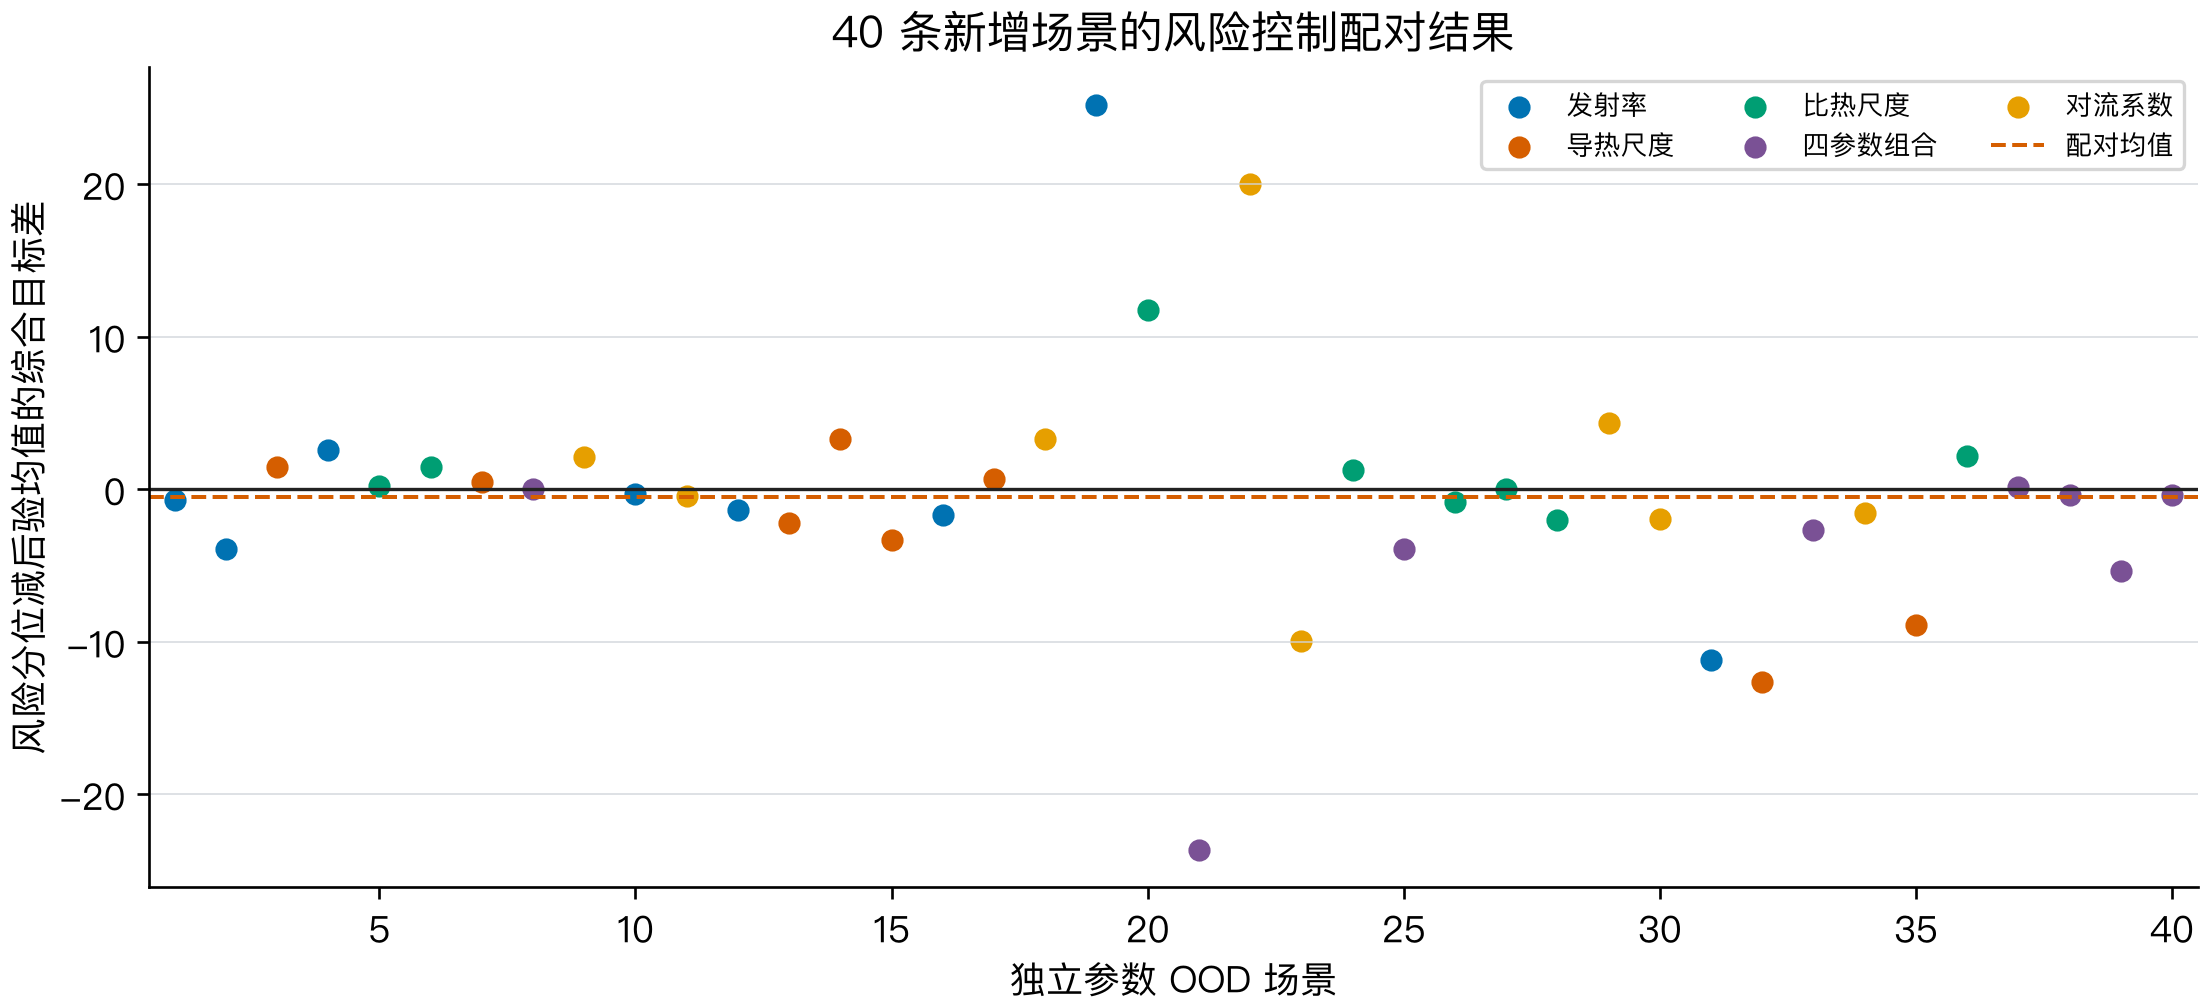
\includegraphics[width=0.94\textwidth]{ood_control_extension.png}
  \caption{40 条独立确认场景的风险控制综合目标配对差}
  \label{fig:ood_control_extension}
\end{figure}

合并两组场景作事后描述，50 条场景的综合目标配对差为 $-0.738$，95\%区间为 $[-2.630,1.248]$，仍跨越零。该合并不能替代独立确认结果，也不构成预先统一设计的50场景检验。

在本研究的数值环境和固定配置下，中心测量直接影响闭环跟踪精度，反馈轨迹上的后验区间存在欠覆盖。风险分位控制未在确认场景中表现出稳定的综合收益，四点布局下仍未达到五点布局的跟踪精度。世界模型与集合滤波构成的滚动控制器，其控制误差、成功比例及区间覆盖率均受观测条件限制。

\chapter{结论与展望}

\section{主要结论}

本文建立了结合神经递归预测、状态估计与炉温决策的热过程模型。模型以完整离散温度场为状态，显式接收炉温动作，并在包含温变物性和对流辐射边界的 C45/AISI 1045 类中碳钢数值环境中验证。实验评价了完整轨迹预测、动态边界表示及有限测温下的闭环性能。

\subsection{递归预测精度与计算效率}

物理约束的收益主要体现在离散方程一致性和部分参数外推任务。一维控制曲线 OOD 的离散残差降低 $44.8\%$，逐轨迹温度 RMSE 的配对区间未支持稳定改善；四参数组合 OOD 的滚动 RMSE 降低 $29.5\%$，最大误差由 \SI{121.76}{\degreeCelsius} 降至 \SI{61.69}{\degreeCelsius}。在固定三维几何中，基础与加密网格的三种子 OOD 离散残差分别降低 $12.5\%$ 和 $25.6\%$，两网格的温度精度配对区间均跨零。物理残差与温度误差的改善程度存在差异：前者反映对训练所用离散方程的一致性，后者仍需独立评价。现有结果未支持普遍的 OOD 温度精度优势。

在相同 100 条物理场景的完整推演计时中，81 节点 BDF 的中位耗时为自主有效边界网络的 $44.0$ 倍，41 节点固定步长数值模型为该网络的 $1.06$ 倍，且数值模型误差更低。网络相对 BDF 的耗时优势与固定步长模型的近似耗时并存，一维单轨迹结果尚未建立网络相对于合适数值算法的精度与效率综合优势。

\subsection{等效边界表示及其可辨识条件}

在本文一维对称、单一表面温度且 $h(t),\varepsilon(t)$ 逐时自由变化的瞬时观测模型下，当前热流约束的是 $\Heff=h+\varepsilon h_{\mathrm{rad}}$。两组模型在推演时获得相同初态、炉温及真实动态 $h,\varepsilon$，有效边界模型由自身预测表面温度逐步重算 $\Heff$。该表示使滚动 RMSE 从 $2.285\pm0.108$ 降至 $1.494\pm0.082$~\si{\degreeCelsius}；BDF 参考下从 $2.316\pm0.092$ 降至 $1.560\pm0.092$~\si{\degreeCelsius}。两组轨迹配对区间均支持改善。训练与验证选模使用参考状态构造 $\Heff$，测试阶段使用已知动态边界，因此该比较的结论限定于边界已知时的预测表示，未覆盖未知边界下的全流程辨识。

炉温变化会改变辐射等效系数。本文构造的五组参数在当前动作下等效，测试候选炉温改变后，组间最大热流差为 \SI{12.03}{\kilo\watt\per\square\metre}。控制模型据此保留受历史数据和先验约束的 $h,\varepsilon$ 后验，并按候选动作计算对应的边界输入。当前估计的单一 $\Heff$ 无法唯一确定这些候选动作下的热流，对任意有限时间状态转移的充分性也未得到证明。该结论针对逐时自由变化参数的局部瞬时观测；参数恒定、激励充分或存在多个独立表面温度约束时，辨识条件需另行分析。

\subsection{观测条件与闭环控制性能}

稀疏测温可以在本文先验与数值条件下支持内部温度估计。无中心测点的四点方案取得 \SI{2.128}{\degreeCelsius} 的开环未测节点 RMSE；加入 \SI{5}{\second} 响应滞后后，误差增至 \SI{4.894}{\degreeCelsius}。用独立校准轨迹标定响应并增广传感器状态后，误差降至 \SI{2.178}{\degreeCelsius}，90 条轨迹的配对区间支持改善。名义 $90\%$ 区间覆盖率由 $34.4\%$ 升至 $84.2\%$，仍存在覆盖不足。该证据适用于合成一阶传感器的开环估计，尚未覆盖带滞后的闭环控制。

中心测点对当前配置下的闭环控制具有明显影响。ID 后验均值控制中，含中心测点的五点方案完成 $30/30$ 个成功回合，对应 $10/10$ 个场景的三个固定模型均成功；删去中心测点后，中心误差由 \SI{1.284}{\degreeCelsius} 增至 \SI{7.445}{\degreeCelsius}，成功回合为 $22/30$，场景全成功为 $7/10$。严格参数 OOD 下，四点相对五点的综合目标增加 $5.497$，95\% 配对区间为 $[1.483,10.368]$。四点方案的开环估计精度未转化为与五点方案相近的控制性能。该比较采用冻结的滤波和控制配置，对其他无中心测点方案的可行性不作推断。

风险分位控制的效果具有场景依赖性。40 条独立参数 OOD 场景中，五点风险分位控制相对后验均值控制的目标差为 $-0.488$，95\% 配对区间为 $[-2.802,1.950]$，未确认探索性样本中的综合收益。参数集合提供了候选动作的不确定性描述；闭环温度后验的明显欠覆盖限制了这一描述的概率解释，当前控制器尚不具备经校准的概率安全保证。

\section{方法的应用位置与适用范围}

本文系统适合作为上层热状态估计与候选工艺评价的方法原型。少量热电偶提供观测，集合滤波更新内部温度与边界后验，递归模型据此推演候选炉温，滚动搜索向下层控制回路提供设定值。这一结构与工业加热炉的模型化规划和预测控制具有共同的功能分工\cite{steinboeck2011trajectory,steinboeck2013nmpc,yi2017tracking}。当前实验支持在明确物理模型、观测条件和参数范围下研究该链路，尚不能据此量化实际生产中的节能、质量改善或工艺周期收益。

研究范围由数值环境与信息假设共同限定。一维实验采用对称平板，三维实验采用固定长方体与均匀六面边界；材料函数和几何已知，闭环从已知均匀初温开始。BDF 交叉验证改变了网格和时间积分方法，共享连续传热方程与材料函数，评价范围限于相同传热假设下的数值实现变化，尚缺乏真实炉体的独立验证。三维两套网格分别训练或迁移训练模型，尚未证明共享模型的跨网格收敛或跨几何泛化，也未形成三维稀疏测温闭环结果。

模型描述热动力学子问题，不含显式相变组织演化、热应力和变形状态。控制任务在 \SI{300}{\second} 内跟踪 \SI{350}{\degreeCelsius} 目标，仅用于方法测试，不构成完整工业热处理制度。现有实验未接入真实炉温、热电偶或执行器数据，传感器响应补偿与后验风险评价均需在实际测量中重新检验。

\section{后续研究方向}

真实炉体验证需要独立的校准与评价数据。仪器化试块的表面和内部测温可用于确定物性、边界先验与传感器响应，独立炉次用于评价完整轨迹误差及预测区间覆盖率。传感器模型应包含时间常数漂移和非一阶响应，控制评价应纳入执行器速率、饱和及真实炉温跟踪误差。这些因素影响数值环境中的估计和控制结果向实际工况迁移时的误差。

方法比较应以任务要求的精度为共同约束。在固定几何与更复杂几何上，可比较优化数值积分、降阶模型和物理信息算子\cite{wang2021pideeponet,derouiche2021induction,gong2026heatrom}，联合报告离线成本、在线候选数量、延迟与误差。相对参考求解器的加速比需结合参考精度和算法配置解释。对控制中不确定性较大的候选，可引入数值求解器复核，并评价复核开销对决策时限的影响。

测点位置、传感器动态、滤波参数与控制目标可纳入联合设计。中心测点删除实验所显示的性能变化，为比较不同观测配置提供了依据；后续评价可采用独立场景，在相近控制质量下比较测量成本。风险控制的概率可靠性需通过部署分布下的后验校准、区间覆盖率及约束违例频率共同检验。


\begingroup
\small
\setstretch{1.12}
\printbibliography[heading=bibintoc,title={参考文献}]
\endgroup

\appendix

\chapter{复现信息}
\section{代码、模型与版本对应}

论文代码仓库与模型权重托管地址分别为
\begin{center}
  \url{https://github.com/khakhasshi/heat-treatment-world-model}\\
  \url{https://huggingface.co/JIANGJINGZHE/heat-treatment-world-model}
\end{center}
代码包含控制体守恒离散求解器、神经动力学训练与评价、边界观测器、集合滤波器、滚动控制及绘图程序。公开版本以 \path{thesis-open-release-v1} 标识，其权重映射和 SHA-256 值见 \path{docs/huggingface-weights-manifest.csv}。公开权重清单记录已发布模型，本地快照清单记录本文实验的完整输入，两者分别核对。

本文对应本地快照 \path{thesis-scientific-style-20261010}，包含未提交修改，尚未公开发布。本次文字修订与校验记录见
\begin{center}
  \path{docs/thesis-scientific-style-20261010.md}
\end{center}
源文件、正式结果、模型输入和两版导出 PDF 的内容校验值记录在
\begin{center}
  \path{docs/thesis-scientific-style-20261010-manifest.json}
\end{center}
该快照沿用已完成的数值实验及其训练配置。正文组织与实验取数关系见
\begin{center}
  \path{docs/thesis-integrated-revision-20261010.md}
\end{center}
下列历史实验版本的记录独立保留：
\begin{center}
  \small\texttt{experiment-freeze-v1}\\
  \texttt{thesis-revision-v2-20260905}\\
  \texttt{thesis-audit-followup-20261001}
\end{center}

\section{实验组织与复现入口}

实验按独立物理轨迹划分训练、验证与测试集；模型检查点依据完整验证轨迹误差选择。各专题的采样范围、随机种子、网格、超参数与正式指标见 \path{docs/experiment-freeze.md} 及其链接。预测、估计与控制实验具有各自的信息条件，使用真实边界的预测对照仅评价边界已知时的预测性能，未知边界的在线估计采用独立实验评价。

第四章的一维训练与 OOD 实验使用以下命令行入口，依次对应模型比较、参数范围外推和边界时间结构外推：
\begin{center}
  \small\texttt{compare-heat-world-models}\\
  \texttt{evaluate-parameter-ood}\\
  \texttt{evaluate-dynamic-boundary-ood}
\end{center}
第五章的状态估计、传感器扰动和控制实验入口如下。响应状态补偿使用独立校准轨迹，参数 OOD 的探索与确认场景分别保存。
\begin{center}
  \small\texttt{evaluate-partial-observability}\\
  \texttt{evaluate-sensor-robustness}\\
  \texttt{evaluate-closed-loop-control}\\
  \texttt{evaluate-ood-partial-observability}\\
  \texttt{analyze-ood-control-extension}
\end{center}
模块形式的入口统一以 \path{heat_world_model} 为包名，使用下列调用方式：
\begin{center}
  \small\texttt{PYTHONPATH=src .venv/bin/python -m}\\
  \texttt{heat\_world\_model.}\textit{模块名}
\end{center}
\begin{table}[H]
  \centering
  \small
  \caption{专题评价的模块入口}
  \begin{tabular}{ll}
    \toprule
    评价内容 & 模块名 \\
    \midrule
    同信息边界与完整推演计时 & \texttt{fair\_boundary\_audit\_cli} \\
    三维动作与模型评价 & \texttt{three\_dimensional\_action\_audit\_cli} \\
    传感器响应状态补偿 & \texttt{sensor\_response\_cli} \\
    四点与五点闭环对照 & \texttt{sparse\_control\_audit\_cli} \\
    独立场景成功率 & \texttt{scenario\_success\_audit\_cli} \\
    \bottomrule
  \end{tabular}
\end{table}
边界表示对照的 \texttt{--mode evaluate} 与完整推演计时的 \texttt{--mode benchmark} 分开运行，两种参考求解器使用相同的 100 条场景。计时阶段固定硬件和线程配置，并暂停其他重计算任务。三维两网格共享 96 条工况，采用零阶保持动作，各自按对应网格参考场训练和验证。测点闭环比较共享场景和共同测点的随机扰动。

具体参数以冻结协议为准；正式结果、原始逐轨迹记录及二进制输入的对应关系见
\begin{center}
  \path{docs/thesis-audit-followup-20261001.md}\\
  \path{outputs/c45_audit_followup_20261001/}
\end{center}
完整性核对可执行
\begin{center}
  \small\texttt{python3 scripts/freeze\_thesis\_revision.py --manifest}\\
  \path{docs/thesis-scientific-style-20261010-manifest.json}
\end{center}

\section{协议溯源与结果使用边界}

有效边界模型的训练和验证选模使用参考温度构造 $\Heff$，测试时的自主表示对照只依赖预测表面温度与已知真实边界历史。参考状态条件输入的结果与自主推演指标分别记录。控制实验中的真实状态或真实未来边界输入均单独标明，相应结果仅适用于所注明的信息条件。

三维实现记录保留了动作离散方式的核查过程。早期参考轨迹从前一炉温向当前指令线性变化，网络输入只包含当前动作；正文采用与网络输入一致的零阶保持参考及匹配训练预算。两种动作定义下，基础网格 OOD 参考轨迹的差异为 RMSE \SI{1.415}{\degreeCelsius}、最大绝对差 \SI{13.148}{\degreeCelsius}，两项数值均描述参考解的变化。基础网格物理模型的训练预算由 25 轮改为与数据模型一致的 40 轮，动作定义与训练预算的共同变化限制了对版本间网络误差差异的单因素归因。剖面图固定为全局工况 74 的 \SI{192}{\second} 时刻；该工况最初按 ID 数据模型误差接近上四分位数选取，时刻按参考场内部温差最大选取。图中展示该选例在最终协议下的温度场，总体性能以完整测试集统计为准。原始记录、协议和选例信息均保留在相应结果目录。

控制实验中，10 条探索性 OOD 场景与 40 条独立确认场景分别报告。三种训练种子作用于同一场景时构成重复模型评价，独立物理样本数按场景计。论文的场景成功指标要求三个固定模型均成功；其区间只反映当前模型面板与场景样本下的不确定性。配对分析以各场景内的模型指标均值之差为统计量，以场景为重采样单位，与总体 RMSE 均值的直接相减具有不同统计含义。

\section{学术诚信与引用说明}

公开材料用于学习、研究复现和方法参考。复用代码、图表、实验结果或模型输出时，应标注来源、修改范围及所用版本或权重文件。具体说明和推荐引用信息见 \path{ACADEMIC_USE_NOTICE.md} 与 \path{CITATION.cff}。

\end{document}
